\documentclass[conference,onecolumn]{IEEEtran}
\usepackage{hyperref}
\usepackage[utf8]{inputenc}
\usepackage[french]{babel}
\usepackage{amsmath,amssymb,amsfonts}
\usepackage{mathtools}
\usepackage{algorithmic}
\usepackage{graphicx}
\usepackage{textcomp}
\usepackage{xcolor}
\usepackage{float}
\usepackage{lipsum, babel}
\usepackage[T1]{fontenc}
\usepackage{biblatex}
\usepackage{ragged2e}
\usepackage{geometry}
\usepackage{csquotes}
\geometry{
   hmargin=3cm,
   vmargin=2cm,
   includeheadfoot
}
\DeclareMathOperator{\sinc}{sinc}

\pagestyle{plain}

% Inicio del documento
\begin{document}

\title{Atténuation du bruit dans les enregistrements audio en implémentant deux méthodes classiques et une méthode hybride \\
}

\author{\IEEEauthorblockN{1\textsuperscript{st} José Miguel Galindo Barco}
\IEEEauthorblockA{\textit{Ecole d’ingénieurs}\\
\textit{Génie de systèmes} \\
\textit{Université EAFIT}\\
\href{mailto:jmgalindob@eafit.edu.co}{jmgalindob@eafit.edu.co}
}
\and
\IEEEauthorblockN{2\textsuperscript{nd} Juan José Tamayo Acevedo}
\IEEEauthorblockA{\textit{Ecole de sciences}\\
\textit{Génie mathématique} \\
\textit{Université EAFIT}\\
\href{mailto:jjtamayoa@eafit.edu.co}{jjtamayoa@eafit.edu.co}
}
\and
\IEEEauthorblockN{3\textsuperscript{rd} Salomón Cardeño Luján}
\IEEEauthorblockA{\textit{Ecole de sciences}\\
\textit{Génie mathématique} \\
\textit{Université EAFIT}\\
\href{mailto:scardenol@eafit.edu.co}{scardenol@eafit.edu.co}
}
}

\maketitle

\begin{abstract}
L’atténuation du bruit est un domaine d’étude actif dans des milieux comme le traitement digital et analogique des signaux. Dans ce domaine il existe une grande variété d’algorithmes et/ou méthodes classiques et modernes qui sont utilisé dans ce but. Dans ce travail de recherche, nous réaliserons une étude théorique du filtre analogique passe-bas avec une approximation de Butterworth, le filtre de Weiner et la méthode dite hybride de DSP/Deep Learning RNNbruit. Puis nous développerons une analyse de ces trois méthodes où nous comparerons les résultats de signaux lorsque nous filtrons un signal propre, un signal avec addition de bruit blanc, un signal avec addition de bruit rosa et un signal avec addition de bruit rouge. Les enregistrement audios résultant de chaque méthode filtrage seront comparer qualitativement et quantitativement, d’où la nécessité de tenir en compte la perception auditive du récepteur. Finalement, nous proposerons des modifications sur la mise en œuvre ou implémentation de ces méthodes en considérant le contexte et le bon fonctionnement dans ce dernier. 
\end{abstract}


\section{Introduction}
De nos jours, de plus en plus de personnes envoies des enregistrements audios en tant que message pour communiquer avec un destinataire sur un certain réseau sociaux. Ceux où on fait le plus appel à cette utilisation ou à ce nouveau type de message sont WhatsApp, Messenger Facebook ou encore Instagram. Ce type de message nous permet, aujourd’hui, de réduire la longueur des messages ou de transmettre une information de manière efficace et précise. Or, avec type de messagerie, nous trouvons un très grand problème qui se résume à la présence de bruit qui entraine une perte importante d’information, de temps et d’énergie. En effet, le bruit est un phénomène physique qui perturbe la propagation des ondes, et par conséquent, entraine la perte d’information présente dans ces ondes. Pour éliminer ce bruit et réduire au plus la perte d’information, il existe plusieurs méthodes, dites de filtrage, qui permet cela. Cependant, ces méthodes ne sont pas toujours adaptées à des enregistrements audios, telles que les messages audios qu’on envois sur les réseaux sociaux. Elles sont plus adaptées à l’atténuation du bruit dans d’autre situation. Pour notre problématique, il existe déjà des méthodes qui permettent d’éliminer ou atténuer certains types de bruit comme les bruits industriels, qui peuvent être attenue avec un processus d’addition de fréquences ou tout simplement, lorsqu’un individue veut envoyer un message audio et il y a trop de bruit extérieur qui peut brouiller le message, il attend que le bruit diminue pour enregistrer son message. Mais des méthodes qui permettent d’atténuer des bruits avec des fréquences variantes, comme les bruits colorés, ne sont pas encore au point ou en existe très peu. C’est pour cela que dans ce Paper nous cherchant employant deux techniques classiques elles que le filtre passe-bas avec un approximation de Butterworth et le filtre de Weiner, ainsi qu’une méthode dite hydrique comme la méthode RRNbruit développer par Mozilla Corporation, dans le but de trouver la plus adapter à l’atténuation d’un certain bruit colorée. Mais aussi dans le but de les modifié pour les rendre plus efficace (ou moins efficace dans le pire de cas).

\section{Concepts fondamentaux}

\begin{itemize} % Lista
    \item[] \textbf{Signal}: un signal est la représentation physique de l'information, qu'il convoi de sa source a sa destination.

    \item[] \textbf{Bruit}: Un bruit correspond à tout phénomène gênant la transmission ou l'interprétation d'un signal

    \item[] \textbf{Traitement du signal}: Le traitement du signal est une discipline qui étudie des méthodes de traitement, d’analyse et d’interprétation des signaux. Pour cela, dans ce domaine on utilise des méthodes tels que le contrôle, le filtrage, la compression et la transmission de données, la réduction du bruit, la déconvolution, la prédiction, l'identification, la classification.  

    \item[] \textbf{Filtrage}: On appelle "filtrage" toute application qui, à un signal $f_e(t)$, dit "signal d'entrée", associe un signal $f_s(t)$, dit "signal de sortie", tel que le module du spectre de $f_s(t)$ soit inférieur ou égal au module du spectre de $f_s(t)$, pour w réel quelconque. 
\end{itemize}

\subsection{Signal sonore et note audio}
Le son ou signal sonore est une perturbation mécanique d’un état d’équilibre, qui se propage à travers d’un milieu solide élastique. Il est possible de le définir subjectivement comme ceux qui est perçu par l’ouïe, mais cela reviendra à restreindre la définition même d’un signal. De même, la lumière est perçue par la vue mais il existe certaines longueurs d’ondes lumineuse qui ne sont pas perçu par l’œil humain. Il existe donc des domaines de fréquences des signaux sonores qui ne sont pas perçu par l’ouïe humain. 

Dans un premier temps, en s’appuyant sur le point de vue physique, les ondes sonores se propage à travers l’air ou autres milieux (solides et élastiques) sous forme de longueur d’ondes, où la vibration mécanique qui décrit l’onde se propage dans la même direction que la propagation de celle-ci. L’air peut être compris comme un milieu élastique sur lequel les particules, ou tout simplement les couches d’air, ont un comportement semblable à un ressort, c’est-à-dire qu’elles “se poussent” et “s’attirent” les unes avec les autres. 

Plus clairement, une onde sonore est une variation périodique ou sinusoïdale de la pression d’un milieu pendant un temps précis dans un endroit précis. 

Dans la figure ci-dessous, dans un premier temps nous pouvons voir l’air dans son équilibre (figure xA), le variations dans l’air lorsqu’une onde sonore pure se déplace dans ce milieux (figure xB) et l’allure de  l’onde qui se déplace dans l’air.

% Imagen
\begin{figure}[H]
 \centering
    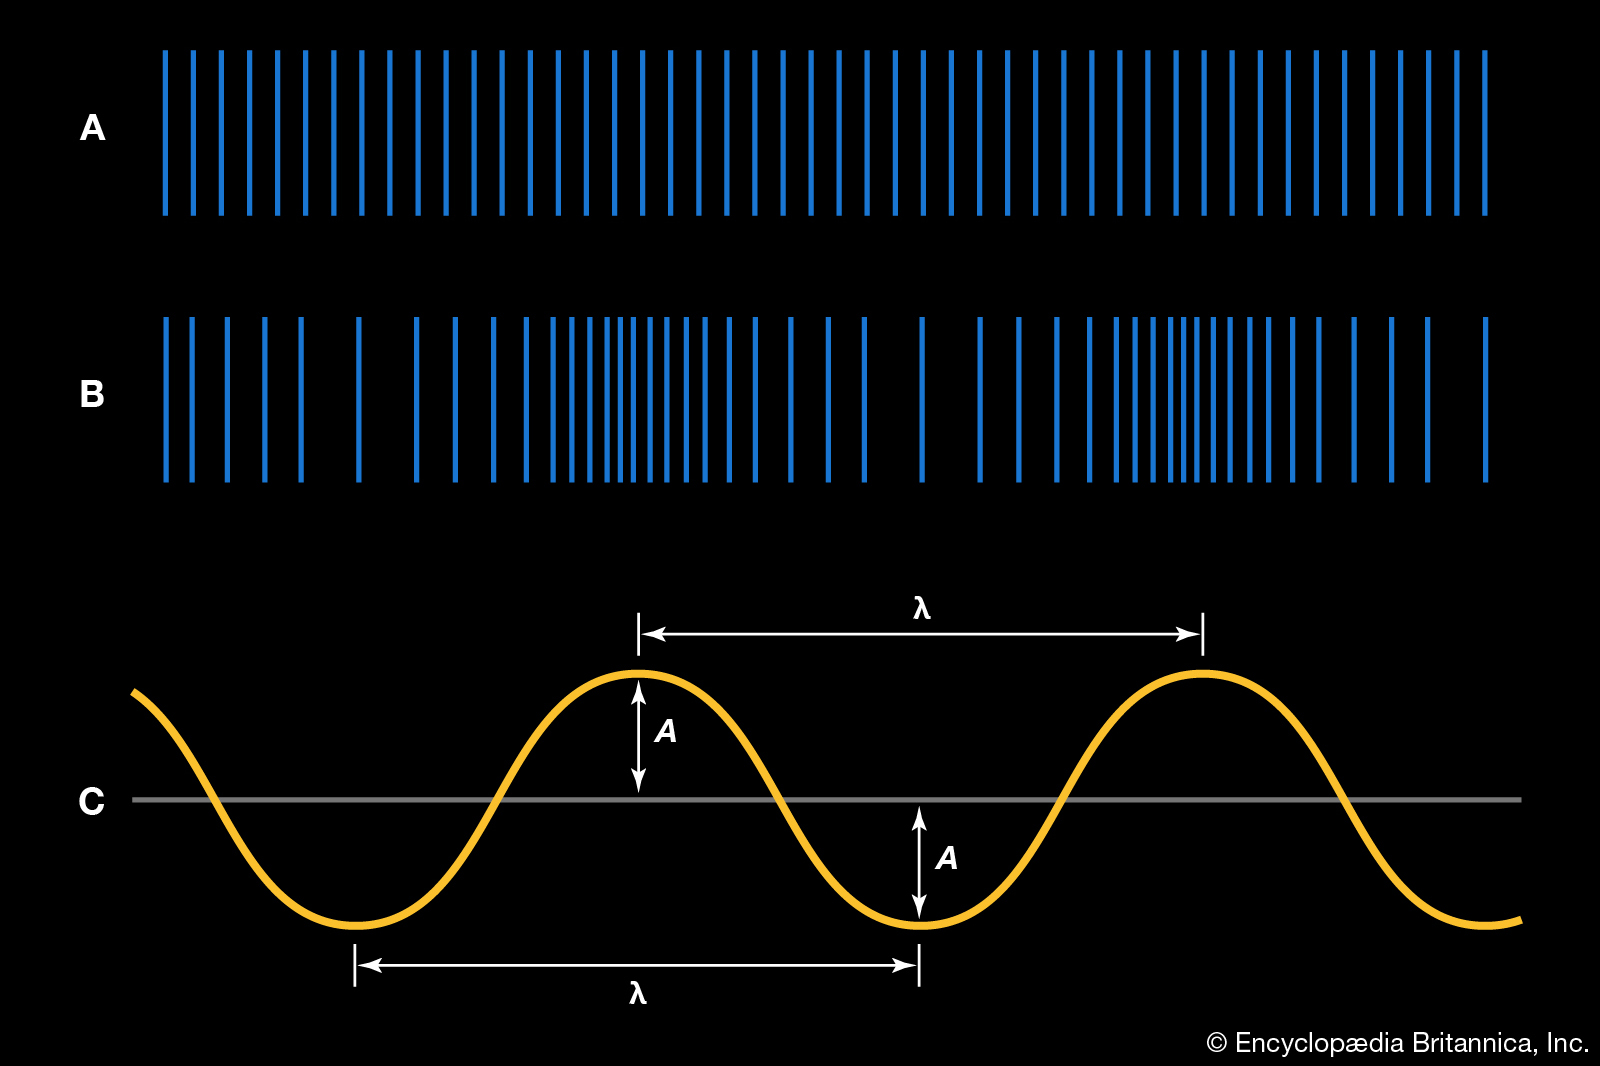
\includegraphics[scale=0.2]{img1.jpg}
    \caption{Représentations graphiques d’une onde sonore. (A) L’air à l’équilibre, avec l’absence de l’onde sonore. (B) compressions et réfractions qui constituent l’onde sonore. (C) Représentation graphique de l’onde sonore avec son amplitude A et sa longueur d’onde $\lambda$.}
\end{figure}

\subsection{Caractéristiques physique et description mathématique d’un signal sonore }

Il est important de remarque que dans figure précédente, plus précisément dans la partie C de cette figure, s’agit d’une autre représentation du signal sonore illustré dans la partie B. En effet, dans cette partie nous pouvons voire une courbe sinusoïdale, cette courbe représente la variation de la pression du signal sonore, celui-ci se répète de façon périodique. La distance entre 2 pics de la courbe est nommée longueur d’onde et se représente par la lettre $\lambda$. 

Lorsqu’un signal sonore ou onde sonore se déplace dans l’air, la longueur d’onde prend un certain temps pour aller d’un point $A$ à un point $B$ de l’espace, cette durée de temps est appelée période et note T. 

De plus, pendant un intervalle de temps équivalent à une seconde, un certain nombre de longueurs d’onde passe d’un point A à un point de l’espace. Ce phénomène est connu comme fréquence du signal. Dans d’autres mots, la fréquence est le nombre de périodes par unité de temps ce qui correspond à l’inverse de la période : $f=1/T$ ou f est la fréquence en Hertz ($Hz$ ou $s^-1$) et $T$ la période en seconde ($s$). 

Il est important de remarquer que les signaux sonores qui ont de hautes fréquences, ont des périodes courtes, alors que les signaux sonores qui ont des bases fréquences, ont de longs périodes. De plus, l’intervalle de fréquences que l’être humain peut percevoir se trouve entre les $20Hz$ et les $20 kHz$. Il existe une propriété physique qui permet de classifier les signaux sonores en fonction de la perception physiologique des êtres humains, cette propriété est connue comme le ton. En plus, les signaux ont une vitesse de déplacement, celle-ci est connue comme vitesse de l’onde ($S$), elle est obtenue par une relation entre la fréquence ou la période et la longueur d’onde, comme montrer ci-dessous : 

\[S = f*\lambda = \dfrac{\lambda}{T}\]

Le déplacement d’une onde sonore dans une dimension (signal sonore plat) est décrit mathématiquement par l’équation général du mouvement des ondes, qui peut être écrit de la façon suivante :  
 
\[y(x,t) = Asin(2\pi(ft - \dfrac{x}{\lambda}))\]

L'amplitude ($A$) d'une onde correspond à la hauteur maximale atteinte par l'onde par rapport à sa position n au repos. 

De plus, grâce à l’amplitude nous pouvons déterminer intensité de l’onde, qui est perçu par l’ouïe sous le nom de volume. L'intensité acoustique ($I$), est définie comme le taux de transmission d'énergie par unité d’aire perpendiculaire à la direction de propagation de l’onde. La relation existante entre l’intensité et l’amplitude est la suivante : 

\[I = \dfrac{A^2}{2\rho S}\]

Avec :

\begin{itemize} % Lista

    \item[-] $\rho$ : densité de l’air à l’équilibre (en $kg/m^3$).
    \item[-] $S$ vitesse de l’onde (en $m/s$).

\end{itemize}

L’intensité $I$ a pour unité les watt par mètre carré ($W/m^2$). Sous des “conditions atmosphériques standards, on a : 

\[\rho=10^5 Pa=10^5 \dfrac{N}{m^2}\]

L’amplitude minimum de variation de pression que l’ouïe humain peut percevoir es de $10^-5 Pa$ et l’amplitude maximal est de $10 Pa$. 

\subsection{Audition et perception du son chez les êtres humains}

D’après ce qui a été décrit précédemment, il est convenable de remarque les faits suivants :

\begin{itemize} % Lista

    \item[-] Entre $20 Hz et 20 kHz$ se trouve l’intervalle de fréquence perçu par l’être humain.  

    \item[-] L’amplitude d’une onde sonore permet de déterminer l’intensité de l’onde. 

    \item[-] L’amplitude minimum de variation de pression que l’ouïe humain peut percevoir es de $10^-5 Pa$ et l’amplitude maximal est de $10 Pa$.

\end{itemize}

\subsection{Echelles des décibels}

L’échelle des décibels est une échelle qui permet de classifie les ondes sonores en fonction de leur intensité sonore. Cette échelle est décrite par l’équation suivante : 

\[I_{dB} = L = 10log(\dfrac{I}{I_0})\]

Avec L qui représente les décibels, $I$ l’intensité de l’onde et $I_0=10^{-12}$ $W/m^2$ es l’intensité de référence. 

Plus précisément, L’échelle des décibels est logarithmique, ce qui signifie qu’une augmentation du niveau sonore de $3 dB$ représente déjà un doublement de l’intensité sonore. Par exemple, le volume d’une conversation normale peut être d’environ $65 dB$ et, pour quelqu’un qui crie, ce chiffre peut atteindre environ $80 dB$. La différence est seulement de $15 dB$, mais le cri représente une intensité trente fois supérieure. 

Le décibel ($dB$) est une unité utilisée pour mesurer l'intensité des sons et celle d'autres grandeurs physiques. Un décibel équivaut à un dixième de bel ($B$), une unité qui doit son nom à Graham Bell, l'inventeur du téléphone. Son échelle logarithmique permet de représenter le spectre auditif de l’être humain dans son ensemble.

% Imagen
\begin{figure}[H]
 \centering
    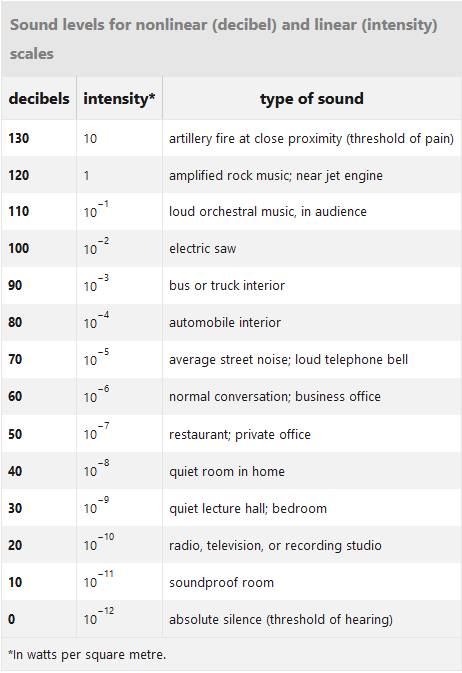
\includegraphics[scale=0.6]{img2.png}
\end{figure}

 Le champ auditif de l’être humain (en vert) est limité par une courbe qui nous fournis la limite inferieur et une autre courbe qui nous donne la limite supérieure de la perception sonore. A caque fréquence, entre $20 Hz et 20 kHz$, le seuil de notre sensibilité est différent. L’intervalle le plus large de perception a lieu aux alentours les $2 kHz$ et commence à partir des $0 dB$. Dans cet intervalle dit “moyen” les dynamiques sensorielles sont les plus aptes possibles et peuvent avoir un équivalent de $130 dB$.
 
% Imagen
 \begin{figure}[H]
 \centering
    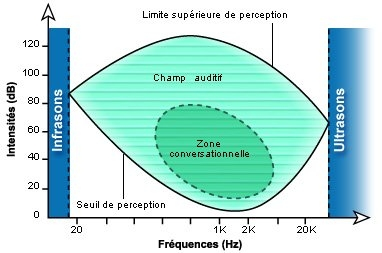
\includegraphics[scale=1.5]{img3.jpg}
    \caption{Courbe audiométrique de l'oreille humaine.}
\end{figure}

 \subsection{Tonalité pure}
 Lorsque nous utilisant de fonction comme celle de la vitesse de déplacement d’une onde, nous pouvons dire que cette fonction représente une tonalité pure avec un fréquence $f$. Ce nom dérive du fait que cette fonction décrit une onde sonore avec une seule composante en fréquence, c’est-à-dire qu’il s’agit d’un cas idéal, parce que en faisant analogie avec la lumière, dans la nature nous ne trouverons jamais une lumière monochromatique (d’une seule couleur, c’est-à-dire d’une seule fréquence), nous ne trouverons jamais une onde sonore avec cette caractéristique.  

Afin de donner une définition plus précise d’une tonalité pure, nous devons nous appuyer sur la définition donnée en psychoacoustique. En effet, en psychoacoustique, une tonalité pure, ou encore son pur ou note pure (en anglais : pure tone) est un son avec une forme d'onde sinusoïdale ; c'est-à-dire une onde sinusoïdale de n'importe quelle fréquence, phase et amplitude. En audiologie clinique, les tons purs sont utilisés pour l'audiométrie tonale (en) afin de caractériser les seuils d'audition à différentes fréquences. 

\subsection{Décomposition du son en tonalités propres}
Proprement dit, toute onde sonore résulte de l’addition de plusieurs tonalité pure de fréquence différente. La quantité de fréquence requise pour former le son $f$ correspond au contenue fréquentielle de $f$. N’importe lequel son peut être reconstruit en partant de son contenue fréquentielle. 

Une implémentation de ce qui est dit précédemment, n’importe-lequel son peut être considéré comme une fonction, peut être représenté par la somme de tonalités pures ou fonctions sinusoïdales, ce n’est pas une surprise que ça ait un lien avec le concept mathématique des Séries de Fourier. 

De plus, ce qu’on a vue précédemment implique aussi que le son $f$ peut être enregistrer en enregistrant tout simplement son contenue spectral.

\textbf{Remarque :} La série de Fourier  correspondante a une fonction $f(x)$ est définie par :
\begin{equation}
\frac{a_0}{2} + \sum_{n=1}^{\infty}(a_n\cos{\frac{nx\pi}{L}} + b_n\sin{\frac{nx\pi}{L}})
\end{equation}
Où les coefficients $a_n$ et $b_n$ sont appelés coefficients de Fourier et sont définies par :
\begin{equation}
    a_n = \frac{1}{L} \int_{-L}^{L}f(x)cos(\frac{nx\pi}{L})dx,\;
    b_n = \frac{1}{L} \int_{-L}^{L}f(x)sin(\frac{nx\pi}{L})dx
\end{equation}


\subsection{Spectre en fréquences}
Le spectre en fréquences montre les différentes fréquences présentes dans un son, c’est-à-dire, il montre le contenue fréquentiel qui caractérise le son et avec l’amplitude correspondante à chaque fréquence. Usuellement, il est présenté comme un graphique où on compare la fréquence avec l’intensité, la pression ou la puissance en $dB$. Il faut remarquer que la fréquence dominante (avec une amplitude plus grande que les autres) est connue comme fréquence fondamentale et le reste est connue comme harmoniques. Sur l’image ci-dessous, on peut observer le spectre en fréquence d’une flute qui joue la note G4 équivalente, approximativement, a une fréquence de $400 Hz$. Il est important de remarquer que la fréquence fondamentale c’est celle qui a la plus grande amplitude, les autres ce sont des harmoniques. Si on étudiait cette note dans un autres instrument musical, on obtiendra le même spectre en fréquence avec la même fréquence fondamentale , mais les harmoniques seraient différents. Cette dernière caractéristique explique pourquoi les êtres humains on perçoit chaque instrument d’une façon différente lorsqu’on joue une même note. Cette perception auditive est connue sous le nom de \underline{timbre}.

% Imagen
 \begin{figure}[H]
 \centering
    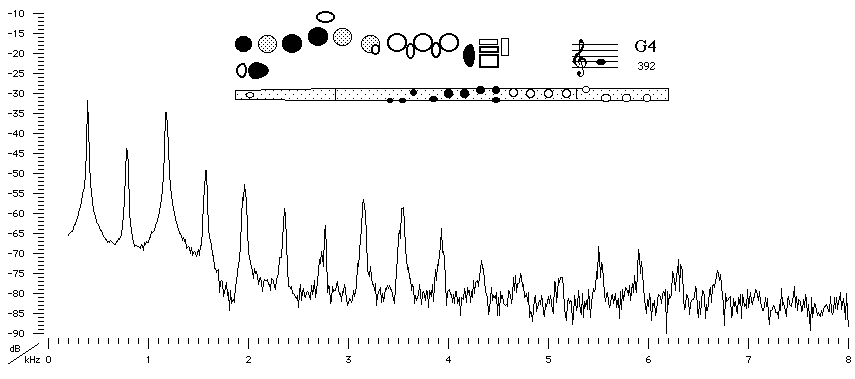
\includegraphics[scale=0.5]{img4.png}
    \caption{Spectre en fréquence du son d'une flute jouant la note G4 qui correspond, approximativement, à une fréquence de 400 Hz. On observe la fréquence fondamentale avec la plus grande amplitude et la présence des harmoniques}
\end{figure}

\subsection{Son digital}

L'échantillonnage d'un signal continu est l'opération qui consiste à prélever des échantillons du signal pour obtenir un signal discret, c'est-à-dire une suite de nombres représentant le signal, dans le but de mémoriser, transmettre, ou traiter le signal. 

L'échantillonnage intervient dans l'opération de conversion analogique-numérique, par exemple dans un dispositif de numérisation du son ou de l'image. Un autre exemple d'échantillonnage est celui que l'on fait pour obtenir la représentation graphique d'une fonction à une ou deux variables. D'une manière générale, l'échantillonnage intervient dans toute opération de conversion continu/discret. 

Le théorème de l'échantillonnage de Shannon, qui permet de savoir à quelle fréquence minimale il faut échantillonner un signal pour ne pas perdre l'information qu'il contient. 

Soit $u(t)$ une fonction représentant un signal continu. On considère un échantillonnage périodique défini par : 

\begin{equation}
    t_k = kT_e
    u_k = u(t_k)
\end{equation}

Où $k$ est un entier. $T_e$ est la période d'échantillonnage. $f_e=1/T_e$ est la fréquence d'échantillonnage. 

Le théorème de Shannon ([1]) concerne les signaux dont le spectre possède une fréquence maximale $f_{max}$, que l'on appelle des signaux à bande limitée. Par exemple, si $u(t)$ est un polynôme trigonométrique, la fréquence maximale est celle de la plus grande harmonique.

\textbf{Théorème de Shannon} : pour que le signal puisse être entièrement reconstruit à partir des échantillons, il faut et il suffit que : 

\begin{equation}
    f_e > 2f_max
\end{equation}

La fréquence d'échantillonnage doit être strictement supérieure à deux fois la plus grande fréquence présente dans le spectre du signal continu (condition de Nyquist-Shannon). Si cette condition est vérifiée alors : 

\begin{equation}
    u(t) = \sum_{k = -\infty}^{+\infty} u_k\sinc({\frac{t-kT_e}{T_e}})
\end{equation}

Où la fonction sinus cardinale est définie par : 

\begin{equation}
    \sinc{x} = \frac{\sin{(x\pi)}}{x\pi}
\end{equation}

Cette relation montre que le signal peut être reconstruit à partir des échantillons, ce qui signifie que toute l'information présente dans le signal original est conservée dans les échantillons. Nous verrons plus loin comment l'opération de reconstruction est effectuée en pratique. 

La moitié de la fréquence d'échantillonnage est appelée la fréquence de Nyquist $f_n$ et la condition de Nyquist-Shannon s'écrit donc $f_{max}<f_n$. 

Lorsque la condition n'est pas vérifiée, on dit qu'il y a sous-échantillonnage. On parle de sur-échantillonnage lorsque la fréquence de Nyquist est beaucoup plus grande que $f_max$. 

Le temps écoulé entre 2 échantillons successifs est connu comme période d’échantillonnage et est noté $T_s$. La longueur du vecteur est connue, usuellement, comme $N$ et a pour indices les numéros compris entre $0$ et $N-1$. Le processus de convertir une onde sonore(audio analogique) en un son digital est connue comme quantification de l’audio où à chaque échantillon on associe une valeur en amplitude (usuellement compris entre $-1$ et $1$). Le rand des possibles niveaux de l’amplitude, en d’autres mots,  le numéro d’échantillons équidistant de l’intervalle de valeurs d’amplitude $[-1, 1]$ est connue comme profondeur de couleur, par exemple :

\[8-bit = 2^8 = 256 \quad possibles valeurs\]
\[16-bit = 2^{16} = 65536 \quad possibles valeurs\]

Dans la figure ci-dessous, on peut observer l’effet de la quantification de l’audio et l’influence de la fréquence d’échantillonnage et la profondeur de couleur.

% Imagen
 \begin{figure}[H]
 \centering
    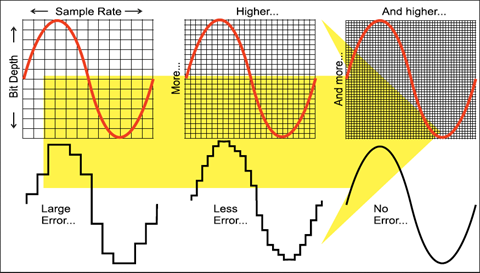
\includegraphics[scale=1]{img5.png}
    \caption{Quantification du son (audio analogique), influence de la fréquence d’échantillonnage (Sample Rate) et de la profondeur en couleur (Bit Depth). On observe que plus les paramètres sont grands, plus l’erreur sera grande.}
\end{figure}

Comme on peut voir dans la figure ci-dessus, la fréquence d'échantillonnage et la profondeur de couleur jouent un rôle fondamental dans la détermination de la qualité de l'audio résultant.

\subsection{Monophonique}
 Un son monophonique, enregistré ou écouté en mono (apocope de monophonie), dit aussi monaural, n'est diffusé que sur un seul canal comme provenant d'une seule source ou d'un seul endroit. Il est en général enregistré par un seul microphone et reproduit par un ou plusieurs haut-parleurs diffusant le même signal acoustique.
 
\subsection{Son stéréo}
Le son stéréophonique, plus communément appelé stéréo, est une méthode de reproduction sonore visant à reconstituer la répartition dans l'espace des sources d'origine1.

Ce relief sonore est habituellement obtenu à l'aide de deux canaux (gauche et droit) diffusés par au moins deux transducteurs (haut-parleurs ou écouteurs). Dans des conditions idéales, l'auditeur entend les sons comme dans la nature ou comme s'il était situé en face de l'orchestre lors d'un concert.

Le terme stéréophonie vient du grec Stéréo « spatial, solide » et phono « ton, le son ».

\subsection{Enregistrement d'un son digital sur un ordinateur}
Usuellement sur un ordinateur, on utilise la méthode de modulation par impulsions codifié (PCM, Pulse-code modulation en anglais) pour transformer un signal analogue en une séquence de bits (signal digital). Cette méthode a été inventé par Alec Reeves en 1937 et est la forme standard des enregistrement audios digital sur les ordinateurs
Pour qu’un ordinateur soit capable de reproduit un son digital, il faut que les échantillons obtenus soient sauvegardés dans un fichier ou dans la mémoire de l’ordinateur. Dans le cas du PCM, l’enregistrement se fait sous format RAW ou en autres types de format (WAV, AIFF, AU…). Néanmoins, comme les fichiers audios sont grand, ce qui est normal est de travailler avec des formats compressés qui réduisent la taille des fichiers.

\begin{itemize} % Lista

    \item[-] \textbf{formats avec des pertes} \textit{(lossy)}:  il s’agit de formats qui compressent le fichier original en éliminant des parties de celui-ci en suivant un algorithme de compression spécifique. De ce fait, lorsqu’on décompresse le fichier, on n’obtient pas le fichier original. Certains d’entre eux sont: \texttt{MP3, Opus, Vorbis, WMA,} etc.
    \item[-] \textbf{Formats sans pertes} \textit{(lossless)}: il s’agit du format qui compresse le fichier original en organisant l’information efficacement. De ce fait, lorsqu’on décompresse le fichier on obtient l’original. Certains d’entre eux sont : \texttt{FLAC, APE, WV, ALAC,} etc.

\end{itemize}

\subsection{Audio en Matlab}

Sur Matlab la lecture des audios se fait avec la fonction suivante :
\[\texttt{[y,Fs] = audioread('name.wav')}\]
Où
\begin{itemize}
    \item[] $\texttt{y}$ est une matrice de $m$ lignes et $n$ colonnes où $m=f*$\textit{durée} et $n$ est le nombres de canals de l’audio (avec 1 pour monophonique et 2 pour stéréophonique). Les valeurs enregistrer dans l’intervalle $[-1,1]$ correspondent a la representation de l’audio sur l’ordinateur. 
    \item[] $\texttt{Fs}$  est la fréquence d’échantillonnage de l’audio.
\end{itemize}
Sur Matlab l’écriture des audios se fait avec la fonction suivante :
\[\texttt{audiwrite('name.wav',y,Fs)}\]

\subsection{Bruit et types de bruit}
Comme vue précédemment, le bruit dans un signal sonore correspond à une perturbation de celui-ci entrainant des pertes de d’information. Il existe plusieurs types de bruit qui ont leurs propres domaines de fréquences et qui altèrent ou modifient l’information contenue dans un signal de façon différente. En effet, entre les différents types de bruits nous pouvons remarqués 2 groupes très importants : Les bruits dit naturels et les bruits dit industriels.  

Dans un premier temps, en regardant les bruits naturels nous pouvons nous rendre compte que ces bruits ne sont pas produits de façon artificielle et existe par différentes raisons. Dans cette famille de bruit nous pouvons trouvés le bruit ambiant qui correspond au bruit total existant dans une situation donnée pendant un intervalle de temps donné, ainsi que les bruits qui le compose telles que le bruit résiduel et le bruit particulier. De plus, nous trouvons aussi des bruits dis colorées telles que le bruit blanc ou le bruit rose, qui feront objet de notre étude de filtrage. Tout d’abord, il faut remarquer que le bruit blanc est un bruit composé par la somme de tous le bruit coloré, c’est à dire l’addition en fréquence du bruit rose, bruit rouge ou brownien, bruit bleu ou azur, bruit violet et bruit gris. Chacun d’entre eux aillant un domaine de fréquence particulier et des caractéristique propre. Par exemple :\\

 % Imagen
    \begin{figure}[H]
        \centering
        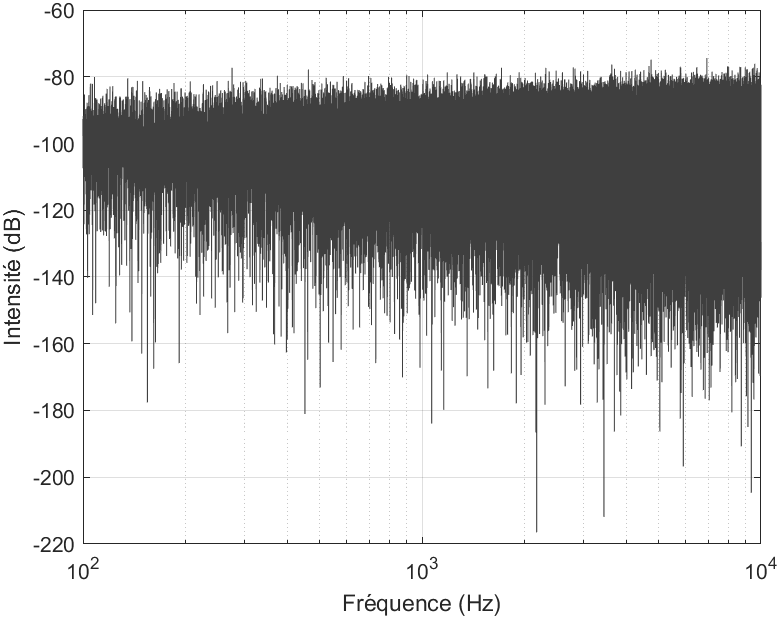
\includegraphics[scale=0.5]{img6.png}
        \caption{Spectre en fréquence du bruit blanc généré sur Matlab R2020a.}
    \end{figure}
    
\begin{itemize} % Lista

    \item[-] \textbf{Le bruit rouge ou brownien} correspond dans une première approximation, dans les domaines qui utilisent des définitions précises, la terminologie « bruit rouge », « bruit brownien » ou « bruit brun » fait référence au son ayant une puissance sonore qui décroît de 6 dB par octave lorsque la fréquence augmente (densité proportionnelle à $1/f$ ) sur un intervalle de fréquence n'incluant pas de DC (Qui dans un sens général, n'inclut pas de composante constante, ou de valeur pour $f=0$). 

    % Imagen
    \begin{figure}[H]
        \centering
        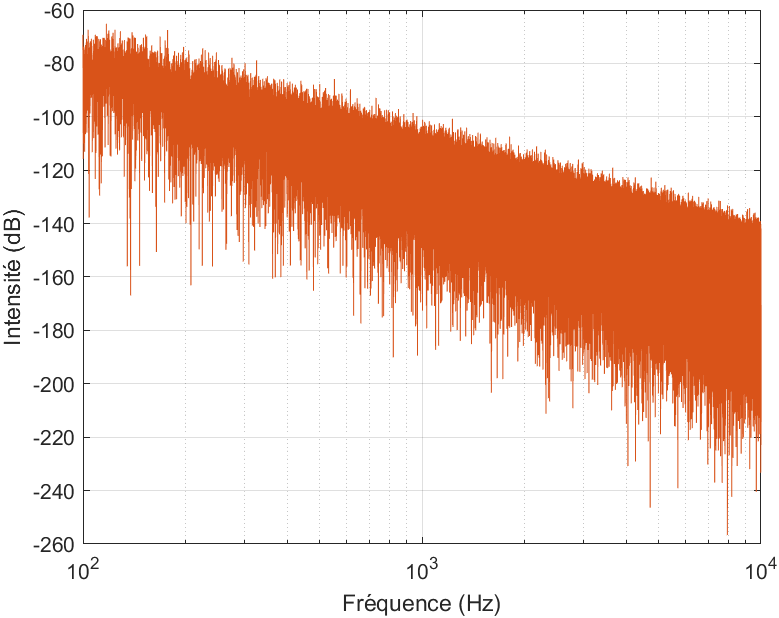
\includegraphics[scale=0.5]{img7.png}
        \caption{Spectre en fréquence du bruit rouge (-$6dB$/Octave) généré sur Matlab R2020a.}
    \end{figure}

    D’un autre point de vue, dans les domaines qui utilisent des définitions plus approximatives, le « bruit rouge » correspond à tout son dont la densité de puissance diminue lorsque la fréquence augmente. 

    Plus exactement Le bruit rouge, peut être obtenu en utilisant un algorithme simulant le mouvement brownien ou par intégration mathématique du bruit blanc.
    
    \item[-] \textbf{Le bruit rose} Le spectre sonore du bruit rose est plat dans un espace logarithmique. Ainsi, ce type de bruit est caractérisé par une puissance égale sur des bandes proportionnelles en largeur. Une bande correspond en fait à un changement de fréquence (hausse ou baisse à exprimer en pourcentage de l’une des extrémités de l’intervalle). Par exemple, la puissance d’un bruit rose est la même sur les intervalles allant de $40$ à $60 Hz$ et de $4 000$ à $6 000 Hz$ car ces intervalles sont proportionnels (ils correspondent à une hausse de 50\% de la fréquence).

    Or, l’appareil auditif humain est souvent étudié dans un espace logarithmique. En effet, l’oreille humaine ne perçoit les sons que sur des bandes de largeurs proportionnelles : un doublement de fréquence sera perçu en termes de puissance sonore de la même façon, quelle que soit la fréquence de départ. Ainsi, en musique, on a défini les octaves : une octave correspond à un doublement de fréquence et est perçu comme contenant la même puissance sonore. C’est pourquoi le bruit rose est souvent utilisé comme signal de référence en ingénierie du son.
    
    D’autre part, sur les diagrammes de spectres sonores, on voit que la densité de puissance sonore du bruit rose, comparée à celle du bruit blanc, diminue de $3dB$ par octave : la densité de puissance sonore est proportionnelle à $1/F$ (où $F$ est la fréquence). C’est pour cela que le bruit rose est souvent appelé « bruit $1/F$ ».
    
    % Imagen
    \begin{figure}[H]
        \centering
        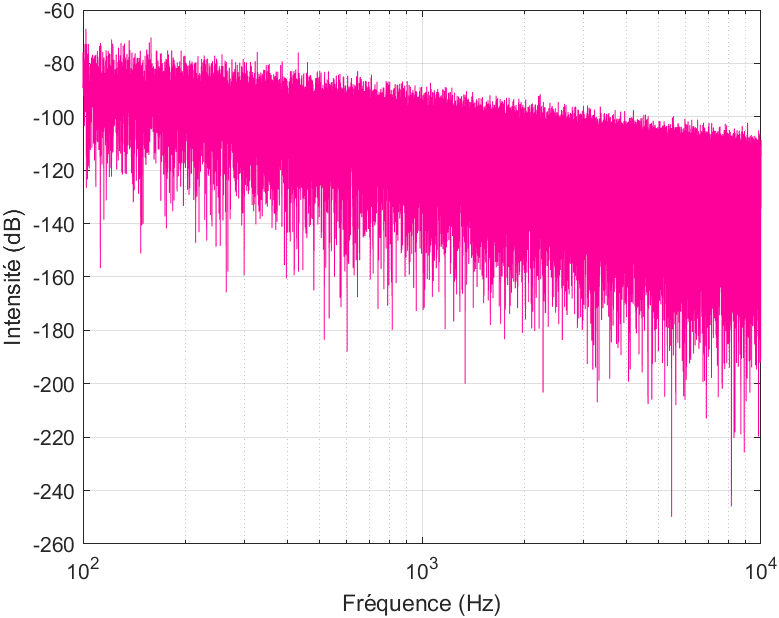
\includegraphics[scale=0.5]{img8.png}
        \caption{Spectre en fréquence du bruit rose (-$3dB$/Octave) généré su Matlab R2020a.}
    \end{figure}

    \item[-] \textbf{Le bruit bleu} qui correspond à un bruit qui augmente sa puissance sonore de $3dB$ par octave lorsque la fréquence augmente (densité proportionnelle à $f$), et ce jusqu’à une fréquence infinie. 

    Dans le domaine de l’informatique graphique, le terme « bruit bleu » est parfois utilisé d’une façon plus approximative pour décrire tout son de puissance sonore minimale à basse fréquence et ne présentant aucun pic lorsque la fréquence augmente (croissance constante). 

    Il est convenable de connaitre et différencier aussi le bruit rose des autres types de bruits coloré, dans la mesure que ce type de bruit fait partie de notre étude. Donc le bruit rose, ce type de bruit est caractérisé par une puissance égale sur des bandes proportionnelles en largeur. Une bande correspond en fait à un changement de fréquence (hausse ou baisse à exprimer en pourcentage de l’une des extrémités de l’intervalle). Par exemple, la puissance d’un bruit rose est la même sur les intervalles allant de $40$ à $60Hz$ et de $4000$ à $6000Hz$ car ces intervalles sont proportionnels (ils correspondent à une hausse de 50 pourcent de la fréquence). 

\end{itemize}
\hfill

Dans un deuxième temps, nous voyons l’existence d’une deuxième
famille de bruits que nous choisissant de nommé des bruits
industriels. En effet, comme son nom l’indique les bruits
industriels sont des perturbations sonores produits par l’industrie
ou par des effet industrie. Dans cette famille nous trouvons des
bruits tels que le bruit de route qui est un bruit normalisé. Il est
une référence pour le bruit des trafics routiers et ferroviaires.
Son spectre est enrichi en basses fréquences et appauvri dans les
aiguës par rapport à un bruit rose. Mais aussi nous trouvons des
bruits comme les suivants :
\hfill

\begin{itemize}

    \item[-] \textbf{Le bruit d’impact}: c’est le bruit transmis par une paroi mise en vibration par un choc (bruit de pas, déplacement de meubles, chute d’objet, enfoncement d’un clou dans un mur...).
    \item[-] \textbf{Le bruit aérien}: c’est le bruit propagé dans l’air (bruit de voix, bruit de télévision, bruit de circulation...). 
    \item[-] \textbf{Le bruit solidien}: c’est le bruit propagé dans les milieux solides comprenant (le bruit d’impact transmis par les éléments solides, le bruit d’équipement (chaufferie, ascenseurs, ...). 
    
\end{itemize}

\newpage
\section{Méthodes}
Le but de ce projet est d’implémenter le filtrage dans les notes audios dans l'objectif d'atténuer le bruit présent. Pour cela nous allons implémenter le filtrage analogique avec une approximation de Butterworth, la méthode RNN et un autre qui reste définir.

\subsection{\textbf{Filtre de Butterworth}}

\subsubsection{définition du filtrage}
\medskip
Le filtrage est une forme de traitement de signal, obtenu en envoyant le signal à travers un ensemble de circuits électroniques, qui modifient son spectre de fréquence et/ou sa phase et donc sa forme temporelle. Il peut s‘agir soit : 

\begin{itemize}
    \item[-] d’éliminer ou d’affaiblir des fréquences parasites indésirables 

    \item[-] d’isoler dans un signal complexe la ou les bandes de fréquences utiles. 
\end{itemize}

Il existe plusieurs types de filtres : passe-bas, passe-haut, passe-bande, coupe-bande, réjecteur de bande. Dans notre étude, nous allons nous concentrer dans les filtres passe-bas.

\medskip
\subsubsection{Filtre passe-bas}
Un filtre passe-bas est un filtre qui laisse passer les basses fréquences et qui atténue les hautes fréquences, c'est-à-dire les fréquences supérieures à la fréquence de coupure. Il pourrait également être appelé filtre coupe-haut. Le filtre passe-bas est l'inverse du filtre passe-haut et ces deux filtres combinés forment un filtre passe-bande. 

Un filtre passe-bas peut être implémenté de façon analogique avec des composants électroniques. Ainsi, ce genre de filtre s'applique sur des signaux continus en temps réel. Les composants et la configuration du circuit fixeront les différentes caractéristiques du filtre, telles que l'ordre, la fréquence de coupure et son diagramme de Bode. Les filtres analogiques classiques sont du premier ou du second ordre. Il existe plusieurs familles de filtres analogiques : Butterworth, Tchebychev, Bessel, elliptique, etc. L'implémentation des filtres de même famille se fait généralement en utilisant la même configuration de circuit, et ceux-ci possèdent la même forme de fonction de transfert, mais ce sont les paramètres de celle-ci qui changent, donc la valeur des composants du circuit électrique.
\medskip

\paragraph{Filtre passe-bas du premier ordre}
Un filtre passe-bas du premier ordre est caractérisé par sa fréquence de coupure $f(c)$.  La fonction de transfert du filtre est obtenue en dénormalisant le filtre passe-bas normalisé en en remplaçant $\omega_n$ par $\omega$, $\omega_c$,
Ce qui donne la fonction de transfert suivante :

\begin{equation}
    H(j\omega)= \frac{v_o}{v_i} = \frac{K}{1+j\frac{\omega}{\omega_c}}
\end{equation}

Où
\begin{itemize}
    \item[] $v_i$ est le signal d'entrée
    \item[] $v_0$ est le signal de sortir
\end{itemize}


Le module et la phase de la fonction de transfert sont égaux à :

\begin{equation}
    |H(\omega)|=|\frac{v_o}{v_i}|= \frac{K}{\sqrt{1 + (\frac{\omega}{\omega_c})^2}}
\end{equation}

\begin{equation}
    \phi(\omega) = arg(H(j\omega)) = -arg(1 + j\frac{\omega}{\omega_c}) = \arctan(\frac{\omega}{\omega_c})
\end{equation}

Il y a plusieurs méthodes pour implémenter ce filtre. Une réalisation active et une réalisation passive sont ici présentées. $K$ est le gain du filtre.

\paragraph{Circuit actif}
\hfill\\
Il est  possible de réaliser un filtre passe-bas avec un circuit actif. Cette option permet d'ajouter du gain au signal de sortie, c'est-à-dire d'obtenir une amplitude supérieure à $0dB$ dans la bande passante. Plusieurs configurations permettent d'implémenter ce genre de filtre.

%imagen
 \begin{figure}[H]
 \centering
    \includegraphics[scale=0.5]{Circuit.png}
    \caption{Un filtre passe-bas actif}
\end{figure}

Un filtre passe-bas actif
Dans la configuration présentée ici, la fréquence de coupure se définit comme suit :

\begin{equation}
    f_c = \frac{1}{2\pi R_2C} 
\end{equation}

Où  
\begin{equation}
    \omega_c = \frac{1}{R_2 C}
\end{equation}

En utilisant les propriétés des amplificateurs opérationnels, et les impédances des éléments, on obtient la fonction de transfert suivante :

\begin{equation}
    H(j\omega)= \frac{v_o}{v_i} = \frac{-R_2}{R_1} \cdot \frac{1}{1 + jR_2 C\omega}
\end{equation}

En basse fréquence, le condensateur agit comme un circuit ouvert, ce qui est confirmé par le fait que le terme de droite de l'équation précédente tend vers $1$. La formule simplifiée ainsi obtenue nous donne le gain dans la bande passante :

\begin{equation}
    H(\omega)_{\omega \ll \omega_c}  = \frac{v_o}{v_i} = \frac{-R_2}{R_1}
\end{equation}


Avec la fonction de transfert, on peut démontrer que l'atténuation dans la bande rejetée est de $20 dB/$\textit{décade} ou de $6dB$ par octave telle qu'attendu pour un filtre d'ordre $1$.
\medskip

\paragraph{Filtre passe-bas du second ordre}
\hfill\\
Un filtre passe-bas du second ordre est caractérisé par sa fréquence propre $f_0$ et par un facteur de qualité $Q$.  Il est représenté par la fonction de transfert suivante :


\begin{equation}
    H(j\omega) = \frac{v_o}{v_i} = \frac{K}{1 - (\frac{\omega}{\omega_0})^2 + j\frac{(\omega/\omega_0)}{Q}}
\end{equation}

Avec
\begin{itemize}
  \item[] $\omega =  2\pi f$
  \item[] $\omega_0 = 2\pi f_0$ 
\end{itemize}


Le module et la phase de la fonction de transfert sont donc donnés par:

\begin{equation}
    |H(j\omega)| = |\frac{v_o}{v_i}| = \frac{K}{\sqrt{(1 - (\frac{\omega}{\omega_0})^2)^2 + (\frac{(\omega/\omega_0)}{Q})^2}}
\end{equation}

\begin{equation}
    \phi(\omega) = -arctan\left(\frac{\frac{(\omega/\omega_0)}{Q}}{1 - (\omega/\omega_0)^2})\right)
\end{equation}

\subsubsection{Types de Filtres Analogiques Passe-bas}
\paragraph{Approximation de Butterworth}
\hfill \\
Un filtre de Butterworth est un type de filtre linéaire, conçu pour posséder un gain aussi constant que possible dans sa bande passante.

Les filtres de Butterworth furent décrits pour la première fois par l'ingénieur britannique Stephen Butterworth

\begin{itemize}
  \item[-] \textbf{Caractéristiques}
  Le gain d'un filtre de Butterworth est le plus constant possible dans la bande passante et tend vers 0 dans la bande de coupure. Sur un diagramme de Bode logarithmique, cette réponse décroît linéairement vers -$\infty$, de -$6dB/octave$ (-$20 dB/$\textit{décade}) pour un filtre de premier ordre, -$12dB/octave$ soit -$40dB/$\textit{décade} pour un filtre de second ordre, -$18dB/octave$ soit -$60dB/4$\textit{décade} pour un filtre de troisième ordre, etc.
  
  %Imagen
  \begin{figure}[H]
 \centering
    \includegraphics[scale=0.5]{Filter.jpeg}
    \caption{Gains de filtres de Butterworth passe-bas d'ordre $1$ à 5 en fonction de la fréquence}
\end{figure}
  
  \item[-] \textbf{Fonction de Transfert}
  Le gain d'un filtre de Butterworth passe-bas d'ordre n est :
  
  \begin{equation}
      G_n(\omega) = |H(j\omega)| = \frac{1}{\sqrt{1 + (\frac{\omega}{\omega_0})^2}}
  \end{equation}

\end{itemize}

Avec
\begin{itemize}
    \item[] $G_n$ est le gain du filtre.
    \item[] $H_n$ sa fonction de transfert.
    \item[] $j$ l'unité imaginaire $j^2 = -1$
    \item[] $\omega$ la fréquence angulaire (ou pulsation) du signal en radians par seconde ($\omega = 2\pi f$)
    \item[] et $\omega_c$ la fréquence de coupure (angulaire) du filtre (à -$3dB$).
\end{itemize}
En normalisant l'expression (c’est-à-dire en spécifiant $\omega_c = 1$):

\begin{equation}
    G_n(\omega) = |H(j\omega)| = \frac{1}{\sqrt{1 + \omega}^2}
\end{equation}

Les $2n-1$ premières dérivées de $G_n$ sont nulles pour $\omega = 0$, impliquant une constance maximale du gain dans la bande passante.

Aux hautes fréquences :

\begin{equation}
    |H(j\omega)|_{dB} \approx -20 \cdot n\log_{10}(\omega)
\end{equation}
Le roll-off du filtre (la pente du gain dans un diagramme de Bode) est de $-20n$ $dB/$\textit{décade}, où 'n' est l'ordre du filtre.

Le gain ne représente que le module de la fonction de transfert $H(p)$ (au sens de la transformée de Laplace), ce qui laisse une certaine latitude pour déterminer cette dernière. On doit avoir

\begin{equation}
    H(p)H(-p) = \frac{G_0^2}{1 + (-\frac{p^2}{\omega_c^2})^n}
\end{equation}

Les pôles de cette expression sont équirépartis sur un cercle de rayon  $\omega_c$. Pour que le filtre soit stable, on choisit les pôles de la fonction de transfert comme ceux de $H(p)H(-p)$ ayant une partie réelle négative. Le k-ième pôle est donné à l'aide des racines nièmes de l'unité :

\begin{equation}
    -\frac{p_k^2}{\omega_k^2} = \exp({\frac{j(2k - 1)\pi}{n}}); k = 1,2,3, ...,n
\end{equation}
    

D’où

\begin{equation}
    p_k = \omega_c\exp{\frac{j(2k + n - 1)\pi}{2n}};  k = 1,2,3, ...,n
\end{equation}

La fonction de transfert s'écrit en fonction de ces pôles :

\begin{equation}
    H(p) = \frac{G_0}{\prod{n=1}^{n}\frac{(p - p_k)}{\omega_c}}
\end{equation}

Le polynôme au dénominateur est appelé polynôme de Butterworth.

\begin{center}
    \begin{tabular}{|| c c||}
    \hline
    n & Polynôme de Butterworth $B_n(p)$ pour $w_c = 1$ \\ [0.5ex]
    \hline \hline
    1 & $(p + 1)$ \\
    \hline
    2 & $p^2 1.4142p + 1$ \\
    \hline
    3 & $(p + 1)(p^2 + p + 1)$ \\
    \hline
    4 & $(p^2 + 0.7654p + 1)(p^2 + 1.8478p + 1)$ \\
    \hline
    5 & $(p + 1)(p^2 + 0.6180p + 1)(p^2 1.6180p + 1)$ \\
    \hline
    6 & $(p^2 + 0.5176p + 1)(p^2 + 1.4142p + 1)(p^2 + 1.9319p + 1)$ \\
    \hline
    7 & $(p + 1)(p^2 0.4450p 1)(p^2 + 1.2470p + 1)(p^2 + 1.8019p + 1)$ \\
    \hline
    8 & $(p^2 + 0.3902p + 1)(p^2 + 1.1111p + 1)(p^2 + 1.6629p + 1)(p^2 + 1.9616 + 1)$ \\ [0.1ex]
    \hline
    \end{tabular}
\end{center}




Les polynômes normalisés de Butterworth peuvent être utilisés pour déterminer les fonctions de transfert de filtre passe-bas pour toute fréquence de coupure $\omega_c$ selon que:

\begin{equation}
    H(p) = \frac{G_0}{B_n(a)}, a = \frac{p}{\omega_c}
\end{equation}

\paragraph{Approximation de Tchebychev}
\hfill
\medskip
\begin{itemize}
    \item[-] \textbf{Fonction de Transfert:}
    Les filtres Tchebychev de type I sont les types les plus courants de filtres Tchebychev. La réponse en gain (ou en amplitude) , en fonction de la fréquence angulaire du filtre passe-bas du n ième ordre est égale à la valeur absolue de la fonction de transfert évaluée à $G_n(s)\omega H(s)s = j\omega$

        \begin{equation}
            G_n(s) = |H_n(j\omega)| = \frac{1}{\sqrt{1 + \epsilon^2T_n^2(\frac{\omega}{\omega_0})}}
        \end{equation}

        Où $\epsilon$ est le facteur d'ondulation,$\omega_0$ est la fréquence de coupure et $T_n$ est un polynôme de Tchebychev du $n$-ème ordre
    
        \item[-] \textbf{Polynôme de Tchebychev:}
        La définition classique des polynômes de Tchebychev de première espèce est le plus souvent donnée par la relation de récurrence suivante :

            \begin{equation}
                T_{n+1} = 2XT_n - T_{n1}; \forall n \geq 0; T_0 = 1;  T_1 = X
            \end{equation}
 
\end{itemize}


\paragraph{Filtre de Bessel}
\hfill
\medskip
\begin{itemize}
    \item[-] \textbf{Fonction de Transfert:}
    Un filtre passe-bas Bessel se caractérise par sa fonction de transfert :

        \begin{equation}
            H(s) = \frac{\Theta_n(0)}{\Theta_n(s/\omega_0)}
        \end{equation}

    Où $\Theta_n(s)$ est un polynôme de Bessel inversé dont le filtre tire son nom et $\omega_0$ est  la fréquence de coupure . Le filtre a un retard de groupe basse fréquence de $1/\omega_0$. Puisque est indéterminé par la définition des polynômes de Bessel inversés, mais $\Theta_n(0)$ est une singularité amovible, il est défini que $\Theta_n(0) =  \lim_{x\to\infty} \Theta_n(x)$

    \item[-] \textbf{Polynôme de Bessel:}
        Les polynômes de Bessel inversés sont donnés par: 

        \begin{equation}
            \Theta_n(s) =  \sum_{k=0}^{n} a_k s^k 
        \end{equation}

        Où

        \begin{equation}
            a_k = \frac{(2n - k!)}{2^{n-k} k!(n-k!)}; k = 1,2,3, ...,n
        \end{equation}
\end{itemize}

\subsubsection{Notions Importantes}
\paragraph{Diagramme de Bode}
Le diagramme de Bode d'un système de réponse fréquentielle $T(j\omega)$ se compose de deux tracés:

\begin{itemize}
    \item[-] le gain (ou amplitude) en décibels (dB). Sa valeur est calculée à partir de $20\log_{10}(|T(j\omega|)$

    \item[-] la phase en degré, donnée par $arg(T(j\omega))$
\end{itemize}

L'échelle des pulsations est logarithmique et est exprimée en rad/s (radian par seconde). L'échelle logarithmique permet un tracé très lisible, car construit à partir de tronçons de ligne droite.

%imagen
%diagramme de Bode
\begin{figure}[H]
 \centering
    \includegraphics[scale=0.3]{Bode.jpeg}
\end{figure}

\paragraph{Transformée de Laplace}
La transformée de Laplace d’une fonction $f(t)$ est :
\begin{equation}
    F(s) = L{f(t)} = \int\limits_{0}^{\infty}\ f(t)\exp(-st) dt
\end{equation}

La transformée de Laplace permet de transformer le problème du domaine du temps au domaine de fréquence.
Lorsqu’on obtient la réponse voulue dans le domaine de fréquence, on transforme le problème á nouveau dans le domaine du temps, á l’aide de la transformée inverse de Laplace, qui est définie par:

\begin{equation}
    f(t) = L^{-1}{F(s)} = \frac{1}{2j\pi} \int\limits_{-\infty}^{\infty} \ F(s)\exp(st) ds
\end{equation}

\subsubsection{Implémentation de filtre de Butterworth sur Matlab}

\paragraph{Fonction Matlab Butter}
\hfill \\
Lorsqu’on a  effectué les recherches documentaires sur le filtre passe bas de Butterworth, on s’est rendu compte que le logiciel Matlab comptait déjà avec une fonction qui permet de créer ce filtre. De même, il compte avec d’autres fonctions permettant de créer les filtres analogiques vue précédemment. La fonction correspondante au filtre passe-bas avec une approximation de Butterworth est la suivante :

\[\texttt{butter}\]

\textbf{Remarque :} La fonction \textit{butter} permet de créer des filtres passe-bas, passe-haut, coupe bande et réjecteur de bande. Le type de filtre qu’elle créera est spécifié comme un paramètre.
  
La fonction \textit{butter} est bien intéressante dans la mesure où elle peut être utilisé de $5$ façons différentes, c’est-à-dire qu’il s’agit d’une fonction polymorphique. 

La première façon de l’utilisé est la suivante


\[\texttt{[b,a] = butter}(\texttt{n},\omega_\texttt{n})\]

Elle revoit les coefficients de la fonction de transfert d’un filtre digital passe-bas de Butterworth d’ordre $n$ et avec une fréquence de coupure normalisé $\omega_n$. 

La deuxième façon est la suivante :

\[\texttt{[b,a] = butter}(\texttt{n},\omega_\texttt{n}, \texttt{ftype})\]

Elle renvois les coefficients de la fonction de transfert comme précédemment, mais cette manière d’utilisé la fonction butter permet de définir le type de filtre qui est rentré dans le paramètre \texttt{ftype}. \textbf{Remarque :} Les filtres résultants lors de la création d’un coupe band ou réjecteur de bande son de l’ordre de $2n$.

La troisième façon est :

\[\texttt{[z,p,k] = butter}(\_\_\_)\]

Cette utilisation de la fonction butter, conçoit un filtre de Butterworth passe-bas, passe-haut, coupe bade ou réjecteur de bande et renvois les zéros, les pôles et le gain du filtre. Cette syntaxe peut recevoir n’importe lequel argument d’entrée de ceux qu’on a vue précédemment.
La quatrième est :

\[\texttt{[A,B,C,D] = butter}(\_\_\_)\]

Cette utilisation , conçoit un filtre de Butterworth passe-bas, passe-haut, coupe bade ou réjecteur de bande et renvois ses matrices de représentation spatiale dans son état actuel.
Et la cinquième et dernière :

\[\texttt{[\_\_\_] = butter}(\_\_\_,\texttt{'s'})\]

Conçoit un filtre analogique de Butterworth passe-bas, passe-haut, coupe bade ou réjecteur de bande avec une pulsation ou fréquence angulaire de coupure $\omega_n$.

On s’intéresse à la première syntaxe de la fonction \texttt{butter}.

Pour créer notre filtre passe-bas de Butterworth, il faut qu’on définisse la fréquence de sortie, la fréquence de coupure et l’ordre du filtre. 
On définit ses paramètres de la façon suivante sur la ligne de code Matlab :

\[\texttt{fs = }60000 \texttt{;}\]
\[\texttt{fc = }1000 \texttt{;}\]
\[\texttt{n = }2 \texttt{;}\]

Où \texttt{fs} es la fréquence de sortie, \texttt{fc} est la fréquence de coupure et $n$ est l’ordre du filtre. 
Puis, on rentre la ligne de code suivante :

\[\texttt{[pôles, zéros] = butter}(\texttt{n,fc/(fs/2)}) \texttt{;}\]

Et Matlab nous revoit :
\begin{figure}[H]
 \centering
    \includegraphics[width=0.7\textwidth]{nuevobutter1.png}
\end{figure}

On a maintenant les pôles et les zéros de notre filtre passe-bas de Butterworth, mais on veut aussi voir à quoi il ressemble ou plutôt à quoi ressemble son diagramme de Bode en gain et phase. Pour cela, on rentre sur la ligne de code de Matlab, la commande suivante :

\[\texttt{ freqz(poles,zeros)}\]


Matlab nous revoit le graphique ci-dessous :

\begin{figure}[H]
 \centering
    \includegraphics[width=0.7\textwidth]{nuevobutter2.png}
    \caption{Diagramme de Bode en gain et en phase du filtre de Butterworth d'ordre 2 et de fréquence de coupure $f_c = 1000 Hz$.}
\end{figure}

\paragraph{Importation du filtre de Butterworth sur l'outil sptool}
\hfill \\

L'outil \textit{sptool} est un outil Matlab qui permet l'analyse, la visualisation et le traitement des signaux. Lorsqu'on verra la modification de la méthode du filtre de Butterworth, on expliquera plus en détail l'utilisation de cet outil. Dans cette partie on se limitera à montrer comment importer les pôles et les zéros corresponds au filtre pour ainsi pour créer le filtre dans cet outil, et par la suite pourvoir l'utiliser dans le filtrage des signaux en question.

Tout d’abord, on ouvre l’outil \textit{sptool} en rentrant sur la ligne de code la commande suivante :
\[\texttt{sptool}\]

Matlab nous ouvrira la fenêtre ci-dessous correspondante a l’outil \textit{sptool} :

 \begin{figure}[H]
 \centering
    \includegraphics[scale=0.3]{b5.jpeg}
    \caption{Outil Matlab sptool}
\end{figure}


Puis on clique sur l’onglet \textit{File} et on choisir l’option \textit{Import…}, comme le montre l’image ci-dessous :

 \begin{figure}[H]
 \centering
    \includegraphics[scale=0.7]{nuevobutter13.png}
\end{figure}

Ensuite, une nouvelle fenêtre s’ouvre où on peut importer les vecteurs correspondants pôles et zéros dans le but de créer notre filtre dans l’outil \textit{sptool}. Tout d’abord, on choisit sur la colonne \textit{Source} l’endroit d’où en importera les vecteurs, dans ce cas coche l’option \textit{From Workspace}. Puis dans la colonne \textit{Import As :}, on choisit \textit{Filter} sur l’option déroulante, qui se trouve à cote du label \textit{Import As :}, et on confirme que l’option \textit{Tranfer Function} soit choisi dans l’option déroulante qui se trouve à cote du label \textit{Form : }. On remarque entre les colonnes \textit{Workspace Contents} et la colonne \textit{Import As : }, qui vient de changer, apparaissent 2 petits flèches qui pointe ver la colonne \textit{Import As : }. Ces 2 flèches illustrent l’importation des vecteurs correspondants aux pôles et aux zéros de la fonction de transfert du filtre. Ensuite en sélection le vecteurs \textit{zéros} et cliquant sut la flèche qui pointe vers le label \textit{Numerator} et on fait de même avec le vecteur \textit{pôles} et la flèche qui pointe vers le label \textit{Denominator}. Puis sur la ligne \textit{Name} qui se trouve en bas de la colonne \textit{Import As : }, on définit le nom de notre filtre, dans ce cas on nomme notre filtre comme \textit{filtbutter1}. L’image ci-dessous illustre cette procédure.

 \begin{figure}[H]
 \centering
    \includegraphics[scale=0.6]{nuevobutter4.png}
\end{figure}

Puis, on clique sur le buton \textit{OK} et on crée notre filtre. On revient alors sur la fenêtre principale de \textit{sptool} et on remarque qu'il y a un nouveau filtre sur la colonne \textit{Filters} (voir image ci-dessous).

\begin{figure}[H]
 \centering
    \includegraphics[scale=0.6]{nuevobutter5.png}
\end{figure}

Maintenant, si on veut voir l'allure du diagramme de Bode de notre filtre, il suffira de le sélectionner et de cliquer sur le buton \textit{View}, comme le montre l'image ci-dessous.

\begin{figure}[H]
 \centering
    \includegraphics[scale=0.6]{nuevobutter6.png}
\end{figure}

Il nous renvois une nouvelle fenêtre sur laquelle on peut voir le diagramme de Bode en gain, le diagramme de Bode en phase ou les 2 diagrammes de Bode dans un seul graphique. On choisit la dernière option (voir image ci-dessous) et remarque qu'il s'agit du même diagramme de Bode que celui qu'on a vue dans le paragraphe \textit{Fonction Matlab butter}, ce qu’est normal.

\begin{figure}[H]
 \centering
    \includegraphics[scale=0.7]{nuevobutter7.png}
    \caption{Diagramme de Bode en gain et phase du filtre}
\end{figure}

\paragraph{Filtrage avec l'outil sptool}
\hfill \\ 

Pour effectuer le filtrage des signaux en question, on utilisera aussi l’outil \textit{sptool}. Dans la partie \textit{Butterworth modifiée}, plus précisément dans le paragraphe \textit{ Modification du filtre de Butterworth à partir de la fréquence de coupure}, on expliquera plus en détail l’importation d’un signal dans l’outil \textit{sptool}.

Dans cette partie, on se limitera à expliquer comment filtrer avec notre filtre, un signal déjà importe dans l’outil. Tout cela pour éviter la répétition d’une explication qui pourrait entrainer à une confusion. 

Après avoir importé le signal dans l’outil \textit{sptool}, on remarque que sur la colonne \textit{Signals}, on a un nouveau signal nommé \textit{original} (voir image ci-dessous). 

\begin{figure}[H]
 \centering
    \includegraphics[scale=0.6]{nuevobutter10.png}
\end{figure}

Matlab nous renvois une nouvelle fenêtre où on put définir le nom du nouveau signal. On choisit de le nommé \textit{sig1}. (Voir image ci-dessous).

\begin{figure}[H]
 \centering
    \includegraphics[scale=0.6]{nuevobutter11.png}
\end{figure}

Puis en cliquant sur le buton \textit{OK}. Matlab nous renvois le graphique ci-dessous correspondant au spectre en fréquence du nouveau signal.

\begin{figure}[H]
 \centering
    \includegraphics[scale=0.6]{nuevobutter9.png}
    \caption{Spectre en fréquence su signal filtré.}
\end{figure}

Maintenant, on exporte le nouveau signal dans le \textit{Workspace} en cliquant sur l’onglet \textit{File} et en choisissant l’option \textit{Export…}. Une fois le signal exporter, on constate que le vecteur qui nous intéresse est compris dans la structure \textit{sig1}. Pour récupérer ce vecteur, on rentre la ligne de commande suivant :

\[\texttt{y1 = sig1.data ;}\]

Et on remarque qu’un nouveau vecteur est définit sur notre \textit{Workspace}. 

A partir de ce vecteur et de la variable f, on crée un nouveau fichier audio avec la fonction \textit{audiowrite} (l’explication de l’utilisation de cette fonction se trouve dans partie  \textit{Butterworth modifiée}, plus précisément dans le paragraphe \textit{ Modification du filtre de Butterworth à partir de la fréquence de coupure}). Puis nous effectuant une comparaison du taux de bruit présent dans le signal, en utilisant une analyse statistique, ce que nous permet d’obtenir les tableaux de la partie \textit{Résultats Quantitatifs}. On effectue cette même procédure pour les signaux avec une addition de 30\% de bruit blanc, rose et rouge respectivement et on obtient les tableaux de la partie \textit{Résultats Quantitatifs}.


\subsection{\textbf{Filtre de Wiener}}

Le filtre de Wiener est un filtrer inventer par Norbert Wiener en 1940 et publier en 1949. Le but de ce filtre est de réduire le bruit présent dans un signal étudier en employant des méthodes statistiques, de façon que le signal de sortie du filtre soit le plus re semblable possible au signal qu’on désire obtenir sans bruit. Ce filtre produit une estimation du signal désirer en employant un filtre linéaire et invariant dans le temps du signal étudier, en supposant qu’on connait le spectre en fréquence du signal et du bruit auditif, en minimisant l’erreur moyenne quadratique entre le signal estimé et le signal désiré. 

\medskip
Maintenant, on désire filtrer un signal $x[n]$  pour le modifier de manière a que celui-ci s’approxime à un certain signal $d[n]$ dans le sens statistique. C’est-à-dire, la sortie du filtre $y[n]$ est une bonne estimation de $d[n]$. L’erreur de la sortie $e[n]$ est représenté par le manque de coïncidence entre $y[n]$ et $d[n]$. Ceci peut être considéré comme une spécification du filtre dans le domaine du temps.
\medskip
\begin{figure}[H]
 \centering
    \includegraphics[width=0.7\textwidth]{Filter.png}
    \caption{Filtre de Wiener}
\end{figure}
Pour obtenir un filtre “optimal » ou « idéal » qui calcul $d[n]$ de $x[n]$, on doit avoir une méthode qui mesure l’efficacité du filtre. On utilise une « fonction  de cout” pour estimer la performance. Cette dernière peut avoir différentes formes, comme celles ci-dessous :
\medskip
\begin{figure}[H]
 \centering
    \includegraphics[width=0.7\textwidth]{error.png}
    \end{figure}
Celle qu’on utilisera pour notre fonction de cout dans le filtre de Wiener est celle de l’erreur quadratique moyen, qui est définie par :
\medskip
\begin{center}
     $ \xi = E[e^2[n]]$
     \medskip
\end{center}
Où $E[.]$ représente l’attente statistiques et 
\medskip
\begin{center}
    $E[e^2[n]]=\int \limits_{-\infty}^{\infty}x^2 p_e(x) dx $
   \medskip
\end{center}
Où $p_e(x)$ est la fonction de densité de probabilité de l’erreur. Le filtre qui est optimal dans le sens de l’erreur quadratique moyen est appelé filtre de Wiener. Dans tous nos analyses on supposera que :
\begin{enumerate}
    \item $x[n]$ est dite stationnaire au sens large, c’est-à-dire, elle a un sens et une variation constantes (et infinies), et une fonction de corrélation, qui correspond à une fonction parfois variable :
    \medskip
    \begin{center}
    $E[x[m_1] \cdot x[m_1+n]]=E[x[m_2] \cdot x[m_2+n]]$  \quad  $\forall m_1,m_2   $
   \medskip
\end{center}
Effectivement, une condition plus forte serait de supposer que $x[n]$ est stationnaire dans le sens fort, c’est-à-dire que tous ses moments sont constants et finies. Une condition encore plus forte serait de supposer que $x[n]$ est ergodique, c’est-à-dire que tous ses moments sont les moyennes des échantillons convergent a des moments vrais. Heureusement, c’est deux dernières conditions ne sont pas nécessaires pour l’étude actuelle. 
    \item Tous les signaux sont de moyenne zéro. \medskip 
    \item On utilise MSE comme critère d’erreur. \medskip 
\end{enumerate}

\subsubsection{Corrélation}
\medskip

La définition de la corrélation entre 2 processus aléatoire $x[n]$ et $y[n]$ (lorsque $x$ et $y$ sont totalement stationnaires) est définie par :
\medskip
\begin{center}
   $ \phi_{xy}[k]=E[x[n]y[n+k]]  $
   \medskip
\end{center}
La corrélation est une mesure de la similarité entre 2 variables aléatoire et a un lien avec la quantité d’information qu’une variable aléatoire a sur une autre variable.
\medskip
\begin{figure}[H]
 \centering
    \includegraphics[width=0.5\textwidth]{corr.png}
\end{figure}

\subsubsection{Filtres de Wiener de double face (sans restriction)}
\medskip 
\begin{center}
   $ \xi = E[e^2[n]]]  $
   \medskip 
    $=E[(d[n]-y[n])^2]$
   \medskip 
    $=E[d^2[n]]-2E[y[n]d[n]]+E[y^2[n]]$
   \medskip 
   $=\phi_{dd}[0]- 2 \phi_{yd}[0] + \phi_{yy}[0]$
   \medskip 
\end{center}
La fonction de cout est, alors, une fonction de la corrélation et de la corrélation croisé de la sortie du filtre et de la sortie désirée. On sait que:
    \medskip 
\begin{center}
    $ y[n]= \displaystyle\sum_{m=-\infty}^{\infty}h[m]x[n-m] $
   \medskip 
\end{center}
On observe qu’en général $h[m]$ représente un filtre no causal avec une réponse à l’impulsion infinie (IIR):
\medskip 
\begin{center}
    $ \phi_{yd}[0]=E[y[n]d[n]]  $
   \medskip 
    $=E[\displaystyle\sum_{m=-\infty}^{\infty}h[m]x[n-m]d[n]]$
   \medskip 
   $=\displaystyle\sum_{m=-\infty}^{\infty}h[m]\phi_{xd}[m]$
   \medskip 
    $\phi_{yy}[0]=E[y[n]y[n]]$
   \medskip
    $=E[\displaystyle\sum_{m=-\infty}^{\infty}h[m]x[m-n]\displaystyle\sum_{l=-\infty}^{\infty}h[l]x[n-l]]$
      \medskip
    $=\displaystyle\sum_{m=-\infty}^{\infty}\displaystyle\sum_{l=-\infty}^{\infty}h[m]h[l]\phi_{xx}[l-m]$
        \medskip
    $ \xi = \phi_{dd}[0]-2[\displaystyle\sum_{m=-\infty}^{\infty}h[m]\phi_{xd}[m]+[\displaystyle\sum_{m=-\infty}^{\infty}\displaystyle\sum_{l=-\infty}^{\infty}h[m]h[l]\phi_{xx}[l-m]]$
   \medskip
\end{center}
Notre objectif est de trouvé $h[n]$ qui minimise $\xi$. Pour cela, il faut prendre le dérivé $\frac{d\xi}{dh[n_i]}$ et la rendre 0.
    \medskip 
\begin{center}
    $ \frac{d\xi}{dh[n_i]}=0-2\phi_{xd}[n_i]+2 \displaystyle\sum_{m=-\infty}^{\infty}h_{opt}[m]\phi_{xx}[n_i-m]=0$
   \medskip
    $  \displaystyle\sum_{m=-\infty}^{\infty}h_{opt}[m]\phi_{xx}[n_i-m]=\phi_{xd}[n_i] $
   \medskip
\end{center}
Il faut faire en sorte que cela soit respecter pour tout $n_i$.
\medskip
Cette équation est spécifique à la réponse impulsionnelle du filtre optimal. On observe que celle-ci dépend de la fonction de corrélation croisé entre $x[n]$ et $d[n]$, et la fonction d’autocorrélation de $x[n]$. Le filtre optimal se connue comme la solution de Wiener. En observant que la partie gauche de l’équation est égal à la convolution de $h_{opt}[n]$ et $\phi_{xx}[n]$.
    \medskip 
\begin{center}
   $H_{opt}(z)\varphi_{xx}(z)=\varphi_{xd}(z)$
   \medskip 
    $H_{opt}(z)=\varphi_{xd}(z)\varphi^{-1}_{xx}(z)$
   \medskip 
\end{center}
 \textbf{Remarque: } La réponse impulsionnelle d'un système discret ou échantillonné est la réponse temporelle avec comme entrée une distribution discrète de Dirac qui est définie par :
\begin{equation}
	u(k) = \delta(k) = 
	\begin{cases*}
		1 & si $k = 0$ \\
		0 & si $k \neq 0$
	\end{cases*}
 \end{equation}

 \subsubsection{Implémentation du filtre de Wiener sur Matlab} \medskip 
Le filtre de Wiener a une fonction définie sur le logiciel Matlab étant la suivante :
\[\texttt{ wiener2}\]
Cette fonction est une fonction créer pour le filtrage du bruit présent dans les images, elle n’est donc pas apte pour le filtrage de bruit présent dans les signaux sonores, même si les images sont aussi des signaux. On pourrait utiliser cette fonction pour notre étude, or cette fonction n’est pas efficace pour le filtrage d’un signal sonore. C’est pour cette raison que, pour cette étude, on utilisera une autre fonction Matlab étant la suivante :
\[\texttt{ WienerScalart96}\]
Cette méthode sera expliquée à continuation. Sur l’image ci-dessous on peut voir une partie du code de cette fonction.
\medskip
\begin{figure}[H]
 \centering
    \includegraphics[width=1\textwidth]{Wiener1.png}
\end{figure}

Cette fonction du filtre de Wiener fonctionne en s’inspirant du suivi de la relation signal-bruit (SRN) en utilisant la décision directe en réduisant l’erreur quadratique moyen (MSE) 
\medskip
La fonction \textit{WienerScalar96} reçoit 3 arguments : Le signal contaminé ou bruité, la fréquence et un « silence initial » basé sur le signal. 
\medskip 
Le filtre de Wiener compte internement avec 3 autres fonctions qui permettent la bonne fonction de la méthode. 
\medskip
\begin{figure}[H]
 \centering
    \includegraphics[width=1\textwidth]{Wiener2.png}
    \medskip
\end{figure}

 
Cette fonction est chargée de reconstruire le signal pendant que la méthode s’exécute. La fonction de cette fonction est de changé  les « entrée » du signal bruité initial  par le nouveau signal reconstruit. newline  \medskip 
Cette fonction reçoit 4 arguments qui ont une relation avec la position du signal de restauration et la longueur de ce dernier.

\begin{figure}[H]
 \centering
    \includegraphics[width=1.3\textwidth]{Wiener3.png}
\end{figure}

La fonction \textit{segment} coupe un signal en segments superposé avec des fenêtres et renvois une matrice dont les colonnes sont segmentées et sont des cadres de fenêtre du signal d’entrée unidimensionnel.
 \medskip
L’argument qu’elle reçoit sont :
\begin{itemize}
    \item $W$ qui correspond au nombre d’échantillons par fenêtre, la valeur prédéterminée pour $W$ est : $W = 256$
   \item $SP $ qui est le changement de pourcentage. La valeur prédéterminer de $SP$ est : $SP = 0,4$
  \item $Window $ est la fenêtre qui multiple chaque segment et sa longueur doit être égal a $W$.
  \item Le signal initial
\end{itemize}
\begin{figure}[H]
 \centering
    \includegraphics[width=1\textwidth]{Wiener4.png}
\end{figure}


Cette fonction $vad$ (voir image ci-dessus) est le détecteur d’activité de la voix à distance spectrale, ce qui veut dire que cette fonction est chargée de détecter le bruit présent dans les signaux et a comme arguments :
\begin{itemize}
    \item $signal$ qui correspond au spectre en fréquences des photogrammes actuelles qui sont étiquetés comme du bruit. 
\item $noise$ qui est un modelé de l’spectre en fréquence du bruit
\item $noiseCounter$ qui correspond au nombre parcelles du bruit antérieures immédiat
\item $noiseMargin$ corresponde au seuil de distance spectrale.
\item  $Hangover$ correspond au nombre de segments du bruit après lesquelles la fonction se réinitialise
\end{itemize}
Ses sorties sont :
\begin{itemize}
    \item  Speeche qui va à zéro.
\item NoiseFlag prend la valeur de 1 si le bruit est étiqueté comme du bruit.
\item NoiseCounter renvois le nombre de segments antérieures au bruit, cette valeur est mise à zéros chaque fois que la fonction détecte une voix. 
\item Dist correspond à la distance spectrale.
\end{itemize}
\medskip 
Avec toutes ces caractéristique, la fonction \textit{WienerScalar} permet d’utiliser le filtrage de Wiener a des enregistrements audios bruités avec un meilleur rendement que la fonction prédéterminée de Matlab Wiener2.

\medskip
On verra maintenant comment fonction cette méthode. Pour cela, on utilisera un enregistrement audio nommé \textit{Original.wav}. Pour lire ce fichier, on entre la ligne de code suivant sur la ligne de commande Matlab :
\[\texttt{O = audioread('Original.wav',fs) } \texttt{;}\]
Avec $O$ le vecteur qui décrit l’enregistrement audio \textit{Original.wav}.
\medskip 
On lui ajoute à cet audio 30\% de bruit rouge de la façon suivante :
On définit $M$ comme le vecteur correspondant au bruit rouge.
On écrit sur la ligne de commande Matlab le code suivant :
\[\texttt{M = audioread('Brownian.wav') } \texttt{;}\]
Cela étant, on créer le signal avec l’ajout de 30\% de bruit rouge, en écrivant sur la ligne de code Matlab le code suivant :
\[\texttt{AR = O + M*0,3 } \texttt{;}\]
\medskip
On peut créer un nouveau fichier audio en format \textit{.wav} avec la commande suivante :
\[\texttt{audiowrite('AR0,3M.wav',AR,fs) } \texttt{;}\]
On peut reproduire cette audio avec la commande suivante :
\[\texttt{sound(AR,fs) } \texttt{;}\]
Maintenant on exécute la fonction \textit{WienerScalart} avec la commande suivante :
\[\texttt{output=WienerScalart96(AR,fs,IS) } \texttt{;}\]
LA fonction reçoit comme entrée le signal $AR$, la fréquence $f_s$ qui dans ce cas est de $48000$ et un silence initial $SI$, qui est utilisé pour modelé le bruit pensent dans l’audio, qui est donné en secondes. Dans ce cas, on prendra la valeur de 10. 
Lorsqu’on exécute cette fonction, on reçoit comme résultat de sortie un vecteur (nommé $output$) de la même taille et de la même duration que le signal en entrée.
Pour écrire le fichier \textit{.wav} correspondant  à ce vecteur on rentre la commande suivante :
\[\texttt{audiowrite('AR0,3M-out.wav',output,fs) } \texttt{;}\]
Et pour reproduire ce signal avec la commande suivante :
\[\texttt{sound(output,fs) } \texttt{;}\]
Maintenant, on veut voir numériquement si cette méthode est efficace pour l’atténuation du bruit et ainsi, connaitre le pourcentage de bruit présent dans le signal après filtrage. Pour cela on utilise la variance, comme on peut voire à continuation :
\[\texttt{r=abs(1-var(O))/var(output)} \texttt{;}\]
On constate que le résultat obtenu est de 36.209. On peut interpréter cela de la façon suivante, sur le signal de sortie obtenue il y a une présence de 36.209/5 de bruit. Mais qualitativement, on se rend compte que l’audio est perçu d’une meilleure façon, même s’il possède encore du bruit. 
\medskip 

On peut aussi confirmer les résultats graphiquement, avec l’amplitude et la fréquence en fonction du temps du signal original, du signal bruité et du signal filtré comme on peut voir dans l’image suivante
\begin{figure}[H]
 \centering
    \includegraphics[width=1\textwidth]{Wiener5.png}
    \caption{Fréquence et amplitude du signal original, du signal bruité et du signal filtré }
    \medskip
\end{figure}
Graphiquement, on peut voir que le signal orignal est celui qui se trouve le plus en bas, le signal bruité est celui du milieu et le signal filtré est celui le plus haut. On peut vérifier ce qu’on a dit précédemment para rapport au signal filtré, qualitativement parlant il est meilleur que les autres. On constate aussi une diminution du bruit dans le signal bruit, mais aussi que le signal original a perdu un peut en intensité. Cependant lorsque nous écoutant les 3 audios, on constate que le filtrage a largement améliorer le signal.


\subsection{\textbf{RNNbruit: Méthode hybride DSP/Deep Learning}}
La méthode RRNbruit est une méthode créé para Jean-Marc Valin de Mozilla Corporation. Il s’agit d’une méthode hybride pour atténuer le bruit, en thermes général elle fonction de la façon suivante : elle utilise le Deep Learning dans des cas où la réduction du bruit demande réglage ou une configuration minutieuse, alors que pour les cas qui ne le demande pas, la méthode emplois des procèdes d’élimination du bruit classiques. Pour mieux comprendre le fonctionnement de ce filtre, nous allons étudier plus attentivement les concepts qui ont un rôle important dans cette méthode, tels que réseau de neurones artificiels, Deep Learning et réseau de neurones récurrentes.
\hfill\\

\subsubsection{Réseau de neurones artificiels}
Pour pouvoir comprendre de quoi il s’agit un réseau de neurones, il est convenable de commencer par un élément de ce réseau : un neurone artificiel. Il existe plusieurs modèles de neurones artificiels, cependant, il suffit de de définir le plus bas niveau, le perceptron, et le modèle le plus utilise dans les industries modernes, le sigmoïde. 
\hfill\\

\paragraph{Perceptron}
Les perceptrons ont été développer entre les années 1950 et 1960 par le scientifique Frank Rosenblatt, inspirée du travail réalisé par Warren McCulloch et Walter Pitts en 1943. 

Un perceptron prend plusieurs entrée binaires (uniquement de $0$ et de $1$) $x_1, x_2, ...$ et produit une unique sortie binaire, par exemple : 

%imagen
 \begin{figure}[H]
 \centering
    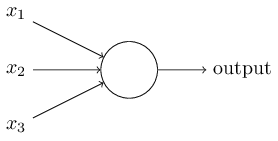
\includegraphics[scale=0.5]{img9.png}
    \caption{Exemple de la representation graphique d’un perceptron.}
\end{figure}

Dans ce cas le perceptron a 3 entrées, amis en général il peut avoir une quantité arbitraire d’entrées, Rosenbatt propose une règle simple pour calculer la sortie. En effet, il introduit de poids $w_1, w_2, ...$ qui représentent des nombres réels illustrant l’importance de chaque entrée respectivement avec la sortie. La sortie de la neurone ($0$ ou $1$)  résulte de la somme pondérée des entrées, si cette somme est supérieure à une valeur limite, la sortie sera égale à $1$, mais si elle est inferieurs à cette valeur limite la sortie sera $0$. 

%ecuacion
\begin{equation}
    output =
    \begin{cases*}
      0 & if $\Sigma_j w_jx_j \leq $ threshold \\
      1 & if $\Sigma_j w_jx_j > $ threshold \\
    \end{cases*}
\end{equation}

La valeur limite est aussi un nombre réel. Il s’agit d’un paramètre du neurone. Pr notation, on simplifie la description précédant en considérant $w$ et $x$ comme des vecteurs des poids et des entrées, respectivement, donc la somme pondérée devient : 

%ecuacion
\begin{equation}
    w \cdot x \equiv \Sigma_j w_jx_j
\end{equation}

Finalement, on définit le biais noté b comme $b \equiv -$threshold, alors on a: 

%ecuacion
\begin{equation}
    output =
    \begin{cases*}
      0 & if $w \cdot x + b \leq 0$ \\
      1 & if $w \cdot x + b > 0$ \\
    \end{cases*}
\end{equation}

Il faut comprendre le biais comme un objet de mesure qui permet de déterminé à quel point il est facile de faire que la sortie du perceptron soit égale à $1$. En termes biologiques, le biais est une mesure qui permet de savoir à quel point il est facile de faire que le perceptron se déclenche ou s’active. 

Même si les perceptrons sont très utilisés pour modéliser une grande variété de problèmes, ils ont un grand désavantage. En effet, un petit changement dans le vecteur des biais ou dans celui des poids, peut entrer un grand changent dans la sortie, ce qui peut être problématique, même dans le cas d’un algorithme de bas niveau d’apprentissage.
\hfill\\

\paragraph{Neurones Sigmoïdes}
Elles se représentent de la même façon que les perceptrons : 

%imagen
 \begin{figure}[H]
 \centering
    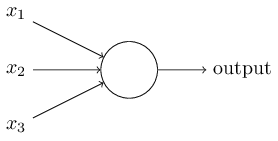
\includegraphics[scale=0.5]{img9.png}
    \caption{Exemple de la representation graphique d’une sigmoide.}
\end{figure}

Elles ont un nombre arbitraire d’entrées $x_1, x_2, ...$, mais les valeurs des entrées prennent de valeurs comprises entre 0 et 1. Elles possèdent aussi un poids pour chaque entrée, $w1, w2, ...$, et un biais $b$. Dans ce cas, les sorties ne sont pas de valeurs de $0$ ou $1$, mais une fonction $g(w\cdot x+b)$, où g est appelé la fonction sigmoïde ou en général, fonction d’activation, et est définie par : 

%ecuacion
\begin{equation}
    g(z)=\dfrac{1}{1+e^-z}
\end{equation}

Où $z=w\cdot x+b$. Graphiquement est définie par:

%imagen
 \begin{figure}[H]
 \centering
    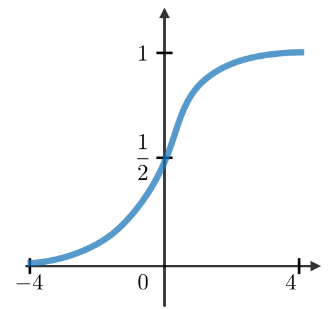
\includegraphics[scale=0.5]{img10.png}
\end{figure}

Dans ce cas, on observe que la sortie prend des valeurs entre $0$ et $1$, ceux qui revient à dire que la sortie peut prendre une infinité de valeurs. Usuellement, lorsqu’on emplois des sigmoïdes, l’intervalle est devisé en partitions et en fonction de la valeur obtenue, on fait une interprétation particulière de la sortie. Par exemple, en traitement d’image si on veut savoir si l’image d’entrée possède le numéro $9$, on pourrait employer une cote de $0.5$.  


\paragraph{Autres modèles de neurones utilisés dans le modèle}
La méthode RNNbruit emploie des réseaux de neurones avec de neurones sigmoïdes mais il peut employer deux autres modèles de neurones : $Tanh$ et $RELU$. Le comportement et la description de ces modèles est exactement le même, avec un changement de la fonction d’activation $g$. 

%imagen
 \begin{figure}[H]
 \centering
    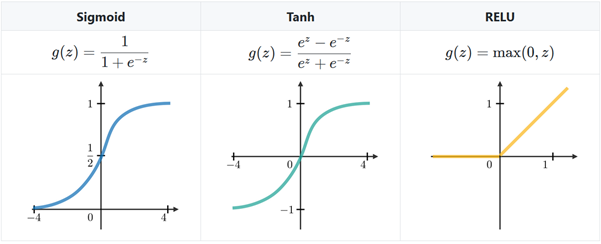
\includegraphics[scale=0.7]{img11.png}
\end{figure}


\subsubsection{Notation dans l’architecture des réseaux neuronales}
Les entrées sont encerclées et symbolisés : 

%imagen
 \begin{figure}[H]
 \centering
    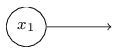
\includegraphics[scale=0.5]{img12.png}
\end{figure}

Considérons un réseaux neuronal arbitraire comme celui-ci-dessous : 

%imagen
 \begin{figure}[H]
 \centering
    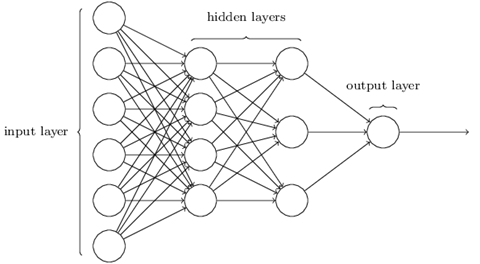
\includegraphics[scale=0.7]{img13.png}
\end{figure}


La colonne de gauche qui contient toutes les entrées est connue comme “couche d’entrée” (input layer en anglais). La colonne de droite qui contient toutes les sorties est connue comme “couche de sortie” (output layer en anglais). Les autres colonnes qui contiennent les neurones sont connues comme “couches cachés” (hidden layers en anglais). Dans le cas de l’image ci-dessus, on a un réseau neuronal avec 6 entrées (input features en anglais), 2 couches cachés et une sortie.  Il est important de remarquer que ce type de réseau neuronal, qui est composé d’une couche d’entrées, 2 couches cachées et une couche de sortie, est connue sous le nom de réseau neuronal pré-alimenté.
\hfill\\

\subsubsection{Réseau de neurones récurrents (Recurrent Neural Networks, RNN)}

Les réseaux de neurones récurrents sont un autre type de réseau de neurones. Il se caractérisent par le fait que la sortie donnée par une neurone est la sortie générale du réseau et au même temps, cette sortie est l’entrée pour le neurone suivante, comme l'illustre l'image ci-dessous : 

%imagen
 \begin{figure}[H]
 \centering
    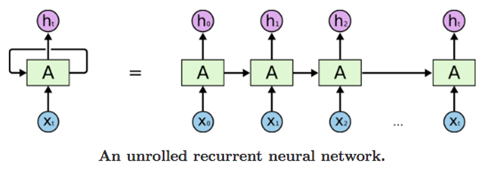
\includegraphics[scale=0.5]{img14.png}
\end{figure}


Le réseau de neurones récurrent est symbolisé comme le réseau de gauche avec une boucle de retro alimentation, cependant, il est plus de comprendre son fonctionnement en la “déroulant” (unroll en anglais) comme nous pouvons voire dans le réseau de neurones équivalent de droite. Dans ce cas, les neurones sont représentés par des rectangles en vert et la lettre $A$, les entrées sont représentées par des cercles bleus et la lettre $X$ avec un indice, et les sorties son représenté par des cercles violets et la lettre $h$ avec un indice. Il faut remarquer que dans ce cas la couche d’entrée correspond à la rangée qui contiens toutes les entrées en bleus, la couche de sortie correspond à la rangé supérieure qui contiens toutes les sorties en violet et la couche restante est la seule couche cachée. 

On observe que le neurone $A$, dans un premier temps, a comme entrée $X_0$. Elle réalise une fonction en fonction du type de neurone duquel elle fait partie et produit comme sortie la première sortie du réseau $h_0$.  Cette neurone fiat une retro alimentation avec la sortie qu’elle produit lorsque l’entrée est $X_1$ et ainsi de suite. Dans d’autres réseaux de neurones, les entrées sont indépendantes les unes avec les autres, mais dans le cas des réseaux de neurones récurrents toutes les entrées sont reliées avec les autres. 

C’est-à-dire qu'un réseau de neurones récurrents, contrairement à un réseau de neurones pré alimenté, peut utiliser l’état internet des neurones (mémoire) pour traiter des séquences d’entrées. Ceci explique pourquoi elles peuvent être utiliser pour des travaux comme la reconnaissance d’écriture ou vocale. 

La formule qui décret la sortie d’un réseau de neurones récurrent est la suivante :

\begin{equation}
    h_t = g(w_{t-1}h_{t-1} + w_tX_t) 
\end{equation}


Où g est la fonction d’activation du neurone.  

\subsubsection{\textbf{RNNbruit: Méthode hybride DSP/Deep Learning}}
\medskip
\hfill
\medskip
Après avoir compris les concepts précédents, il est beaucoup plus facile de comprendre la méthode et comment elle fonctionne. Dans un premier temps, \textbf{l’atténuation du bruit} est un sujet qui a toujours causé problème dans le traitement de la voix (\textbf{speech processing}), \href{https://ieeexplore.ieee.org/document/1163209} (qui date des années 70), et comme son nom l’indique, l’idée est simple : il suffit de prendre un signal bruité et éliminer le plus grand nombre de bruit possible sans causer de pertes d’information ou de distorsion pour l’audio qui nous intéresse. 
%imagen
 \begin{figure}[H]
 \centering
    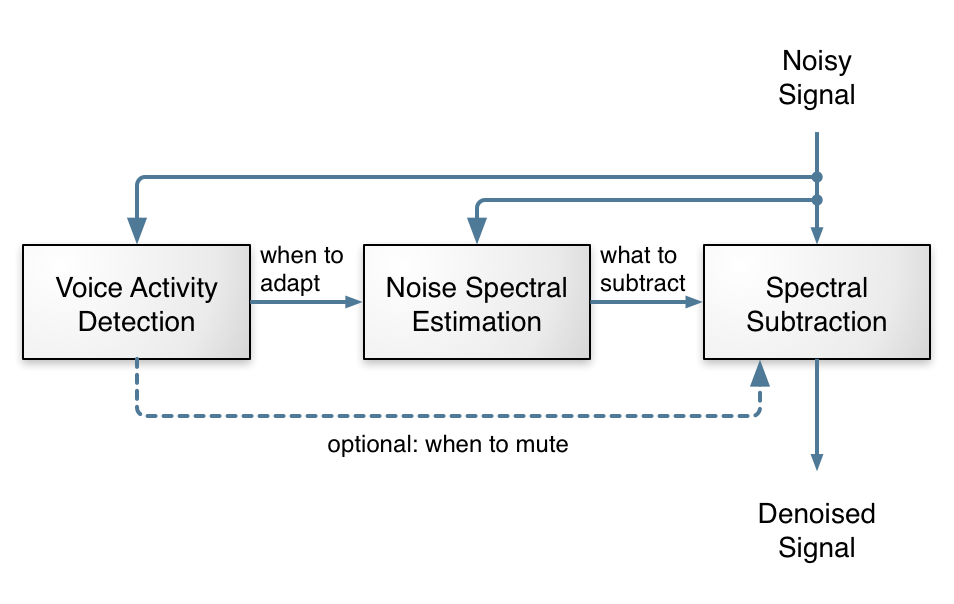
\includegraphics[scale=0.7]{noise_suppression.png}
    \caption{Ceci est la vision conceptuelle d’un algorithme conventionnel d’atténuation du bruit. Un modèle de détection de l’activité de la voix ou VAD (\textit{Voice Activity Detection}) détecte le signal qui contient la voix et le bruit. Ceci est utilisé par un modèle d’estimation spectral du bruit (\textit{Noise Spectral Estimation}) pour déchiffrer les caractéristiques spectrales du bruit. Ensuite, sachant comment est bruit, celui-ci peut être « soustrait » (ce n’est pas aussi facile que ça semble) de l’audio qui est l’entrée du modèle }
    \label{Figure 14}
\end{figure}
Le seul problème de l’image ci-dessus est qu’il semblera que la suppression du bruit est simple : Faire ces 3 taches conceptuel et c’est fini. Ceci n’est pas tout à fait vrai, car \underline{le plus difficile} est de faire que l’algorithme soit configuré minutieusement et attentivement pour chaque cas particulier. Par conséquent, l’opinion la plus courante sur ce sujet se résume en « 50\% science, 50\% art ».
Après avoir compris cela, il est temps d’explique et comprendre le \textbf{deep learning et les réseaux de neurones récurrents}. Le deep learning est une nouvelle version d’une idée ancienne : réseau de neurones artificielles. Bien que ce soit derniers sont utilisée depuis les années 60, ce qui est nouveau est :

\begin{enumerate}
    \item Maintenant on sait comment faire plus de 2 couches cachés
    \item On sait comment faire que les réseaux récurrents des patrons du passé
    \item On a des ressources de calcul pour les trouvés
\end{enumerate}

Les réseaux de neurones récurrents sont très importants pour cette méthode parce qu’elles modèlent de séquences de temps au lieu de considéré uniquement les entrées et les sorties indépendamment. Ceci est important pour l’atténuation ou élimination du bruit \underline{car on a besoin du temps pour obtenir une bonne estimation du bruit}. Durant un certain temp les RRNs étaient  hautement limité dans son activité à cause de deux problèmes : elles ne pouvaient pas retenir l’information pendant un long période de temps et parce que le processus de l’algorithme du gradient impliqué dans la rétropropagation du gradient \textit{backpropagating} au cours du temps était inefficace (il s’agissait d’un problème d’évanouissement du gradient). Ces deux problèmes ont été résolu avec l’invention des \textit{unités fermées} (\textit{gated units}), comme les LSTM (\textit{ Long Short-Term Memory}), les GRU (\textit{Gated Recurrent Unit}), entre autres.

RNNbruit utilise les unités récurrentes fermées (GRU) parce que celles-ci ont un meilleur fonctionnement que les LSTM pour cette tâche et demandent moins de ressources de calcul (CPU et mémoire). En comparant les avec les unités récurrentes simples, les GRU ont deux portes supplémentaires. La porte de redémarrage (\textit{reset gate}) vérifie si l’état (mémoire) est utilisé dans le calcul du nouvel état, alors que la porte de mise à jour (\textit{update gate}) contrôle combien va changer l’état basé sur la nouvelle entrée. Grace a la  porte de mise à jour (lorsqu’elle est éteinte) le GRU a le pouvoir de se rappeler de l’information pendant une période de temps plus longue et est la raison porque laquelle les Gru (et le LSTM) exécutent d’une meilleur façon les unités récurrentes simples.

%imagen
 \begin{figure}[H]
 \centering
    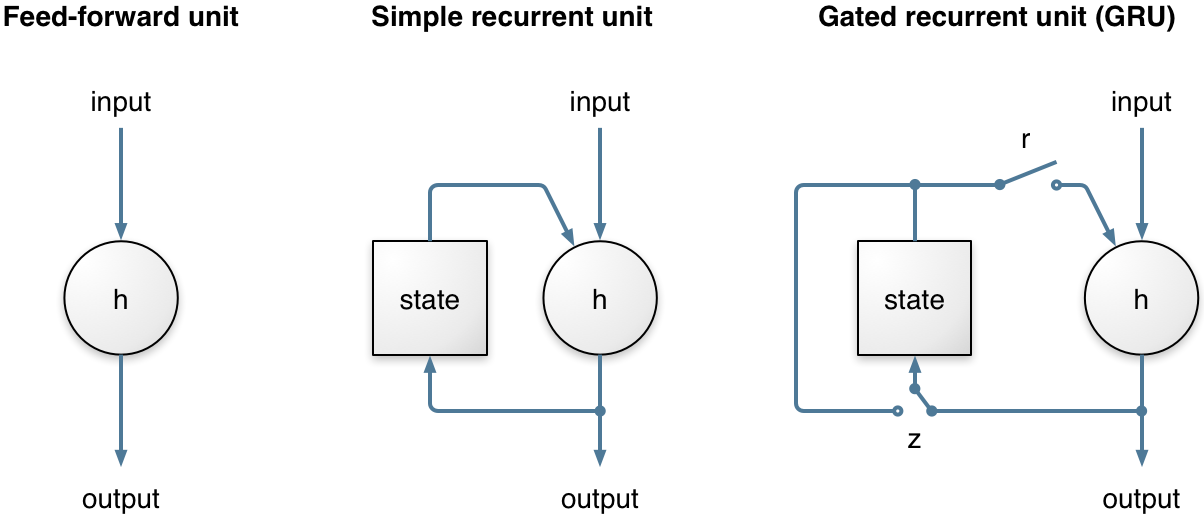
\includegraphics[scale=0.7]{simple_vs_gru.png}
    \caption{Comparaison d’une unité simple récurrente avec un GRU. La différence se trouve sur les portes $r$ er $z$ de la GRU, qui rendent possible l’apprentissage des patrons a long therme. Toutes les deux sont des interrupteurs doux (\textit{soft switches} avec de valeurs comprises entre 0 et 1) calculés sur l’état antérieur de tout la couche et les entrées, avec une fonction d’activation sigmoïde. Lorsque la porte de mise à jour $z$ est à gauche, alors l’état peut rester constant sur une longue période de temps $-$ jusqu’à  qu’une condition entraine que la porte $z$ change vers la droite.} 
\end{figure}
Grace au succès du deep learning, il est, maintenant, populaire de « tirer » des réseaux de neurones deep a un problème complet. Ces approches sont connues sous le nom de \textit{end-to-end} $-$ où il s’agit de neurones du début à la fin. De plus, ils ont été appliqués au \href{https://arxiv.org/pdf/1412.5567.pdf}{reconnaissance de la voix \textit{(speech recognition)}} et au \href{https://deepmind.com/blog/article/wavenet-generative-model-raw-audio}{synthese de la voix (\textit{speech synthesis})}. D’une part, ces systèmes \textit{end-to-end} optimales, tanto anti-productif en termes de ressources. Par exemple, certaines approches d’atténuation  ou d’élimination du bruit utilisent des milliers de neurones et de décennies de millions des poids  (\textit{weights}) pour réaliser l’atténuation. Il ne s’agit pas uniquement d’un problème de cout de calcul, mais aussi de taille propre du modèle, où il y a des milliers de lignes de code et de décennies de mégabytes (ou plus) de poids de neurones.  

Pour cette raison, la méthode de RNNbruit utilise une \textit{approche hybride} : maintenir tout le processus basique du traitement de signal (empêche que le réseau de neurones essaye de l’émuler) mais laisser que le réseau de neurones apprenne toutes les parties compliquées qui demandent d’une configuration sans fin en parallèle au processus du traitement du signal.

%imagen
 \begin{figure}[H]
 \centering
    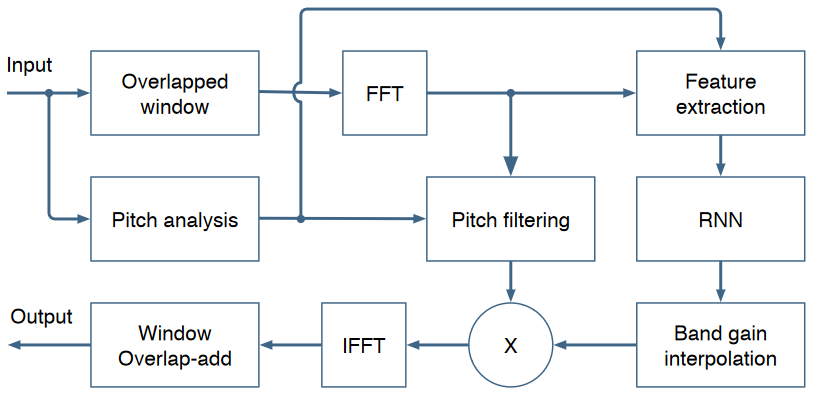
\includegraphics[scale=0.7]{Block_Diagram.png}
    \caption{Diagramme de blocs, où le réseau de neurones est représenté par le bloque RNN et toute l’approche deep correspond à la colonne de droite, le reste fait partie du processus du traitement du signal. Ceci met en évidence l’approche hybride qui travaille en parallèle.}
    \label{Figure 16}
\end{figure}

Un autre aspect diffère à certains des travaux existant sur l’atténuation du bruit avec le deep learning est qu’il vise une communication en temps réel au lieu d’une reconnaissance de la voix. Par conséquent, il ne peut pas regarder vers l’avant pas plus de quelques millisecondes (dans ce cas $10 ms$).
\medskip

\paragraph{\textbf{Définition du problème}}
\hfill\\
\hfill
Pour éviter la création d’un grand nombre de sortir $-$ et par conséquent, un grand nombre de neurones $-$ la méthode a été créé pour quelle ne travaille pas directement avec des échantillons (\textit{samples}) ou un spectre. Au contraire, elle considère des \textit{groupes} (\textit{bands}) de fréquences qui suivent l’échelle de Bark. Une échelle de fréquences qui coïncide avec la façon dont nous percevons les sons. Arrivant, ainsi, a utilisé un total de 22 groupes, au lieu de 428 valeurs spectrales (complexes) qui aurait dû être considéré.

%imagen
 \begin{figure}[H]
 \centering
    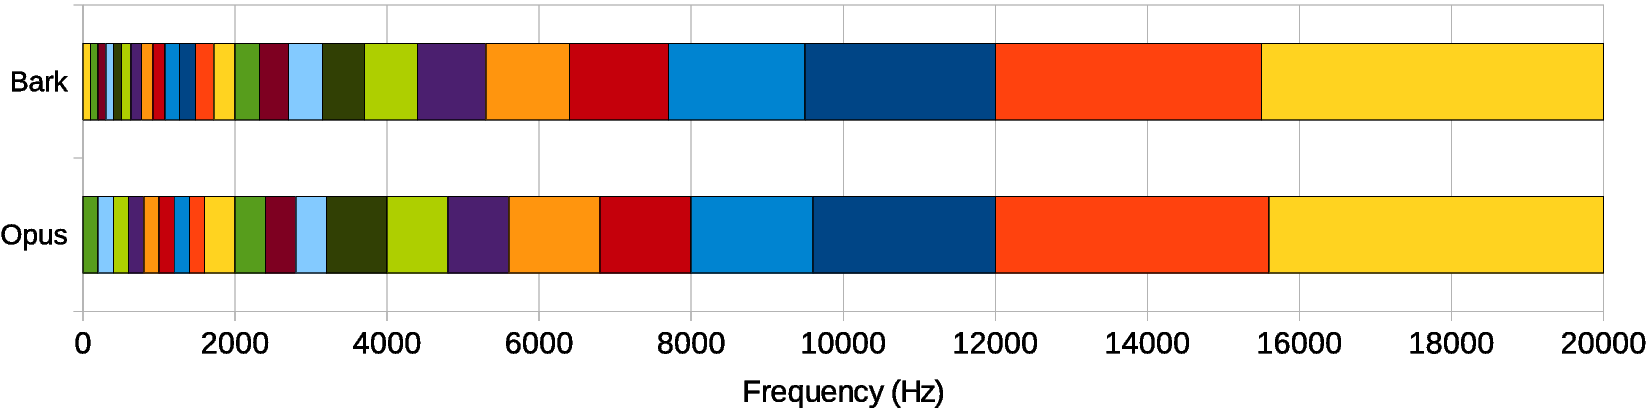
\includegraphics[scale=0.25]{bands.png}
    \caption{Comparaison de groupes Opus et l’échelle de Bark. Pour RNN bruit, on utilise Opus comme base. Etant donné qu’on superpose les groupes, les limites sont que les groupes d’Opus se transforment au centre des groupes superposé de RNNbruit. Les groupes sont plus larges à haute fréquence parce qu’ouïe a une petite résolution de fréquence pour ces hautes fréquences. A bases fréquences, les groupes sont plus étroites, mais pas aussi larges comme celles de l’échelle de Brak parce que dans ce cas, on n’aurait pas accès de donné pour faire des estimations.} 
\end{figure}
Il est clair qu’on ne peut pas reconstruire un audio avec seulement 22 groupes d’énergies. Mais ce qu’on peut faire est calculer un gain qu’il faut applique au signal pour chacun de ses groupes. Une manière simple de l’imaginer est de pensé a utilisé un égaliseur de 22 groupes et rapidement changer le niveau ou le volume pour chaque groupe pour atténuer le bruit mais laisser passer le signal. 

%imagen
 \begin{figure}[H]
 \centering
    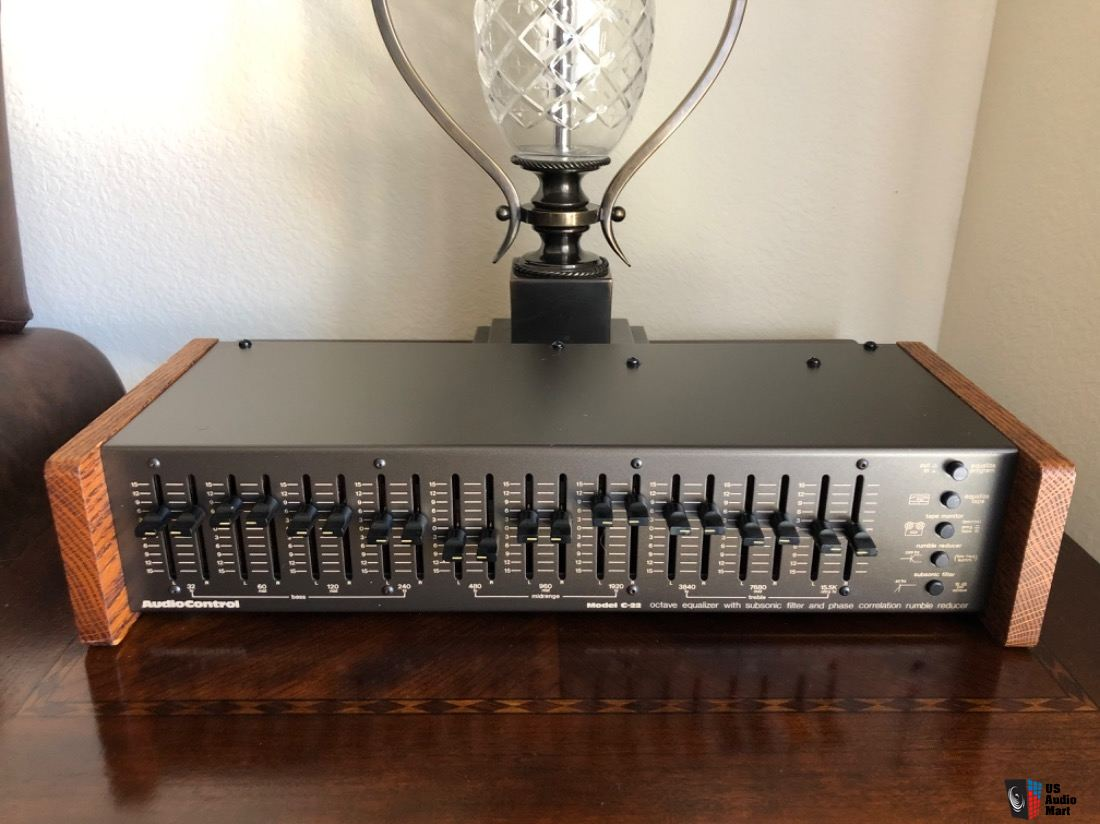
\includegraphics[scale=0.2]{22bEq.jpg}
    \caption{Egaliseur graphique vintage \href{https://www.canuckaudiomart.com/details/649586296-vintage-audio-control-c-22-octave-10-band-equalizer/images/2554905/}{AudioControl C-22}.Chacun des butons verticaux qui montent et descendent (\textit{faders}) représentent le volumen d’une fréquence en particulier; RNNbruit fonctionne de façon similaire.} 
\end{figure}
Il y a plusieurs avantages de travailler avec des gains par groupe :
\begin{enumerate}
    \item On obtient un modèle plus simple parce qu’on calcul moins de groupes
 \item Il est impossible de créer les  \href{https://www.vocal.com/noise-reduction/musical-noise/}{"artefacts de bruit musical" (\textit{musical noise artifacts})}, où uniquement un ton arrive a passé alors que ses « voisins » sont atténués. Ces artefacts sont communs dans l’atténuation du bruit et sont très embêtants. Avec des groupes suffisamment larges, on laisse passer tout le groupe complet ou on le coupe en entier.
    \item L’optimisation du modèle. Comme les gains de groupes sont toujours organisé entre $0$ et $1$. Il suffit d’utiliser une fonction d’activation sigmoïde (dont la sortie est entre $0$ et $1$) pour les calculer. Ça garantie qu’on ne peut jamais faire quelque chose de stupide, comme ajouter du bruit qui n’était pas présent.  
\end{enumerate}
Le désavantage principal de la mineur résolution, qu’on obtient en utilisant les groupes, est qu’on n’a pas une résolution suffisamment fine pour atténuer le bruit entre les harmoniques du ton (\textit{pitch harmonics}). Heureusement, ceci n’est pas très important et on peut le réaliser avec un signal basique comme on peut voir dans le modèle \textit{Pitch filtering} sur la \ref{Figure 16}.

\medskip
\paragraph{\textbf{Architecture deep}}
\hfill\\
Comme la sortie est calculé sur 22 groupes, il n’y a pas de sens d’avoir une plus grande fréquence de résolution de l’entrée. Alors on utilise les mêmes 22 groupes pour éviter d’envoyer l’information spectral au réseau de neurones. Du fait que \href{https://www.britannica.com/science/dynamic-range}{l’audio un grand rand dynamique}, il est préférable de calculer le $logarithme$ de l’énergie au lieu d’envoyer l’énergie directement. On utilise un processus de décorrélation (\textit{decorrelate}) des caractéristiques en utilisant une \href{https://dsp.stackexchange.com/questions/27810/how-to-understand-the-de-correlation-property-of-dct-what-does-de-correlation-m}{tranformée discrète du cosinus (DCT, \textit{Discrete Cosine Transform})}. Résultant dans une \href{https://es.wikipedia.org/wiki/Cepstrum}{\textit{cepstrum}} basé sur l’échelle de Bark, lequel est très lié avec les Coefficiente Cepstrales de fréquence-Mel (MFCC, \href{https://en.wikipedia.org/wiki/Mel-frequency_cepstrum}{\textit{Mel-Frequency Cepstral Coefficients})}qui sont habituellement utilisé dans la reconnaissance de la voix.

En addition au coefficients, RNNbruit comprend également :

\begin{itemize}
    \item La première et la deuxième dérivée de 6 premiers coefficients  \textbf{(12 caractéristiques de l’entrée)}
    \item La période du ton ($1$/\textit{fréquence fondamental}) \textbf{(1 caractéristique de l’entrée)}
    \item Le gain du ton  (\textit{voicing strength}) en 6 groupes \textbf{(6 caractéristiques de l’entrée)}
    \item Une valeur spéciale pour la détection de la \textbf{(1 caractéristique de l’entrée)}
\end{itemize}

\hfill\\
Ce qui veut dire que RNNbruit utilise au total 42 caractéristiques de l’entrée au réseau de neurones récurrent, on peut voir cela dans l’image ci-dessous


%imagen
 \begin{figure}[H]
 \centering
    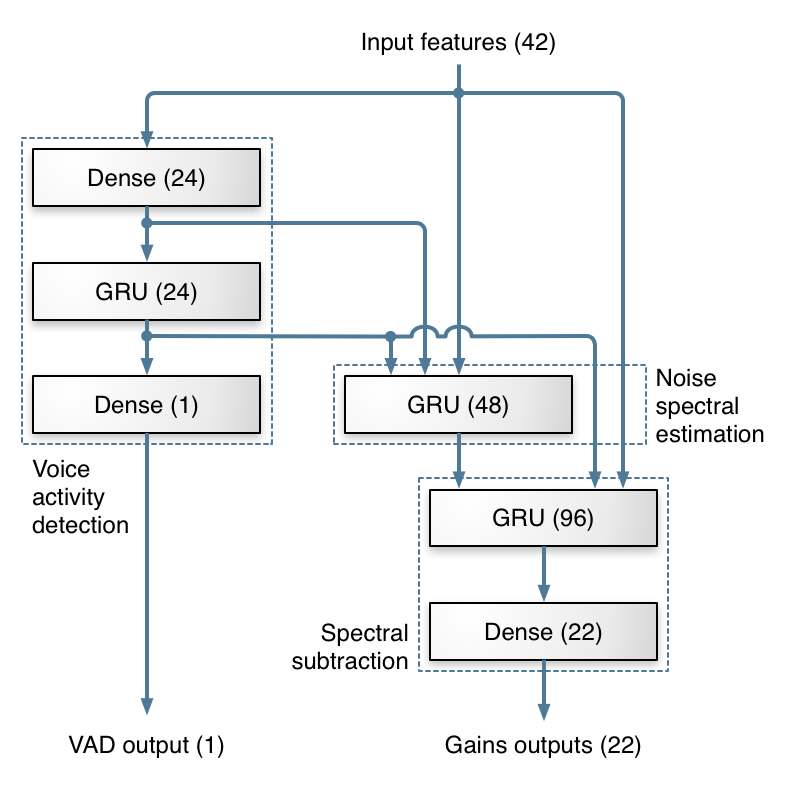
\includegraphics[scale=0.7]{topology.png}
    \caption{Topologie d’un réseau de neurones qui utilise RNNbruit. Chaque boite représente une couche de neurones, avec le numéro d’unités indiqué entre parenthèses. Les couches denses (\textit{Dense}) sont des couches non récurrentes, cependant les GRU sont clairement récurrentes. Une des sorties du réseau est un ensemble de gain qu’il faut appliquer aux 22 groupes de fréquences  (\textit{Gains outputs (22)}). L’autre sortie est probabilité d’activation  \textit{VAD output(1)}), quo n’est pas utilisé dans le processus d’atténuation du bruit mais qui est un sous-produit du.} 
\end{figure}
L’architecture deed utilisé s’inspire dans l’approche traditionnel de l’atténuation du bruit comme on peut voir dans la \ref{Figure 14}. Il faut remarquer que dans ce cas, chacun des 3 modules utilise des réseaux de neurones et ils se trouvent encadré par des lignes pointillées bleus. La plupart du travail est réalisé par les 3 couches de GRU. Aussi, il faut remarquer que dans le cas des réseaux de neurones, il n’y a pas de preuves qu’on utilise les couches de la façon qu’on prétend, mais le fait que la topologie fonctionne d’une meilleure façon que pour les autres qui ont été essayé par les créateurs de la méthode, fait que ça soit raisonnable de penser qu’elle se comporte de la façon qu’elle a été créer. 

\paragraph{\textbf{Code et implémentation}}
Le code de la méthode est de libre accès et est disponible sur le répertoire de GitHub \href{https://github.com/xiph/rnnoise}{xiph/rnnoise}.Tout le desing et l’entrainement du réseau de neurones est écrit en Python en utilisant la librairie propre au deep learning \href{https://keras.io/}{Keras}, mais tout le code d’exécution est écrit en C sous une \href{https://es.wikipedia.org/wiki/Licencia_BSD}{licencia BSD} un type de système d’exploitation type Unix.
Le système d’exploitation choisi pour ce travail est \href{https://ubuntu.com/download/desktop}{Ubuntu 20.04.1} un système d’exploitation (64-bit) open source. Cependant, du fait que ce système d’exploitation n’est pas le système d’exploitation de préférence personnelle, on a décidé d’utiliser une machine virtuelle en employant le software \href{https://www.virtualbox.org/}{Oracle VirtualBox 6.1} (une autre software open source), en utilisant comme système d’exploitation principal ou \textit{host} Microsoft Windows 10 Home Single Language. Sur l’image ci-dessous, on peut voir la machine virtuelle choisit, ainsi que les caractéristiques choisies. Il faut remarque qu’entre les caractéristiques on peut voir qu’il y a un dossier partager entre le \textit{host} et la machine virtuelle. Ceci est pour rendre plus facile l’entrée et la sortie des fichiers par la méthode.

%imagen
 \begin{figure}[H]
 \centering
    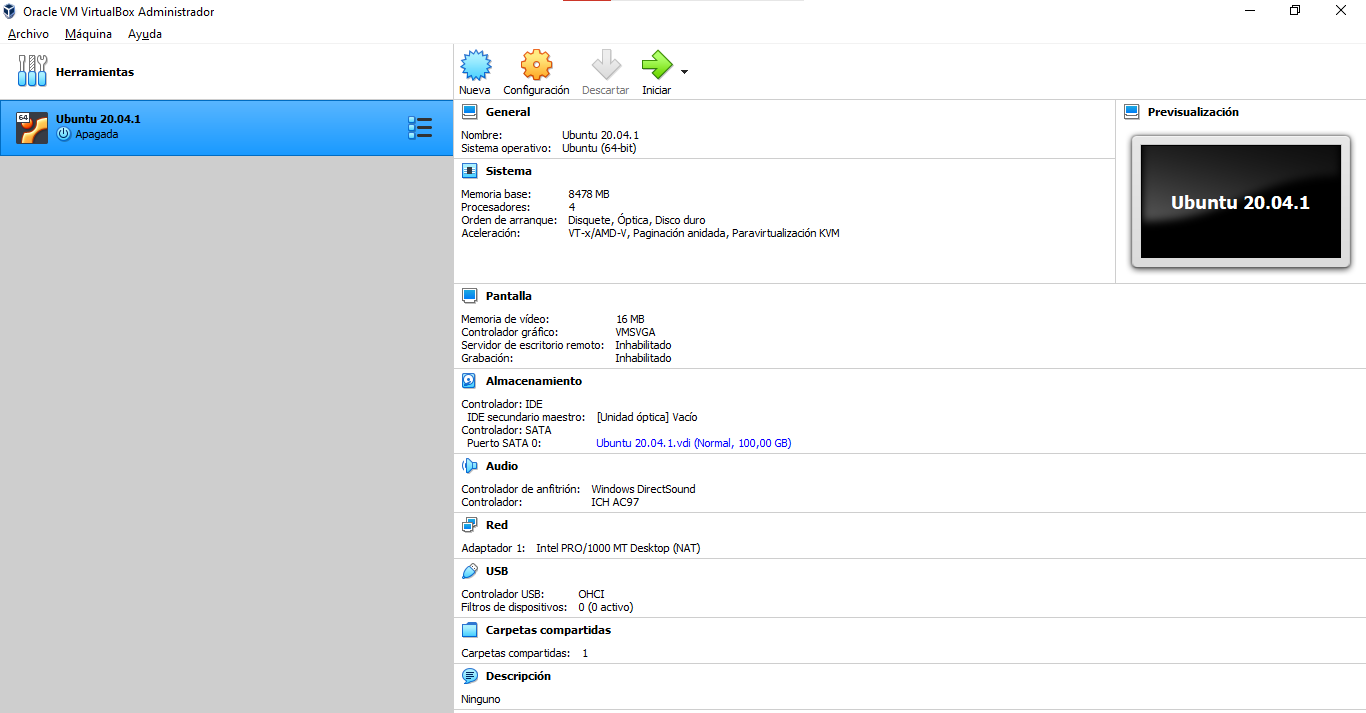
\includegraphics[scale=0.45]{VM1.png}
    \caption{ Caractéristiques de la machine virtuelle de Ubuntu implémenté} 
\end{figure}

Ci-dessous, on peut voir une capture d’écran du fonctionnement de la machine virtuelle.

%imagen
 \begin{figure}[H]
 \centering
    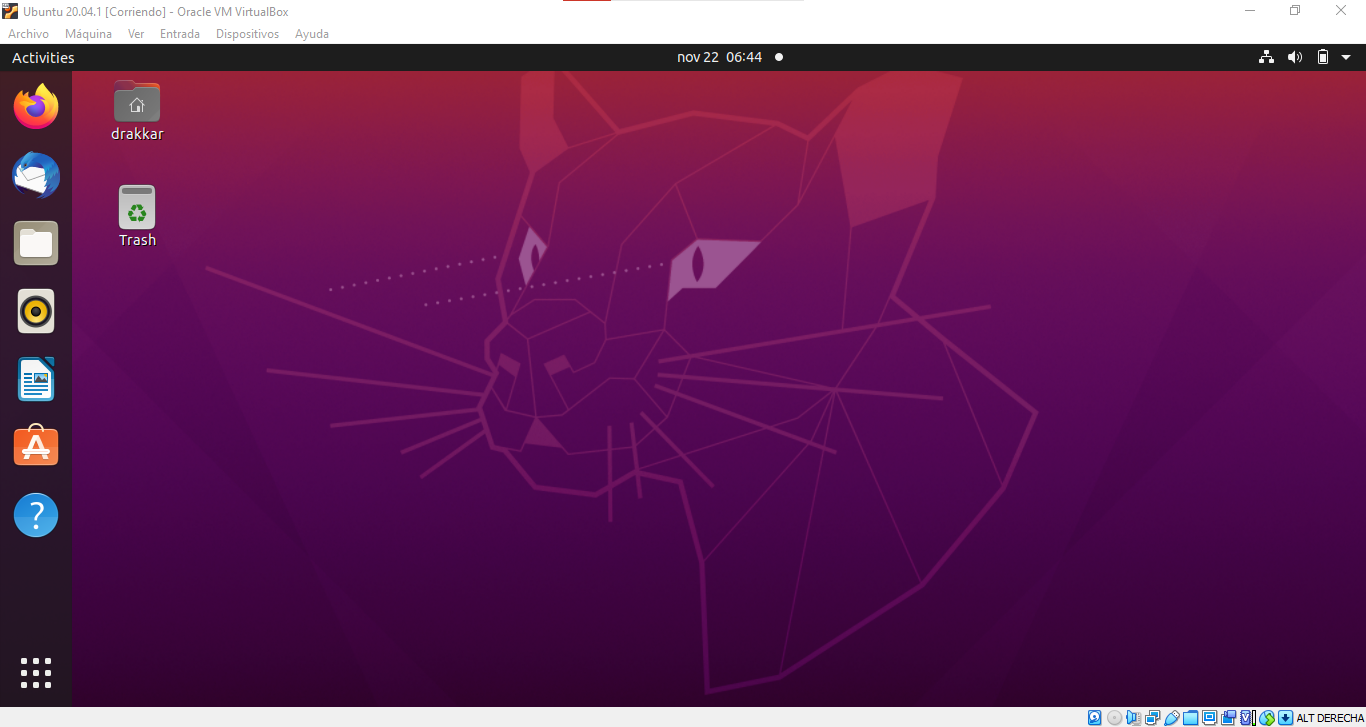
\includegraphics[scale=0.45]{VM2.png}
    \caption{Machine virtuelle allumé} 
\end{figure}
\hfill\\
Après avoir téléchargé le code du repositoire GitHub précèdent, on a suivi les instructions du \texttt{README} disponible sur le répertoire, afin fin « d’activer » la méthode. Les instructions se trouvent ci-dessous.

%imagen
 \begin{figure}[H]
 \centering
    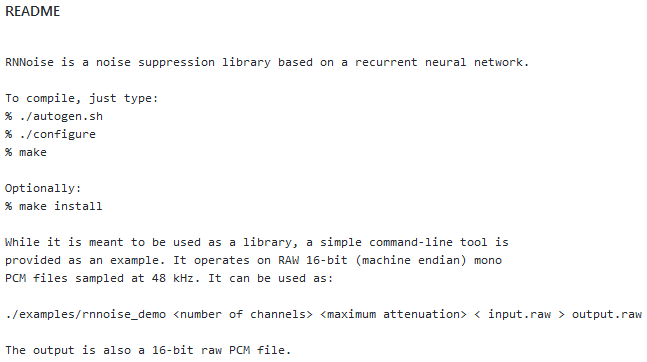
\includegraphics[scale=0.7]{VM3.png}
    \caption{Instructions pour activer ou compiler la méthode de RNNbruit} 
\end{figure}

En suivant les instructions, on peut voir un exemple de l’exécution de la méthode RNNbruit en utilisant comme exemple l’audio en entrée \texttt{AW0,3.wav} et en spécifiant le nombre de l’audio de sortie \texttt{SALIDA.wav}.

%imagen
 \begin{figure}[H]
 \centering
    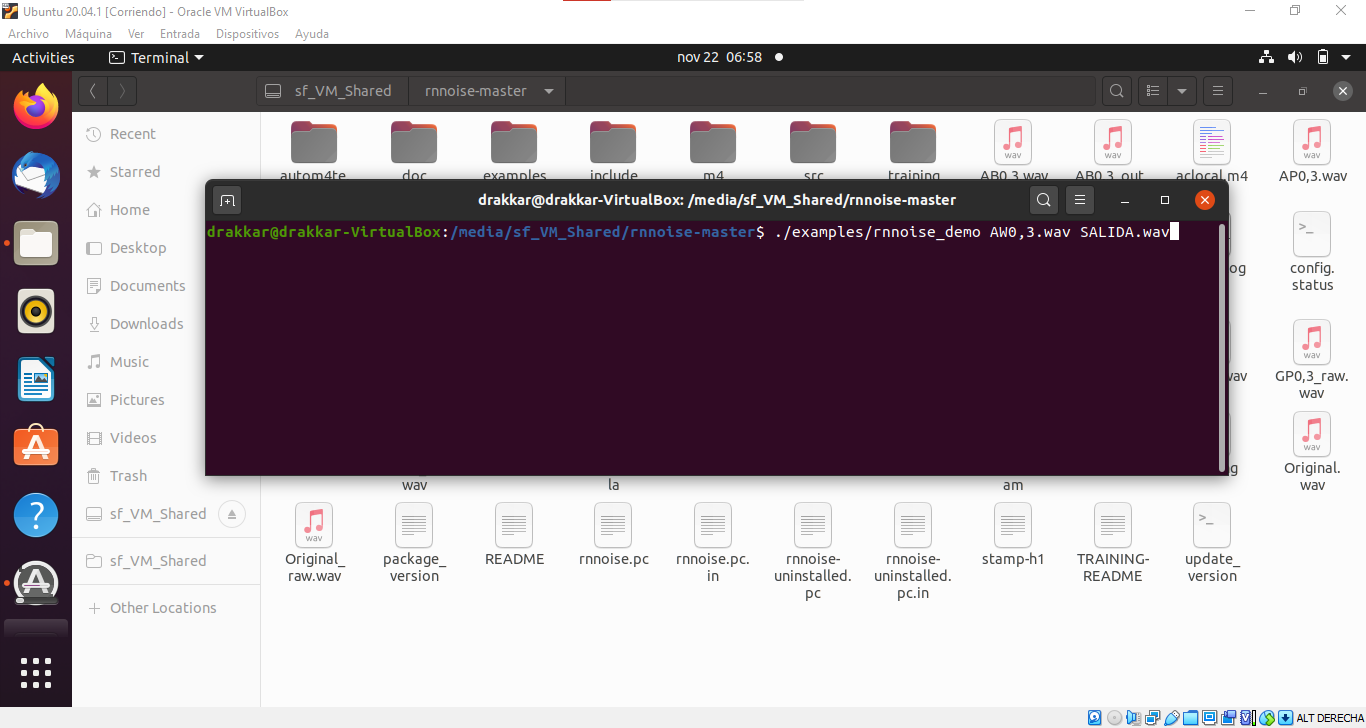
\includegraphics[scale=0.45]{VM4.png}
    \caption{Exécution de la méthode RNNbruit } 
\end{figure}
\hfill\\

On observe sur l’image ci-dessous que l’exécution de la méthode s’est réalisée avec succès et le fichier \texttt{SALIDA.wav} a été créé.
%imagen
 \begin{figure}[H]
 \centering
    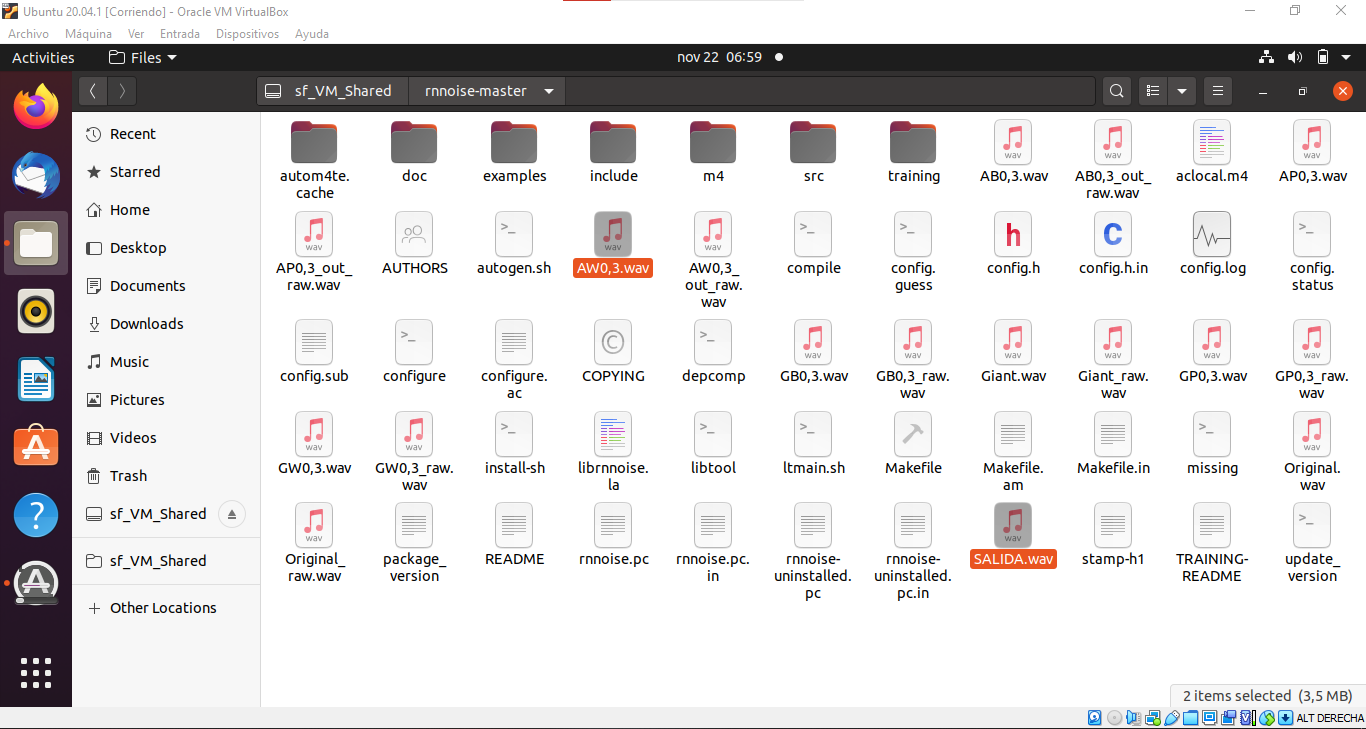
\includegraphics[scale=0.4]{VM5.png}
    \caption{Audio en entrée et audio résultant en sortie} 
\end{figure}

Même si l’audio résultant est enregistré sous forma \texttt{.wav}, les instructions de la méthode disent qu’en réalité ils sont enregistrés dans un fichier du typo \texttt{RAW PCM 16-bit}. Par conséquent, si on essaye de l’ouvrir ou de le reproduire, il se produit une erreur. On peut voir ce comportement sur l’image ci-dessous. 

%imagen
 \begin{figure}[H]
 \centering
    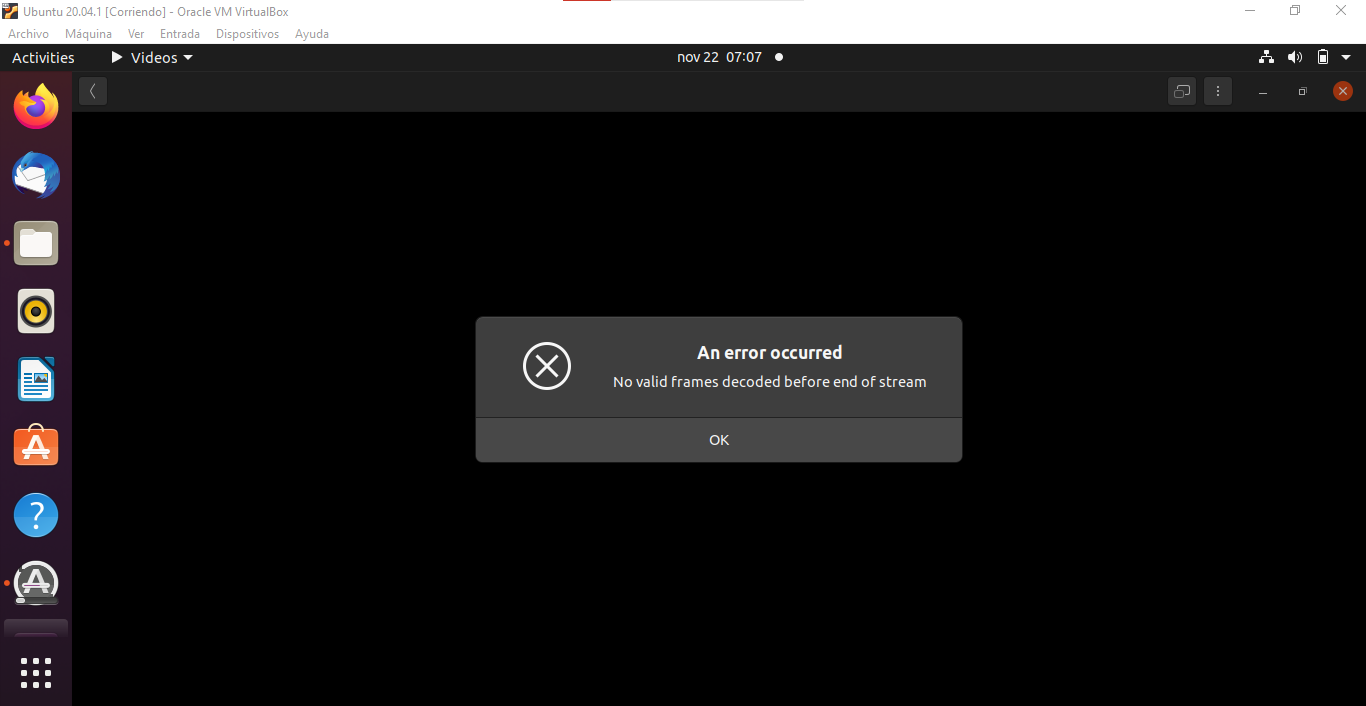
\includegraphics[scale=0.4]{VM6.png}
    \caption{Erreur obtenu lorsqu’on essaye de reproduire l’audio résultant} 
\end{figure}

Pour corriger ce format de l’audio en sorte, on revient sur le système d’exploitation \textit{host}, on utilise le software open source \href{https://www.audacityteam.org/}{Audacity 2.4.2} et on prend le fichier du dossier partager avec la machine virtuelle. Pour l’ouvrir de la bonne façon sur Audacity, on utiliser les options \texttt{File/import/Raw Data...} comme on peut le voir dans l’image ci-dessous. 

%imagen
 \begin{figure}[H]
 \centering
    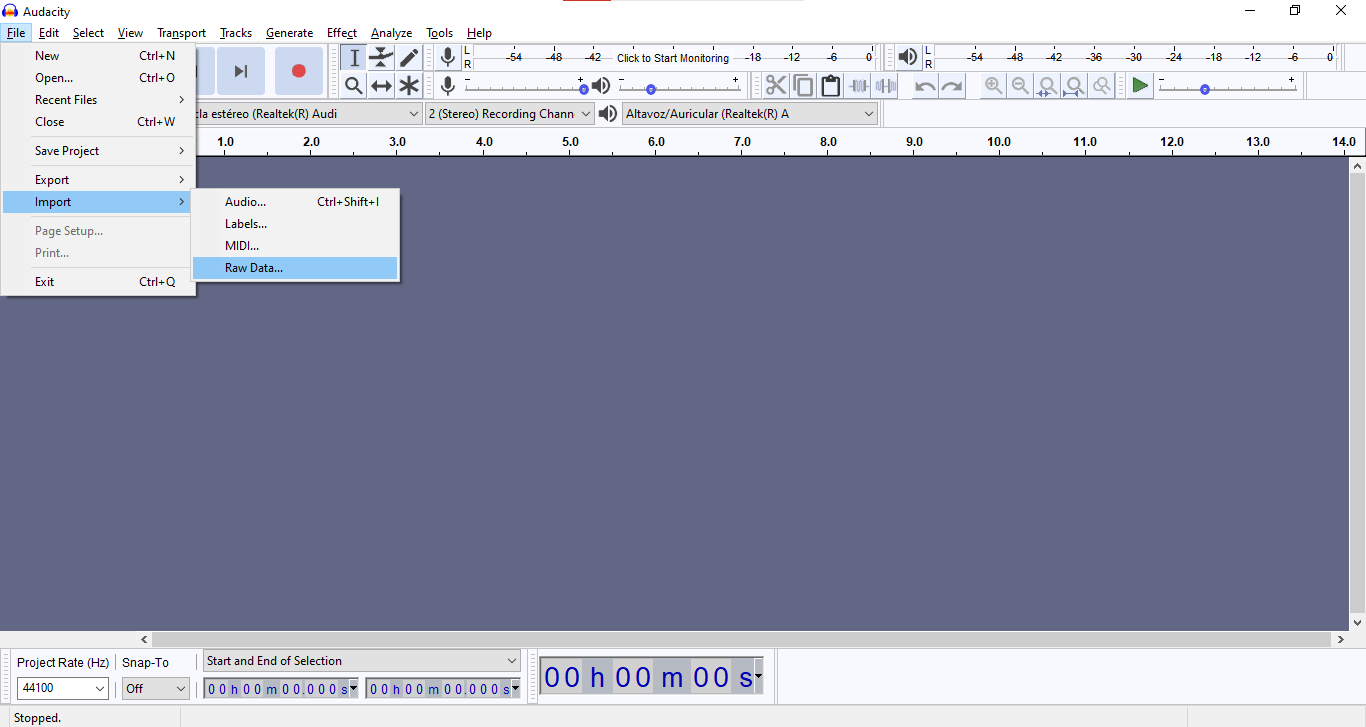
\includegraphics[scale=0.4]{VM7.png}
    \caption{Importation de l’audio de sortie sur Audacity}
\end{figure}
On sélectionne le fichier du dossier partager.

%imagen
 \begin{figure}[H]
 \centering
    \includegraphics[scale=0.45]{VM8.png}
\end{figure}
Et on l’importe avec les respectives configurations. 
%imagen
 \begin{figure}[H]
 \centering
    \includegraphics[scale=0.6]{VM9.png}
\end{figure}

En important avec succès l’audio de façon qu’il soit reproductible sur Audacity.

%imagen
 \begin{figure}[H]
 \centering
    \includegraphics[scale=0.4]{VM10.png}
\end{figure}

Lequel peut être exporter avec succès tout simplement en suivant les options \texttt{File/Export/Export as WAV} comme on peut voir sur l’image ci-dessous. 
.
%imagen
 \begin{figure}[H]
 \centering
    \includegraphics[scale=0.4]{VM11.png}
\end{figure}

En générant de manière satisfaisante l’audio de sortie en format reproductible.
%imagen
 \begin{figure}[H]
 \centering
    \includegraphics[scale=0.5]{VM12.png}
\end{figure}


\newpage
\section{Résultats et comparaison des méthodes}
Les méthodes ont été implémenter de manière qualitative et quantitative. Pour chaque cas, on a utilisé le software Matlab R2020a sur le SO Microsoft Windows 10 Home Single Language (v.10.0.19041). Pour les cas de l’implémentation a génère du bruit blanc, du bruit rose et du bruit rouge en utilisant le software Audicity 2.4.2. Après, sur Matlab on a pris l’enregistrement audio original et on a créé, à partir de ce dernier, 3 autres enregistrements audios en ajoutant 30\% du bruit blanc, 30\% du bruit rose et 30\% du bruit rouge, respectivement.

\subsection{Résultats quantitatifs}
Dans le tableau \ref{table:t1} on peut voir le pourcentage de bruit résultant lorsqu’on ajoute 30\% de bruit blanc a l’enregistrement audio et on le filtre avec chaque méthode.
\begin{table}[H]
    \centering
    \begin{tabular}{ l  c }
    \textbf{Méthodes} & \textbf{Blanc (30\%)} \\
    \hline
    Sans méthode & 80.658 \\
    Wiener & 44.218 \\
    Butter T & 10 \\
    RNNbruit & 9.9668 \\
    \end{tabular}
    \caption{Résultats des méthodes pour 30\% du bruit Blanc}
    \label{table:t1}
\end{table}
\hfill \\
Dans le tableau \ref{table:t2} on peut voir le pourcentage de bruit résultant lorsqu’on ajoute 30\% de bruit rose a l’enregistrement audio et on le filtre avec chaque méthode.
\begin{table}[H]
    \centering
    \begin{tabular}{ l  c }
    \textbf{Méthodes} & \textbf{Rose (30\%)} \\
    \hline
    Sans méthode & 39.442 \\
    Wiener & 44.082 \\
    Butter T & 35 \\
    RNNbruit & 11.493 \\
    \end{tabular}
    \caption{Résultats des méthodes pour 30\% du bruit Rose}
    \label{table:t2}
\end{table}
\hfill \\
Dans le tableau \ref{table:t3} on peut voir le pourcentage de bruit résultant lorsqu’on ajoute 30\% de bruit rouge a l’enregistrement audio et on le filtre avec chaque méthode.
\begin{table}[H]
    \centering
    \begin{tabular}{ l  c }
    \textbf{Méthodes} & \textbf{Marron (30\%)} \\
    \hline
    Sans méthode & 53.969 \\
    Wiener & 36.209 \\
    Butter T & 35 \\
    RNNbruit & 7.7496 \\
    \end{tabular}
    \caption{Résultats des méthodes pour 30\% du bruit Marron}
    \label{table:t3}
\end{table}
\hfill \\

Premièrement, en étudiant les résultats obtenus par l'implémentation du filtre passe-bas avec une approximation de Butter Worth, nous confirmant les hypothèses théoriques vues précédemment. En effet, compte tenu que l’approximation de Butter Worth permet d’avoir une précision en amplitude. Cette précision est centre sur des bases fréquences. Nous voyons cela évidence dans le filtrage des bruits ajouter à notre signal. Lorsque nous ajoutons du bruit blanc et nous filtrons le signal résultant, nous constatons une diminution du pourcentage du bruit présent dans le signal. Alors que lorsque nous effectuons le même procédé pour le bruit rose et le bruit marron, le pourcentage de bruit ne change pas. Donc cette méthode avec cette approximation particulière est bien plus convenable pour filtrer le bruit blanc présent dans les enregistrements audios.

Dans un deuxième temps, le cas de la méthode hybride du RNNbruit, nous observons que cette méthode est belle et bien convenable pour les différents types de bruit additionnés. En effet, nous constatons une atténuation du bruit considérable dans chacun des cas. De plus, nous remarquons que cette méthode ne gêne pas la transmission du signal sonore, en d'autre thermes cette méthode lise et "purifie" le signal orignal. Nous pouvons expliquer ce comportement par la nature adaptative de la méthode, dû au fait de l'implémentation de réseau de neurones récurrents pour faire face au bruit non harmonique. Cependant, la partie traditionnelle de cette méthode dite hybride se charge du bruit harmonique comme nous l'avant vue précédemment dans la partie théorique.

Finalement, lorsque nous analysons les résultats obtenus en utilisant le filtre adaptatif de Weiner, nous apercevons que cette méthode de filtrage numérique a des meilleurs résultats sur du bruit blanc. Or, en effectuant une analyse auditive, nous pourrions penser que ce filtrage est bien plus efficace avec le bruit marron ou le bruit rose, nous pouvions affirmer théoriquement que ‘est avec le bruit blanc qu’il est plus efficace. En effet, en employant cette méthode nous introduisons des nouveaux types de bruits que nous ne considérerons pas dans notre analyse. Par exemple, dans le filtrage de l’enregistrement audio avec du bruit marron, nous pouvons avoir l’impression que le résultat est nettement plus compressible qu’avec du bruit blanc. Cependant, en regardant les résultats de l’analyse nous nous rends compte que l’audio résultant a perdu de l’intensité sonores, c’est-à-dire que l’amplitude de son gain en fréquence a considérablement diminuer. Cette méthode, théoriquement parlant, nous est convenable dans la mesure où elle permet un filtrage du bruit blanc, mais elle rencontre ses limites avec les 2 autres types de bruit étudiés.


\subsection{Résultats qualitatifs}
\hfill \\
Dans le tableau \ref{table:t4} On peut voir la classifications que nous avons donné au résultat de chaque méthode de filtrage pour donner suite à un ajout de 30\% de bruit blanc au signal original. Cette classification va de 1 jusqu'á 10, où 1 signifie que la perception auditive est de très mauvaise qualité et 10 signifie que la perception auditive est de haute qualité.
\begin{table}[H]
    \centering
    \begin{tabular}{ l  c }
    \textbf{Méthodes} & \textbf{Blanc (30\%)} \\
    \hline
    Wiener &  4\\
    Butter T &  8 \\
    RNNbruit &  8.5 \\
    \end{tabular}
    \caption{Qualification des méthodes pour 30\% du bruit Blanc}
    \label{table:t4}
\end{table}
\hfill \\
Dans le tableau \ref{table:t5} On peut voir la classifications que nous avons donné au résultat de chaque méthode de filtrage pour donner suite à un ajout de 30\% de bruit rose au signal original. Cette classification va de 1 jusqu'á 10, où 1 signifie que la perception auditive est de très mauvaise qualité et 10 signifie que la perception auditive est de haute qualité.  
\begin{table}[H]
    \centering
    \begin{tabular}{ l  c }
    \textbf{Méthodes} & \textbf{Rose (30\%)} \\
    \hline
    Wiener & 5 \\
    Butter T &  6 \\
    RNNbruit &  8 \\
    \end{tabular}
    \caption{Qualification des méthodes pour 30\% du bruit Rose}
    \label{table:t5}
\end{table}
\hfill \\
Dans le tableau \ref{table:t6} On peut voir la classifications que nous avons donné au résultat de chaque méthode de filtrage pour donner suite à un ajout de 30\% de bruit rouge au signal original. Cette classification va de 1 jusqu'á 10, où 1 signifie que la perception auditive est de très mauvaise qualité et 10 signifie que la perception auditive est de haute qualité.
\begin{table}[H]
    \centering
    \begin{tabular}{ l  c }
    \textbf{Méthodes} & \textbf{Marron (30\%)} \\
    \hline
    Wiener & 6  \\
    Butter T &  4.5 \\
    RNNbruit & 8 \\
    \end{tabular}
    \caption{Qualification des méthodes pour 30\% du bruit Marron}
    \label{table:t6}
\end{table}
\hfill \\


\newpage

\section{Méthodes modifiées}
Sur cette section, on réalise les description et implémentation des modifications proposés pour chaque méthode. 

\subsection{\textbf{Butterworth modifiée}}

\subsubsection{Modifications de la fonction Matlab butter}

Dans un premier temps, nous avons choisis de de faire une modification de la méthode Matlab Butter, méthode que nous utilisons pour la création du filtre passe-bas avec un approximation de Butterworth. Pour cela, nous avons ouvert la méthode ou plutôt de script de la fonction butter avec la ligne de code suivante :

\[ \texttt{edit butter}\]

Lorsque nous rentrant cette ligne de code, Matlab nous renvois le script de la fonction butter, ci-dessous vous trouverais 2 images correspondantes à 2 parties différentes de ce script. La première montre le début du code, c'est à dire les commentaires qui explique le code et ce qu'il fait. La deuxième partie correspond à la partie du code qui permet faire le choix du type de filtre que nous voulant créer (passe-bas, passe-haut, coupe-bande et réjecteur de bande).

%imagen
%buttermod1
 \begin{figure}[H]
 \centering
    \includegraphics[scale=0.3]{b1.jpeg}
\end{figure}


%imagen
%buttermod2
 \begin{figure}[H]
 \centering
    \includegraphics[scale=0.3]{b2.jpeg}
\end{figure}


Ensuite, nous avons cherché a modifié cette méthode sur les parties concernant les filtres passe bas. Il faut se rappeler que les filtres de Butterworth sont de l’ordre n, ceci est la raison de notre modification. Nous voulons modifier l’ordre du filtre pour voir si cette modification entraine un changement dans les signaux de sortie obtenues. Pour cela, nous changeant l’ordre n des filtres passe bas de Butterworth pour l’ordre 2n + 1. L’image ci-dessous montre une des modifications que nous avons fait dans le code.

%imagen
%buttermod3
 \begin{figure}[H]
 \centering
    \includegraphics[scale=0.3]{b3.jpeg}
\end{figure}


Après avoir effectué ces modifications nous procédons à sauvegarder les modifications, c'est à dire à sauvegarder le script butter sur lequel nous avons travaillé. Or, lorsque nous cliquons sur le buton "Save" de Matlab, le message suivant nous apparait :

%imagen
%buttermod4
 \begin{figure}[H]
 \centering
    \includegraphics[scale=0.3]{b4.jpeg}
\end{figure}


Ce message veut dire que la fonction Matlab butter à une certaine privacité ce qui empêche toute modification de celle-ci. Par suite de cette découverte nous décidons d’effectuer la modification de la méthode en jouant avec la fréquence de coupure de celle-ci qui peut être considéré comme un paramètre externe de la fonction.

\subsubsection{Modification du filtre de Butterworth à partir de la fréquence de coupure}
Dans un deuxième temps, nous décidons d'effectuer la modification du filtre de passe-bas avec une approximation de Butterworth en jouant avec la fréquence de coupure. Tout d'abord, nous créant le filtre avec l'outil sptool de Matlab en rentrant la ligne de code ci-dessous :

\[\texttt{sptool}\]

Après avoir rentrée cette ligne de code une fenêtre dédier à l'analyse de signaux et création de filtres s'ouvre. En effet, sptool est un outil qui permet l'analyse des signaux, il est composé de 4 autres outils : Signal Browser, Filter Design and Analysis Tool, FVTool et Spectrum Viewer. Ces outils permettent l'accès a grande variété des fonctions des signaux, du filtrage et de l'analyse spectrale de la boite à outil. Lorsque nous rentrant dans ligne de code, elle exécute la commande SPTOOl.sptool et ouvre la fenêtre suivante :

%imagen
%buttermod5
 \begin{figure}[H]
 \centering
    \includegraphics[scale=0.3]{b5.jpeg}
\end{figure}


Nous allons nous intéresser aux colonnes Signals et Filters. Tout d'abords, la colonne Filters nous permet de créer un nouveau filtre. Pour cela, nous cliquons sur le buton New en bas de la colonne. En cliquant sur ce buton, une nouvelle fenêtre s'ouvre nous permettant de créer un nouveau filtre. Nous allons créer un filtre passe-bas de Butterworth d'ordre 2 avec une fréquence de coupure de $200 Hz$ et une fréquence de sortie de $60000 Hz$. L'image ci-dessous illustre comment nous avons procédés pour créer le filtre en question.

%imagen
%buttermod6
 \begin{figure}[H]
 \centering
    \includegraphics[scale=0.3]{b6.jpeg}
\end{figure}


Premièrement dans l'onglet Réponse type nous choisissons le type de filtre que nous voulons, nous choisissons Lowpass pour dire que nous voulons un filtre passe-bas. Deuxièmement, dans l'onglet Desing Method nous choisissant la méthode que nous voulant, dans ce cas nous choisissons IIR Butterworth. Troisièmes dans l'onglet Filter Order, nous choisissons l'ordre du filtre, donc nous cochons l'option Specify Order et rentrant l'ordre que nous voulons étant un ordre 2. Finalement, nous rentrant la fréquence de sortie ($F_s$) et la fréquence de coupure ($F_c$) dans l'onglet Frequecy Specifications, et nous cliquons sur le buton Design Filter pour créer le filtre. 

Nous constatons aussi que lorsque notre filtre est créé nous pouvons voir le digramme de Bode de celui-ci, ainsi que son diagramme de phase et son gabarit. 

L'image ci-dessous correspond au diagramme de Bode du filtre de passe-bas de Butterworth modifier :

%imagen 
%buttermod7
 \begin{figure}[H]
 \centering
    \includegraphics[scale=0.3]{b7.jpeg}
\end{figure}


L'image ci-dessous correspond au diagramme de phase du filtre de passe-bas de Butterworth modifier :

%imagen 
%buttermod8
 \begin{figure}[H]
 \centering
    \includegraphics[scale=0.3]{b8.jpeg}
\end{figure}


L'image ci-dessous correspond au gabarit du filtre de passe-bas de Butterworth modifier :


%imagen 
%buttermod9
 \begin{figure}[H]
 \centering
    \includegraphics[scale=0.3]{b9.jpeg}
\end{figure}


Maintenant que nous avons notre filtre de Butterworth avec une nouvelle fréquence de coupure, nous procédons aux filtrages des signaux. Pour cette partie nous choisissons de filtrer $40s$ de la chanson \textit{« Giant »} de \textit{« Calvin Harris »} et \textit{Rag'n'Bone Man}, avec une addition de 30\% de bruit banc, rose et rouge.

Dans un premier temps, dans la ligne de code de Matlab, nous rentrant les lignes de codes suivantes :

\[ \texttt{[y,f]=audioread('Giant.wav')}\]
\[ \texttt{[yw,fw]=audioread('GW0,3.wav')}\]
\[ \texttt{[yp,fp]=audioread('GP0,3.wav')}\]
\[ \texttt{[yb,fb]=audioread('GB0,3.wav')}\]

Ces lignes de codes font appel à la fonction \texttt{audioread} de Matlab qui permet la lecture de fichier audio en format $.wav$. La première ligne de code permet donc la lecture de la chanson originale sans bruit ajouté, la deuxième lis la chanson avec un ajout de 30\% de bruit blanc, la troisième et quatrième font de même mais avec 30\% de bruit rosa et 30\% de bruit rouge respectivement.

Puis, nous revenons sur l'outil \texttt{sptool}, et nous importons les signaux. Pour cela nous allons sur l'onglet \texttt{File}, en haut à gauche, nous cliquons dessous et nous choisissons l'option \texttt{Import...}. Lorsque nous cliquons dessous une nouvelle fenêtre s'ouvre (voir image ci-dessous).

%imagen
%buttermod10
 \begin{figure}[H]
 \centering
    \includegraphics[scale=0.3]{b10.jpeg}
\end{figure}



Lorsque nous aurons effectué la lecture des signaux, la nouvelle fenêtre ressemblera à celle ci-dessous :

%imagen
%buttermod11
 \begin{figure}[H]
 \centering
    \includegraphics[scale=0.3]{b11.jpeg}
\end{figure}


Maintenant, nous choisissons un des signaux entre les suivants : \texttt{y, yw, yp, yb}. Et nous cliquons sur la petite flèche qui sépare la colonne \texttt{Workspace Contents} et \texttt{Import As:}. Tout en bas nous changeons le nom du signal, dans la colonne \texttt{Name} et nous écrivons le nom \texttt{Original} (voir image ci-dessous) et nous cliquons sur le buton \texttt{OK}.

%imagen
%buttermod12
 \begin{figure}[H]
 \centering
    \includegraphics[scale=0.3]{b12.jpeg}
\end{figure}


Notre signal a été importer. Si nous cliquons sur le buton \texttt{View} de la colonne \texttt{Signals} en choisissant notre signal, nous observerons le spectre en fréquence du signal, comme le montre l'image ci-dessous.

%imagen
%buttermod13
 \begin{figure}[H]
 \centering
    \includegraphics[scale=0.3]{b13.jpeg}
\end{figure}


Ensuite nous allons appliquer notre filtre à ce signal. Pour cela, nous cliquons sur notre signal, puis sur notre filtre et nous cliquons sur le buton \texttt{Apply}. Celui fera filtrer le signal original para notre filtre de Butterworth. Après avoir cliqué sur \texttt{Apply} une fenêtre apparait qui nous permet de changer le nom du signal de sortie, comme le nombre l'image suivante:

%imagen
%buttermod14
 \begin{figure}[H]
 \centering
    \includegraphics[scale=0.3]{b14.jpeg}
\end{figure}


Nous choisissons de nommé le signal de sortie comme \texttt{originalf} pour dire qu'il s'agit du signal original filtré. Lorsque le signal a été créer une fenêtre avec le spectre en fréquence de ce nouveau signal apparait (voir image ci-dessous).

%imagen
%buttermod15
 \begin{figure}[H]
 \centering
    \includegraphics[scale=0.3]{b15.jpeg}
\end{figure}


\begin{itemize}
    \item[] \textbf{Remarque :} Nous pouvons déjà constate une différence entre le spectre en fréquence du signal original et le spectre en fréquence du signal filtré.
\end{itemize}

A présent nous allons exporter le signal \texttt{originalf} afin de faire une comparaison entre celui-ci et le signal original, ce qui nous permettra de connaitre le pourcentage de bruit présent dans le signa de sortie à la suite du filtrage. 

Dans un premier temps, pour exporter le signal, nous allons sur l'onglet \texttt{File} et nous choisissons l'option \texttt{Export...}. Lorsque nous cliquons sur cette option la fenêtre suivante nus apparait:

%imagen
%buttermod16
 \begin{figure}[H]
 \centering
    \includegraphics[scale=0.3]{b16.jpeg}
\end{figure}


Dans cette fenêtre nous choisissons ce que nous voulant exporter, dans notre cas nous choisissons le signal \texttt{originalf}, puis nous cliquons sur le buton \texttt{Export to Workspace}. Nous remarquons que sur le Workspace nous avons une nouvelle structure nommée \texttt{originalf}, comme le montre l'image ci-dessous.

%imagen
%buttermod17
 \begin{figure}[H]
 \centering
    \includegraphics[scale=0.3]{b17.jpeg}
\end{figure}


Sur la ligne de code de Matlab nous rentrant le code suivant pour savoir ce qui contient cette structure.

\[\texttt{originalf}\]

Matlab nous renvois l'information suivante:

%imagen
%buttermod18
 \begin{figure}[H]
 \centering
    \includegraphics[scale=0.3]{b18.jpeg}
\end{figure}


L'information qui nous intéresse de cette structure est la matrice de tipe \texttt{double} contenue dans la variable \texttt{data}. Nous allons donc créer une nouvelle variable nommée \texttt{yof} qui contiendra la matrice contenue en \texttt{data}. Nous rentrons alors la ligne de code suivante:

\[\texttt{yof = originalf.data;}\]

Sur le \texttt{Workspace} nous constatons l'apparition d'une nouvelle variable \texttt{yof} avec une \texttt{Value} de \texttt{1764000x2 double} correspondante a la matrix qui nous intéresse.

Dans un deuxième temps, nous allons créer un fichier \texttt{.wav}. Pour cela nous allons faire appel à la fonction Matlab \texttt{audiowrite}, cette fonction reçoit comme paramètres le nom du fichier à créer, une matrice contenant l'information de du fichier audio et une fréquence. Sur la ligne de code Matlab nous rentrons donc la commande suivante:

\[\texttt{audiowrite('Giant\_filree.wav,yof,F')}\]

Nous remarquons qu'un nouveau fichier \texttt{.wav} a été créer sur notre dossier de travail. 

\textbf{Remarque :} Nous effectuons le même procéder avec chaque fichier audio analysée, puis nous comparons les pourcentages de bruit en employant la même méthode que nous avons utilisé pour étudier l'efficacité de chaque filtre. 

Troisièmement, nous allons étudier le pourcentage de bruit présent sur chaque signal contenant une addition de 30\% e bruit blanc, rose et rouge respectivement pour enfin sortir des conclusions concernant la modification faite. 

\subsubsection{Résultats Quantitatifs}

Pour effectuer la comparaison des pourcentages de bruit présent en chaque signal, nous employant la même méthode que précédemment, les images ci-dessous correspond au script Matlab utilisé après avoir créé les fichiers audios corresponds aux sorties des signaux filtrés. 

%imagen
%buttermod19
 \begin{figure}[H]
 \centering
    \includegraphics[scale=0.3]{b19.jpeg}
\end{figure}


%imagen
%buttermod20
 \begin{figure}[H]
 \centering
    \includegraphics[scale=0.3]{b20.jpeg}
\end{figure}

Lorsque nous cliquons sur le buton \texttt{Run} Matlab nous revoit 3 tableaux différents. 

Dans le premiers tableau (voir tableau ci-dessous), nous pouvons les résultats du filtrage du de la chanson avec une addition de 30\% de bruit blanc. Nous constatons qu'il y a un phénomène d'annulation de bruit, cela arrive lorsque 2 fréquences opposé s'ajoutent ce qui explique le peu de bruit blanc qu'on trouve dans le signal son filtrage. Lorsque nous filtrant par le premier filtre de Butterworth utilisée ($F_c = 1000 Hz$), nous remarquant que le pourcentage de bruit diminue peu par rapport au pourcentage initial. D'un autre côté, le pourcentage de bruit présent dans le signal filtré par le deuxième filtre de Butterworth ($F_c = 200 Hz$) est bien plus petit que celui du premier filtre et du signal original. Nous pouvons donc dire que cette modification est convenable pour l'atténuation du bruit blanc.

\begin{table}[H]
    \centering
    \begin{tabular}{ l  c }
    \textbf{Méthodes} & \textbf{Blanc (30\%)} \\
    \hline
    Sans méthode &  2.5361\\
    Butterworth &  2.4582\\
    Butterworth mod &  0.2574\\
    \end{tabular}
    \caption{Résultats des méthodes pour 30\% du bruit Blanc}
    \label{table:t7}
\end{table}

Dans le deuxième tableau(voir tableau ci-dessous), nous pouvons les résultats du filtrage du de la chanson avec une addition de 30\% de bruit rose. Nous constatons que ce signal sans être filtré présente 34.855\% de bruit. Lorsque nous filtrant par le premier filtre de Butterworth utilisée ($F_c = 1000 Hz$), nous remarquant que le pourcentage de bruit diminue considérablement par rapport au pourcentage initial jusqu'á atteindre un pourcentage de bruit de 18.575\%. D'un autre côté, le pourcentage de bruit présent dans le signal filtré par le deuxième filtre de Butterworth ($F_c = 200Hz$) est bien plus grand que celui du premier filtre, mais plus petit que celui du signal orignal. Cette augmentation du pourcentage de bruit est dû au fait que le bruit rouge n'est pas un bruit avec des fréquence uniformes comme le bruit blanc, il est un brui décroisant, donc il y a des fréquences qui ne sont pas filtre ou ne sont pas bien filtre. De plus, on peut croire qu'il y a un nouveau bruit qui s'ajoute au signal mais cela reste une simple hypothèse à confirmer. Nous pouvons donc dire que cette modification n'est pas convenable pour l'atténuation du bruit rose si nous le comparant avec l'efficacité d'atténuation du premier filtre de Butterworth.

\begin{table}[H]
    \centering
    \begin{tabular}{ l  c }
    \textbf{Méthodes} & \textbf{Rose (30\%)} \\
    \hline
    Sans méthode &  34.8551\\
    Butterworth &  18.575\\
    Butterworth mod &  24.663\\
    \end{tabular}
    \caption{Résultats des méthodes pour 30\% du bruit Rose}
    \label{table:t8}
\end{table}

Dans le troisième tableau(voir tableau ci-dessous), nous pouvons les résultats du filtrage du de la chanson avec une addition de 30\% de bruit rouge. Nous constatons que ce signal sans être filtré pressente 35.874\% de bruit. Lorsque nous filtrant par le premier filtre de Butterworth utilisée ($F_c = 1000 Hz$), nous remarquant que le pourcentage de bruit diminue considérablement par rapport au pourcentage initial jusqu'á atteindre un pourcentage de bruit de 19.934\%. D'un autre côté, le pourcentage de bruit présent dans le signal filtré par le deuxième filtre de Butterworth ($F_c = 200 Hz$) est bien plus grand que celui du premier filtre, mais plus petit que celui du signal orignal. Cette augmentation du pourcentage de bruit est dû au fait que le bruit rouge n'est pas un bruit avec des fréquence uniformes comme le bruit blanc, il est un brui décroisant, donc il y a des fréquences qui ne sont pas filtre ou ne sont pas bien filtre. De plus, on peut croire qu'il y a un nouveau bruit qui s'ajoute au signal mais cela reste une simple hypothèse à confirmer. Nous pouvons donc dire que cette modification n'est pas convenable pour l'atténuation du bruit rouge si nous le comparant avec l'efficacité d'atténuation du premier filtre de Butterworth.


\begin{table}[H]
    \centering
    \begin{tabular}{ l  c }
    \textbf{Méthodes} & \textbf{Marron (30\%)} \\
    \hline
    Sans méthode &  35.874\\
    Butterworth &  19.935\\
    Butterworth mod &  24.363\\
    \end{tabular}
    \caption{Résultats des méthodes pour 30\% du bruit Marron}
    \label{table:t9}
\end{table}

\subsubsection{Résultats Qualitatifs}

Il est important de faire une étude qualitative des signaux obtenues pour confirmer les résultats présentement. Pour cela on reproduira chacun des signaux obtenues pour les deux filtres et on fera un classification sur 3 différents tableau, un pour chaque bruit. 

\textbf{Remarque: } La classifications des tableaux de cette partie se fait dans une échelle de 1 à 10, où 1 signifie que la perception auditive est de très mauvaise qualité et 10 signifie que la perception auditive est de haute qualité.

Premièrement, dans le tableau (voir tableau ci-dessous) correspondant au signal avec une addition de 30\% de bruit blanc et filtré par le filtre de Butterworth et le filtre de Butterworth modifié, on peut remarquer qu'en écoutant les signaux obtenues, la perception du deuxième signal (Butterworth modifié) est beaucoup plus compréhensible que celle du premier signal (Butterworth). De plus, on peut constater que le premier signal possède encore du bruit, alors que le deuxième ne possède pas de bruit ou du moins on ne peut pas le percevoir. Cependant, le volumen du deuxième signal est beaucoup moins fort que celui du premier signal.

\begin{table}[H]
    \centering
    \begin{tabular}{ l  c }
    \textbf{Méthodes} & \textbf{Blanc (30\%)} \\
    \hline
    Butterworth &  7\\
    Butterworth mod &  9\\
    \end{tabular}
    \caption{Qualification des méthodes pour 30\% du bruit Blanc}
    \label{table:t10}
\end{table}


Dans un deuxième temps, dans le tableau (voir tableau ci-dessous) correspondant au signal avec une addition de 30\% de bruit rose et filtré par le filtre de Butterworth et le filtre de Butterworth modifié. On peut remarquer que lorsqu'on écoute les 2 signaux résultants de chaque méthode de filtrage, il y a une présence de bruit, où le premier signal (Butterworth) est un peu moins bruité et plus compréhensible que le deuxième signal (Butterworth modifiée).

\begin{table}[H]
    \centering
    \begin{tabular}{ l  c }
    \textbf{Méthodes} & \textbf{Rose (30\%)} \\
    \hline
    Butterworth &  6\\
    Butterworth mod &  5\\
    \end{tabular}
    \caption{Qualification des méthodes pour 30\% du bruit Rose}
    \label{table:t11}
\end{table}

Finalement, dans le tableau (voir tableau ci-dessous) correspondant au signal avec une addition de 30\% de bruit rouge et filtré par le filtre de Butterworth et le filtre de Butterworth modifié. On peut remarquer que lorsqu'on écoute les 2 signaux résultants de chaque méthode de filtrage, il y a une présence de bruit, où le premier signal (Butterworth) est un peu moins bruité et plus compréhensible que le deuxième signal (Butterworth modifiée).

\begin{table}[H]
    \centering
    \begin{tabular}{ l  c }
    \textbf{Méthodes} & \textbf{Marron (30\%)} \\
    \hline
    Butterworth &  6\\
    Butterworth mod &  4\\
    \end{tabular}
    \caption{Qualification des méthodes pour 30\% du bruit Marron}
    \label{table:t12}
\end{table}


\subsection{\textbf{Wiener modifiée}}
En voyant le comportement du filtre de Wiener et en tenant en compte que sa performance avec les enregistrements audio a été remarquable avec le bruit rouge. Maintenant on va effectuer une étude sur la performance du filtre de Wiener sur un contexte différent, étant celui des chansons et pour cela on utilisera la chanson \textit{« Giant »} de \textit{ Calvin Harris } avec \textit{Rag'n'Bone Man}. Dans cette étude, on comparera la méthode de Weiner étudié précédemment avec une nouvelle méthode qui corresponde au filtre de Wiener avec les modifications suivantes :

\begin{enumerate}
    \item Dans fonction \textit{segment} on augmentera la valeur de $W$, en le passant de $256$ à $400$, dans le but de vérifier si en augmente le nombre d’échantillons, le comportement de la méthode s’améliore.
    \item On change $SP$ qui était de $0,4$ et on le met maintient à $0,5$, pour chercher une meilleure performance avec un pourcentage de changement plus élevée.
    \item Dans la fonction $vad$ on change la valeur de $NoiseMArgin$, on la met à $2,5$ dans le but de réduire l’erreur.   
\end{enumerate}
Les résultats de cette implémentation se trouve dans les tableaux suivants. Pour le cas du bruit blanc, on a ajouté 30\% de celui-ci et on a utilisé les 2 méthodes de filtrage Wiener et Wiener mod. Les résultats se trouvent dans le tableau \ref{table:t13}.

\begin{table}[H]
    \centering
    \begin{tabular}{ l  c }
    \textbf{Méthodes} & \textbf{Blanc (30\%)} \\
    \hline
    Sans méthode &  85.1445\\
    Wiener & 64.6183 \\
    Wiener mod & 53.3508  \\
    \end{tabular}
    \caption{Résultats des méthodes pour 30\% du bruit Blanc}
    \label{table:t13}
\end{table}

On constate que dans le cas du bruit banc a 30\%, le filtre de Wiener n’a pas atteint sa meilleure performance. En effet, la méthode a réussi à attenue le bruit, mais il y a y une perte d’information et volume du son résultant. D’un autre côté, avec la méthode modifiée on a réussi à diminuer un peu plus le bruit, mais la différence entre les 2 méthodes est minimale, mais l’audio résultant est bien plus compréhensible.\medskip

Pour le cas du bruit rose, on ajout 30\% de celui-ci et on utilise les 2 méthodes de filtrage : Wiener et Wiener mod. Les résultats se trouvent dans le tableau \ref{table:t14}.
\begin{table}[H]
    \centering
    \begin{tabular}{ l  c }
    \textbf{Méthodes} & \textbf{Rose (30\%)} \\
    \hline
    Sans méthode &  74.7836\\
    Wiener & 42.8574 \\
    Wiener mod & 53.8450 \\
    \end{tabular}
    \caption{Résultats des méthodes pour 30\% du bruit Rose}
    \label{table:t14}
\end{table}
Dans ce cas, on voit que le comportement du filtre de Wiener est meilleur si on le compare avec la cas précèdent où il y avait de partie de la chanson où le volumen diminuer considérablement. Par rapport à la modification, la performance a empiré, même si l’audio continuer à être compréhensible, avec une présence considérable de bruit.\medskip
Pour le cas du bruit rouge, on ajout 30\% de celui-ci et on utilise les 2 méthodes de filtrage : Wiener et Wiener mod. Les résultats se trouvent dans le tableau \ref{table:t15}.

\begin{table}[H]
    \centering
    \begin{tabular}{ l  c }
    \textbf{Méthodes} & \textbf{Marron (30\%)} \\
    \hline
    Sans méthode &  69.7285\\
    Wiener &  26.4134\\
    Wiener mod & 34.4820 \\
    \end{tabular}
    \caption{Résultats des méthodes pour 30\% du bruit Marron}
    \label{table:t15}
\end{table}
Dans le cas du bruit rouge, on constate que le comportement de la méthode c’est amélioré. Dans le cas de la méthode modifiée, on remarque que la performance a empiré mais la perception de la chanson continue à être meilleure dans le cas de la méthode modifier que dans le cas de la chanson original avec les autres bruits.

\medskip
\subsubsection{\textit{Analyse de Wiener modifiée avec des enregistrements audios}}
Tandis que la modification du filtre de Wiener s’est réalisée pour étudier son comportement dans le cas d’une chanson, on étudiera aussi son comportement dans le cas des enregistrements audios, comme précédemment. 
\medskip 
Le tableau \ref{table:t16} fait référence à l’étude des filtres de Wiener et de Wiener modifiée dans le cas d’un enregistrement audio avec 30\% de bruit blanc.
\begin{table}[H]
    \centering
    \begin{tabular}{ l  c }
    \textbf{Méthodes} & \textbf{Blanc (30\%)} \\
    \hline
    Sans méthode & 80.658
  \\
    Wiener & 44.218 \\
    Wiener mod &65.6812  \\
    \end{tabular}
    \caption{Résultats des méthodes pour 30\% du bruit Blanc}
    \label{table:t16}
\end{table}

Le tableau \ref{table:t17} fait référence à l’étude des filtres de Wiener et de Wiener modifiée dans le cas d’un enregistrement audio avec 30\% de bruit rose.
\begin{table}[H]
    \centering
    \begin{tabular}{ l  c }
    \textbf{Méthodes} & \textbf{Rose (30\%)} \\
    \hline
    Sans méthode & 78.7463 \\
    Wiener & 44.082 \\
    Wiener mod & 54.67 \\
    \end{tabular}
    \caption{Résultats des méthodes pour 30\% du bruit Rose}
    \label{table:t17}
\end{table}

Le tableau \ref{table:t18} fait référence à l’étude des filtres de Wiener et de Wiener modifiée dans le cas d’un enregistrement audio avec 30\% de bruit rouge.
\begin{table}[H]
    \centering
    \begin{tabular}{ l  c }
    \textbf{Méthodes} & \textbf{Marron (30\%)} \\
    \hline
    Sans méthode & 77.836 \\
    Wiener & 36.209 \\
    Wiener mod & 39.4569 \\
    \end{tabular}
    \caption{Résultats des méthodes pour 30\% du bruit Marron}
    \label{table:t18}
\end{table}
Dans ce cas, et comme on se l’attendait, après avoir analyser les résultats dans le cas de chanson, on remarque que dans ce cas, la méthode modifie a eu un comportement bien pire que la méthode original, même avec le bruit blanc où il a démontré une amélioration. 
\medskip 

\textit{Résultats Qualitatifs}
Dans le tableau \ref{table:t19}, on peut voir la classification que nous avons donné au résultat de chaque méthode de filtrage pour donner suite à un ajout de 30\% de bruit blanc au signal original. Cette classification va de 1 jusqu'á 10, où 1 signifie que la perception auditive est de très mauvaise qualité et 10 signifie que la perception auditive est de haute qualité.
\begin{table}[H]
    \centering
    \begin{tabular}{ l  c }
    \textbf{Méthodes} & \textbf{Blanc (30\%)} \\
    \hline
   Wiener &  4.5 \\
    Wiener mod & 4  \\
    \end{tabular}
    \caption{Qualification des méthodes pour 30\% du bruit Blanc}
    \label{table:t19}
\end{table}
\hfill \\
Dans le tableau \ref{table:t20} On peut voir la classifications que nous avons donné au résultat de chaque méthode de filtrage pour donner suite à un ajout de 30\% de bruit rose au signal original. Cette classification va de 1 jusqu'á 10, où 1 signifie que la perception auditive est de très mauvaise qualité et 10 signifie que la perception auditive est de haute qualité.  
\begin{table}[H]
    \centering
    \begin{tabular}{ l  c }
    \textbf{Méthodes} & \textbf{Rose (30\%)} \\
    \hline
    Wiener & 5.5 \\
    Wiener mod &  5 \\
    \end{tabular}
    \caption{Qualification des méthodes pour 30\% du bruit Rose}
    \label{table:t20}
\end{table}
\hfill \\
Dans le tableau \ref{table:t21} On peut voir la classifications que nous avons donné au résultat de chaque méthode de filtrage pour donner suite à un ajout de 30\% de bruit rouge au signal original. Cette classification va de 1 jusqu'á 10, où 1 signifie que la perception auditive est de très mauvaise qualité et 10 signifie que la perception auditive est de haute qualité.
\begin{table}[H]
    \centering
    \begin{tabular}{ l  c }
    \textbf{Méthodes} & \textbf{Marron (30\%)} \\
    \hline
    Wiener & 6.5 \\
    Wiener mod &  6 \\
    \end{tabular}
    \caption{Qualification des méthodes pour 30\% du bruit Marron}
    \label{table:t21}
\end{table}
\hfill \\
Il est clair que dans tous les cas, tanto dans celui des enregistrements audios, tanto dans celui des chanson, le filtre de Wiener a un meilleur comportement dans l’atténuation du bruit rouge. De plus, dans ce filtre a eu un meilleur comportement dans le cas des chansons que dans le cas de l’enregistrement audio.






\subsection{\textbf{RNNbruit modifiée}}
Comme nous avons étudiés précédemment, la méthode RRNbruit a était inventer pour être employé avec des enregistrements audio. Mais lorsque nous sortons du contexte habituel et nous l’employant pour l’atténuation du bruit aléatoire (par exemple l’atténuation du bruit blanc, du bruit rose et du bruit rouge) présent dans des enregistrements sonores tels que des chansons, nous nous attendrons à avoir un comportement différent à celui que la méthode a lorsqu’elle employé dans son domaine. Pour réaliser cette étude, nous analyserons $40s$ de la chanson \textit{« Giant »} de \textit{« Calvin Harris »} et \textit{Rag'n'Bone Man}, avec une addition de 30\% de bruit banc, rose et rouge. Nous avons utilisé le software Matlab R2020a et tous les enregistrements audios on était traité sous le format \texttt{.wav}.

Nous avons filtré les enregistrements audios avec la méthode RRNbruit et nous constatons que les résultats obtenus sont de très mauvaise qualité. Ces résultats étaient prévisibles. Le fonctionnement de la méthode atténué le signal sonore correspondant à la chanson de façon que ce dernier reste méconnaissable, c’est-à-dire que cette méthode a réduit le bruit mais aussi une partie importante de la chanson originale, qui se traduit par une perte d’information. C’est pour cela que nous proposons une modification de la méthode que nous avons nommé RRNbruit modifiée.


Cette modification prend comme entrées les enregistrements audios qui sont les entrées de la méthode RNNbruit mais aussi elle prend comme entrée les sorties filtrées de la méthode RNNbruit, et donne en sortie des nouveaux enregistrements audios filtrées, c’est-à-dire avec une atténuation du bruit considérable. 

\textbf{Remarque :} La lecture d’enregistrements audios sur Matlab se fait avec la fonction \texttt{audioread('audio.wav')}, et qui a comme sorties :


\[ \texttt{[y,f]=audioread('audio.wav')}\]

Où $y$ est une matrice de $m$ lignes et $n$ colonnes, $f$ est la fréquence d’échantillonnage propre au fichier audio. Le nombre de lignes $m$ est déterminé par $m=f*$\textit{durée}, c’est-à-dire que dans notre cas, où en analyse $40s$ de la chanson, cette fréquence d’échantillonnage est de $f=44100Hz$. D’où \& $m=44100*40=1764000$. Le nombre de colonnes $n$ est déterminé par le nombre de canals utilisé par le fichier audio, c’est-à-dire $1$ correspond au  Mono et $2$ correspond au Stéréo. Dans notre cas, la chanson est en Stéréo donc $m=2$. Finalement, notre fichier audio sur Matlab est représenté par une matrice $Y_{1764000,2}$ avec $f=44100Hz$. Pour cette raison, lorsque nous parlerons de matrice, à partir de maintenant, il faut comprendre que nous faisons références aux fichiers audios.
La méthode ou la modification RNNbruit mod est composé de 4 étapes :

\begin{enumerate} % Lista
    \item \textbf{Redimensionnement}:on prend les matrices de l’entrée de la méthode RNNbruit et on les coupe pour qu’elles aient le même nombre de lignes que les matrices des sorties de la méthode.
    
        %imagen
        \begin{figure}[H]
            \centering
            \includegraphics[scale=0.7]{mod1.png}
        \end{figure}
    
    \item \textbf{Création de matrices}: on prend chaque matrice de l’entré avec sa respective matrice filtrée par RNNbruit et on calcule la distance moyenne entre chaque élément de celles-ci. Ce résultat est enregistré dans une nouvelle matrice.
 
        %imagen
        \begin{figure}[H]
            \centering
            \includegraphics[scale=0.7]{mod2.png}
        \end{figure}
    
    \item \textbf{Reconfiguration}: comme l’opération effectuer dans l’étape précédant a pu générer des valeurs qui se trouvent en dehors de l’intervalle $[-1,1]$, on réalise une opération de reconfiguration de cet intervalle.
    
        %imagen
        \begin{figure}[H]
            \centering
            \includegraphics[scale=0.6]{mod3.png}
        \end{figure}    
    
    \item \textbf{Filtre passe-bas}: finalement, on implémente un filtre passe-bas jusqu’à la fréquence de bande passante de $10 kHz$ en utilisant la fonction \texttt{lowpass(y, 10000,f)} qui présente en sortie le fichier audio filtrée.
    
        %imagen
        \begin{figure}[H]
            \centering
            \includegraphics[scale=0.7]{mod4.png}
        \end{figure}    
    
\end{enumerate}

Les résultats de cette implémentation se trouve dans les tableaux suivants. Pour le cas du bruit blanc, on a ajouté 30\% de celui-ci et on a utilisé les 2 méthodes de filtrage RNNbruit et RNNbruit mod. Les résultats se trouvent dans le tableau \ref{table:t22}.

\begin{table}[H]
    \centering
    \begin{tabular}{ l  c }
    \textbf{Méthodes} & \textbf{Blanc (30\%)} \\
    \hline
    Sans méthode &  88.831\\
    RNNbruit &  99.985\\
    RNNbruit mod &  82.555\\
    \end{tabular}
    \caption{Résultats quantitatifs des méthodes pour 30\% du bruit Blanc}
    \label{table:t22}
\end{table}
On peut constater que le pourcentage de bruit de la méthode RNNbruit est très grand. Ceci peut être mis en  évidence lorsque on reproduit le fichier audio et on constate aussi que ce fichier présente une perte d’information très importante. Alors que la méthode RNNbruit mod réussit un filtrage sans perte d’information, c’est-à-dire que l’enregistrement audio est toujours compréhensible.

Pour le cas du bruit rose, on ajout 30\% de celui-ci et on utilise les 2 méthodes de filtrage : RNNbruit et RNNbruit mod. Les résultats se trouvent dans le tableau \ref{table:t23}.


\begin{table}[H]
    \centering
    \begin{tabular}{ l  c }
    \textbf{Méthodes} & \textbf{Rose (30\%)} \\
    \hline
    Sans méthode &  87.198\\
    RNNbruit &  362.83\\
    RNNbruit mod &  55.151\\
    \end{tabular}
    \caption{Résultats quantitatifs des méthodes pour 30\% du bruit Rose}
    \label{table:t23}
\end{table}
On peut constater que le pourcentage de bruit de la méthode RNNbruit est très grand. Ceci peut être mis en évidence lorsque on reproduit le fichier audio et on constate aussi que ce fichier présente une perte d’information très importante. Alors que la méthode RNNbruit mod réussir l’atténuation du bruit et l’enregistrement audio continue à être compressible, c’est-à-dire que cette méthode ne présente pas des pertes d’information. 
Pour le cas du bruit rouge, on ajout 30\% de celui-ci et on utilise les 2 méthodes de filtrage : RNNbruit et RNNbruit mod. Les résultats se trouvent dans le tableau \ref{table:t24}.

\begin{table}[H]
    \centering
    \begin{tabular}{ l  c }
    \textbf{Méthodes} & \textbf{Marron (30\%)} \\
    \hline
    Sans méthode &  94.063\\
    RNNbruit &  362.76\\
    RNNbruit mod &  56.702\\
    \end{tabular}
    \caption{Résultats quantitatifs des méthodes pour 30\% du bruit Marron}
    \label{table:t24}
\end{table}

On peut constater que le pourcentage de bruit de la méthode RNNbruit est très grand. Ceci peut être mis en  évidence lorsque on reproduit le fichier audio et on constate aussi que ce fichier présente une perte d’information très importante. Alors que la méthode RNNbruit mod réussir l’atténuation du bruit et l’enregistrement audio continue à être compressible, c’est-à-dire que cette méthode ne présente pas des pertes d’information.

\subsubsection{Comparaison de RNNbruit dans des enregistrements audios et dans voix}

Alors que la modification RNNbruit modifiée a été réalisé dans un contexte diffèrent à celui de RNNbruit, il est normal d’avoir des spéculations là-dessous, par exemple, on est mené à nous demande ce qui arriverai si on compare la méthode modifiée avec la méthode originale dans le contexte de la méthode original, c’est-à-dire avec des enregistrements audios. Les résultats obtenus se trouve dans les tableaux ci-dessous, similaires aux tableaux \ref{table:t1}, \ref{table:t2} et \ref{table:t3}, mais dans ce cas, on compare RNNbruit et RNNbruit modifiée

\paragraph{Résultats quantitatifs}
Dans le tableau \ref{table:t25} on peut voir le pourcentage de bruit résultant lorsqu’on ajoute 30\% de bruit blanc a l’enregistrement audio et on le filtre avec chaque méthode.
\begin{table}[H]
    \centering
    \begin{tabular}{ l  c }
    \textbf{Méthodes} & \textbf{Blanc (30\%)} \\
    \hline
    Sans méthode & 80.658 \\
    RNNbruit & 9.9668 \\
    RNNbruit mod & 11.859 \\
    \end{tabular}
    \caption{Résultats des méthodes pour 30\% du bruit blanc}
    \label{table:t25}
\end{table}
\hfill \\
Dans le tableau \ref{table:t26} on peut voir le pourcentage de bruit résultant lorsqu’on ajoute 30\% de bruit rose a l’enregistrement audio et on le filtre avec chaque méthode.
\begin{table}[H]
    \centering
    \begin{tabular}{ l  c }
    \textbf{Méthodes} & \textbf{Rose (30\%)} \\
    \hline
    Sans méthode & 39.442 \\
    RNNbruit & 11.493 \\
    RNNbruit mod & 5.4064 \\
    \end{tabular}
    \caption{Résultats des méthodes pour 30\% du bruit rose}
    \label{table:t26}
\end{table}
\hfill \\
Dans le tableau \ref{table:t27} on peut voir le pourcentage de bruit résultant lorsqu’on ajoute 30\% de bruit rouge a l’enregistrement audio et on le filtre avec chaque méthode.
\begin{table}[H]
    \centering
    \begin{tabular}{ l  c }
    \textbf{Méthodes} & \textbf{Marron (30\%)} \\
    \hline
    Sans méthode & 53.969 \\
    RNNbruit & 7.7496 \\
    RNNbruit mod & 10.552 \\
    \end{tabular}
    \caption{Résultats des méthodes pour 30\% du bruit Marron}
    \label{table:t27}
\end{table}
\hfill \\

On s’attendais a que la méthode modifiée soit moins efficace par rapport à la méthode originale, ce qui est bien arrivée dans le cas du bruit blanc et du bruit rouge. Mais, par rapport aux résultats quantitatifs, ce n’est pas le cas. Cependant, comme on l’a déjà dit précédemment, ce test numérique ne fait pas justice a une composante importante des résultats et c’est pour cela qu’on doit se soutenir avec un test auditif qualitatif.

\paragraph{Résultats qualitatifs}
\hfill \\
Dans le tableau \ref{table:t28} On peut voir la classifications que nous avons donné au résultat de chaque méthode de filtrage suite  à un ajout de 30\% de bruit blanc au signal original. Cette classification va de 1 jusqu'á 10, où 1 signifie que la perception auditive est de très mauvaise qualité et 10 signifie que la perception auditive est de haute qualité.
\begin{table}[H]
    \centering
    \begin{tabular}{ l  c }
    \textbf{Méthodes} & \textbf{Blanc (30\%)} \\
    \hline
    RNNbruit &  8.5 \\
    RNNbruit mod &  3 \\
    \end{tabular}
    \caption{Qualification des méthodes pour 30\% du bruit blanc}
    \label{table:t28}
\end{table}
\hfill \\
Dans le tableau \ref{table:t29} On peut voir la classifications que nous avons donné au résultat de chaque méthode de filtrage pour donner suite à un ajout de 30\% de bruit rose au signal original. Cette classification va de 1 jusqu'á 10, où 1 signifie que la perception auditive est de très mauvaise qualité et 10 signifie que la perception auditive est de haute qualité.  
\begin{table}[H]
    \centering
    \begin{tabular}{ l  c }
    \textbf{Méthodes} & \textbf{Rose (30\%)} \\
    \hline
    RNNbruit &  8 \\
    RNNbruit mod &  4 \\
    \end{tabular}
    \caption{Qualification des méthodes pour 30\% du bruit rose}
    \label{table:t29}
\end{table}
\hfill \\
Dans le tableau \ref{table:t30} On peut voir la classifications que nous avons donné au résultat de chaque méthode de filtrage suite a un ajout de 30\% de bruit rouge au signal original. Cette classification va de 1 jusqu'á 10, où 1 signifie que la perception auditive est de très mauvaise qualité et 10 signifie que la perception auditive est de haute qualité.
\begin{table}[H]
    \centering
    \begin{tabular}{ l  c }
    \textbf{Méthodes} & \textbf{Marron (30\%)} \\
    \hline
    RNNbruit & 8 \\
    RNNbruit mod &  5 \\
    \end{tabular}
    \caption{Qualification des méthodes pour 30\% du bruit Marron}
    \label{table:t30}
\end{table}
\hfill \\

On observe que ce test est bien plus fiable, dans la mesure où on tient en compte les aspects qui surligne plus facilement la forme sensorielle, même s’il s’agit d’un test subjectif. Par exemple, avec ce test, on remarque que la méthode originelle était plus efficace avec les enregistrements audios, alors que la méthode modifiée produise une atténuation du bruit mais pas aussi importante que l’original. On constante que la méthode modifiée s’exécute d’une meilleure façon que l’original dans le cas du bruit rose sur le tableau \ref{table:t26}, cela est confirmer par les résultats du tableau \ref{table:t29}.

\newpage
\section{Conclusions}
\hfill \\

Dans les mesures quantitatives, chaque exécution particulières des méthodes a été consistante avec les hippothèses générer par l’investigation théorique. Cependant, le contraste engendrait lorsqu’on compare les trois méthodes originales dans le contexte d’un enregistrement audio a relevé certaines particularités qu’il faut surligner. Dans le cas du bruit blanc \ref{table:t1}, même si la méthode hybride RNNbruit fut celle qui a eu la meilleure performance, la méthode Butter T a produit des résultats considérablement bons qu’il ne faut pas négliger, parce que cette méthode est beaucoup moins couteuse lors de l’exécution si on la compare avec le coup d’exécution de la méthode RNNbruit. Dans le cas du bruit rose \ref{table:t2} , la méthode hybride RNNbruit a eu la meilleure performance et la méthode de Wiener a eu la pire performance, parce que cette dernière a ajouté du nouveau bruit au signal de sortie. Dans le cas du bruit rouge sur \ref{table:t3}, à nouveau la méthode hybride RNNbruit a eu la meilleure performance, cependant, il est important de surligner le comportement des méthodes de Wiener et Butter T, qui ont étaient similaires, le suffisamment pour conclure que dans ce cas il est moins couteux d’implémenté la méthode de Wiener. Cependant, comme expliqué tout au long du travail, comme il s’agit de méthodes implémentées sur des enregistrements audios, il a été nécessaire de considérer l’addition d’une évaluation quantitative des méthodes qui tiendrait en compte les composantes sensorielles, c’est-à-dire, une évaluation auditive. Ceci revient à dire que le test qualitatif a fonction comme une validation (positive ou négative) des conclusions précédentes. 

Dans les mesures qualitatives, on a obtenu des résultats consistant avec les conclusions des mesures quantitatif pour le cas du bruit blanc sur \ref{table:t1} et du bruit rouge sur \ref{table:t3}. Cependant, dans le cas du bruit rose sur \ref{table:t2}, le test auditif a montré que, même si, numériquement la méthode de Wiener ajoutait du bruit a l’enregistrement audio résultant, celui-ci s’entendait relativement bien. Ce résultat a refoncer le besoin de réaliser un test auditif en parallèle d’un test numérique pour obtenir de conclusions plus précises sur les comportements des méthodes. 

\medskip

Ayant dit cela, lorsqu’on sort du contexte les méthodes et on les utilise dans le filtrage d’une chanson au lieu du filtrage d’un enregistrement audio, le comportement a aussi été consistant avec la théorie. Dans le cas particulier de la méthode hybride de RNNbruit, on a évidence (comme on prévoyait) des mauvais résultats. Par conséquent, on a proposé une modification de celui-ci et on a obtenu la méthode RNNbruit modifiée qui s’est comporte efficacement sur \ref{table:t22}, \ref{table:t23} et \ref{table:t24} en mettant en évidence l’atténuation du bruit pour tous les bruits implémentés, alors que RNNbruit a produit un ajout exponentiel de bruit. Cependant, lorsqu’on compare les 2 méthodes dans le contexte d’enregistrements audios, la méthode RNNbruit a été bien plus performantes pour tous les types de bruit étudiés sur \ref{table:t28}, \ref{table:t29} et \ref{table:t30}. Ces résultats proposent que dans le contexte des enregistrements audios, il est préférable d’utiliser la méthode RNNbruit mais pour les chansons il est préférable d’utiliser la méthode RNNbruit modifiée


\medskip

Dans le cas du filtre de Wiener, le comportement de la méthode s’est amélioré avec le bruit rouge, dans le cas des enregistrement audio comme dans le cas des chanson. De plus la méthode modifié a évidence une meilleur performance avec le bruit qu’avec le bruit blanc et le bruit rose. 

On peut dire alors que la méthode modifiée peut être tenue en compte si on chercher à filtrer un bruit blanc présent dans une chanson, car comme on a vue, la méthode modifiée a réduit plus le bruit blanc que la méthode original. 

Finalement, en nous appuyant sur les résultats obtenue, on peut conclure en disant que la méthode modifiée est plus convenable lorsqu’on veut filtre un bruit rouge. 


\medskip
Dans le cas du filtre de Butterworth, la modification du filtre passe-bas de Butterworth peut être tenue en compte lorsque nous voulant filtrer un fichier audio contenant du bruit blanc. Nous avons pu constater comment le pourcentage de bruit diminuer fortement lorsque nous filtrant une chanson avec une addition de 30\% de bruit blanc. Or cette modification ne doit pas être tenue en compte lorsque nous filtrant du bruit Rose ou du bruit Rouge, parce que, comme nous avons pu le constater, cette modification entraine une augmentation du pourcentage de bruit après filtrage, le pourcentage de bruit est en effet diminué mais il est considérablement plus important que lorsque que nous filtrant le même signal avec le premier filtre de Butterworth.

De plus, lorsqu'on effectue une étude qualitatif des signaux obtenues lors de la modification de Butterworth, on se rend compte que cette modification est convenable pour le cas du bruit blanc, parce qu'on perçoit un signal sans bruit. Cependant, dans le cas des bruit rose et rouge, ont conclu que cette modification n'est pas à tenir en compte, même si en comparant les résultats quantitatif avec ceux du filtre initial on remarque que le pourcentage de bruit à diminuer. Dans cette dernière conclusion, il faut tenir compte qu'il s'agit de deux type de signaux sonores différents, dans le cas du filtre initial, on filtre un enregistrement audio et dans le cas du filtre modifiée, on filtre une chanson. Cette différences de types de signaux pourrait nous faire croire que les résultats ne sont pas comparables, or comme s'agit de deux signaux sonores avec des amplitudes semblables, on peut permettre de comparer les résultats, tout en négligeant la différence de types existante.

\newpage
\section{Webographie}
\renewcommand\refname{}
\begin{flushleft}
\begin{thebibliography}{100}

\bibitem{1}
Gasquet C., Witomski P. (1995).
\textit{Analyse de Fourier et applications}. Octubre 2020, de Legrand.fr Sitio web: \href{https://www.f-legrand.fr/scidoc/docimg/numerique/tfd/echantillonnage/echantillonnage.html}{https://www.f-legrand.fr/scidoc/docimg/numerique/tfd/echantillonnage/echantillonnage.html}

\bibitem{2}
Wikipedia. (2019).
\textit{Monophonique}. Novembre 2020, de Wikipedia Sitio web: \href{https://fr.wikipedia.org/wiki/Monophonique}{https://fr.wikipedia.org/wiki/Monophonique}

\bibitem{3}
Wikipedia. (2020).
\textit{Son Stéréophonique}. Novembre 2020, de Wikipedia Sitio web: \href{https://fr.wikipedia.org/wiki/Son_stéréophonique}{https://fr.wikipedia.org/wiki/Son\_stéréophonique}

\bibitem{4}
ACLAP. (2020). 
\textit{LES DIFFÉRENTS TYPES DE BRUITS}. Octobre 2020, de ACLAP Sitio web: \href{http://www.aclaf.fr/lexique-acoustique-et-definitions/lexique-des-bruits-types/}{http://www.aclaf.fr/lexique-acoustique-et-definitions/lexique-des-bruits-types/}

\bibitem{5}
Duncan Geere. (2011).
\textit{White, pink, blue and violet: The colours of noise}. 2020, de wired Sitio web: \href{https://www.wired.co.uk/article/colours-of-noise}{https://www.wired.co.uk/article/colours-of-noise}

\bibitem{6}
Wikipedia. (2018).
\textit{Bruits colorés}. Octobre 2020, de Wikipedia Sitio web: \href{https://fr.wikipedia.org/wiki/Bruits\_colorés}{https://fr.wikipedia.org/wiki/Bruits\_colorés}

\bibitem{7}
Sylvie Lebrun. (2015).
\textit{Filtrage analogique}. Octobre 2020, de Paristec Institut Optique Sitio web: \href{http://paristech.institutoptique.fr/site.php?id=144&fileid=12807}{http://paristech.institutoptique.fr/site.php?id=144\&fileid=12807}

\bibitem{8}
Uniciel. (2020).
\textit{LE filtre de Butterworth}. Octobre 2020, de Uniciel Sitio web: \href{http://ressources.unisciel.fr/TraitementDuSignal/Semaine04/co/module\_Semaine04\_16.html}{http://ressources.unisciel.fr/TraitementDuSignal/Semaine04/co/module\_Semaine04\_16.html}

\bibitem{9}
Yvan Bonnassieux. (2003).
\textit{Filtrage \& Introduction au traitement du signal}. Octobre 2020, de Ecole Polytechnique Sitio web: \href{https://www.electronique-mixte.fr/wp-content/uploads/2018/07/Formation-Traitement-du-signal-cours-15.pdf}{https://www.electronique-mixte.fr/wp-content/uploads/2018/07/Formation-Traitement-du-signal-cours-15.pdf}

\bibitem{10}
Wikipedia. (2019).
\textit{Filtre passe-bas}. Octobre 2020, de Wikipedia Sitio web: \href{https://fr.wikipedia.org/wiki/Filtre\_passe-bas}{https://fr.wikipedia.org/wiki/Filtre\_passe-bas}

\bibitem{11}
Wikipedia. (2020).
\textit{Filtre de Butterworth}. Octobre 2020, de Wikipedia Sitio web: https://fr.wikipedia.org/wiki/Filtre\_de\_Butterworth

\bibitem{12}
Wiki. (2020).
\textit{Filtre Tchebychev - Tchebychev filter}. Novembre 2020, de Wiki Sitio web: \href{https://fr.qaz.wiki/wiki/chebyshev\_filter}{https://fr.qaz.wiki/wiki/chebyshev\_filter}

\bibitem{13}
Wiki. (2020).
\textit{Filtre de Bessel - Bessel filter}. Octobre 2020, de Wiki Sitio web: \href{https://fr.qaz.wiki/wiki/Bessel\_filter}{https://fr.qaz.wiki/wiki/Bessel\_filter}

\bibitem{14}
Vahid Meghdadi. (2020).
\textit{Approximation des filtres}. Octobre 2020, de ENSIL Sitio web: \href{http://www.unilim.fr/pages\_perso/vahid.meghdadi-neyshabouri/filter/cours\_filtrage\_chap2.pdf}{http://www.unilim.fr/pages\_perso/vahid.meghdadi-neyshabouri/filter/cours\_filtrage\_chap2.pdf}

\bibitem{15}
Mathworks. (2020).
\textit{Butter}. OCtobre 2020, de Mathworks Sitio web: \href{https://www.mathworks.com/help/signal/ref/butter.html}{https://www.mathworks.com/help/signal/ref/butter.html}

\bibitem{16}
Frederic Launay. (2020).
\textit{Travaux Pratique- TR-C1: Traitement du signal Avancée}. Novembre 2020, de LIAS: Laboratoire d'Informatique et d'Automatique pour les Systèmes Sitio web: \href{https://www.lias-lab.fr/perso/fredericlaunay/Cours/TRC1/TRC1\_TP3.pdf}{https://www.lias-lab.fr/perso/fredericlaunay/Cours/TRC1/TRC1\_TP3.pdf}

\bibitem{17}
Laurent Mazliak. (2011).
\textit{Décomposition spectrale pour le son musical}. Université Paris VI, d’Octobre 2020 Sitio web: \href{https://www.lpsm.paris/pageperso/mazliak/DecompositionSpectrale.pdf}{https://www.lpsm.paris/pageperso/mazliak/DecompositionSpectrale.pdf}

\bibitem{18}
Mathworks. (2020).
\textit{sptool}. Novembre 2020, de Mathworks Sitio web: \href{https://la.mathworks.com/help/signal/ref/sptool.html}{https://la.mathworks.com/help/signal/ref/sptool.html}

\bibitem{19}
Mathworks. (2020).
\textit{Leer y escribir archivos de audio}. Novembre 2020, de Mathworks Sitio web: \href{https://la.mathworks.com/help/matlab/import_export/read-and-get-information-about-audio-files.html}{https://la.mathworks.com/help/matlab/import\_export/read-and-get-information-about-audio-files.html}

\bibitem{20}
Mathworks. (2020). \textit{butter}. Octobre 2020, de Mathworks Sitio web: \href{https://la.mathworks.com/help/signal/ref/butter.html}{https://la.mathworks.com/help/signal/ref/butter.html}

\bibitem{21}
Encyclopedia Britannica. (2020). \textit{sound | Properties, Types, \& Facts | Britannica }. Novembre 2020, de Encyclopedia Britannica Sitio web: \href{https://www.britannica.com/science/sound-physics}{https://www.britannica.com/science/sound-physics}

\bibitem{22}
UiO : Matematisk institutt. (2020). \textit{Applingal Python Chapter 1 and 2, Øyvind Ryan}. Février 2016, de Universitetet i Oslo : Matematisk institutt  Sitio web: \href{https://www.uio.no/studier/emner/matnat/math/nedlagte-emner/MAT-INF2360/v16/kompendiet/applinalgpythonchap1and2.pdf}{https://www.uio.no/studier/emner/matnat/math/nedlagte-emner/MAT-INF2360/v16/kompendiet/applinalgpythonchap1and2.pdf}

\bibitem{23}
CRIC Montpellier. (2007). \textit{Audition  Promenade round Cochlea autour Cochlée oreille ear organ of Corti oreille ear}. 2007, de CRIC Montpellier, Remy Pujol U254  Sitio web: \href{http://www.neuroreille.com/promenade/francais/sound/fsound.htm}{http://www.neuroreille.com/promenade/francais/sound/fsound.htm}

\bibitem{24}
The University New Sound Wales: School of Physics. (2006). \textit{What is Sound Spectrum?}. 2006, de UNSW, School of Physics : Music Acoustics  Sitio web: \href{https://newt.phys.unsw.edu.au/jw/sound.spectrum.html}{https://newt.phys.unsw.edu.au/jw/sound.spectrum.html}

\bibitem{25}
Audacity: Audacity Manual. (2020). \textit{Digital Audio Fundamentals}. Juin 2006, de Audacity: Audacity Manual  Sitio web: \href{https://manual.audacityteam.org/man/digital_audio.html}{https://manual.audacityteam.org/man/digital\_audio.html}

\bibitem{26}
Mozilla Corporation. (2018). \textit{A Hybrid DSP/Deep Learning Approach toReal-Time Full-Band Speech Enhancement}. 2018, de Jean-Marc Valin, Mozilla Corporation  Sitio web: \href{https://jmvalin.ca/papers/rnnoise_mmsp2018.pdf}{https://jmvalin.ca/papers/rnnoise\_mmsp2018.pdf}

\bibitem{27}
Michael Nielsen. (2018). \textit{Neural networks and deep learning, Chapter 1}. Décembre 2019, de Michael Nielsen, \textit{Neural Networks and Deep Learning, free online book}  Sitio web: \href{http://neuralnetworksanddeeplearning.com/chap1.html}{http://neuralnetworksanddeeplearning.com/chap1.html}

\bibitem{28}
Stanford University. \textit{CS 229 - Deep Learning cheatsheet}. de Shervine Amidi (Stanford University), Afshine Amidi (MIT), Sitio web: \href{https://stanford.edu/~shervine/teaching/cs-229/cheatsheet-deep-learning}{https://stanford.edu/~shervine/teaching/cs-229/cheatsheet-deep-learning}

\bibitem{29}
Mathworks. (2020). \textit{What Is Deep Learning? | How It  Works, Techniques \&  Applications - MATLAB \& Simulink}. 2020, de Mathworks Sitio web: \href{https://www.mathworks.com/discovery/deep-learning.html}{https://www.mathworks.com/discovery/deep-learning.html}

\bibitem{30}
xip.org / Mozilla. (2017). \textit{RNNoise: Learning Noise Suppression}. Septembre 2017, de Jean-Marc, Mozilla Sitio web: \href{https://jmvalin.ca/demo/rnnoise/}{https://jmvalin.ca/demo/rnnoise/}

\bibitem{31}
Chen J. , Benesty J. , Huang Y. , Doclo S., (2006). \textit{New Insights Into the Noise Reduction Wiener Filter }  Sitio web: 
\href{https://www.researchgate.net/publication/3457602_New_insights_into_the_noise_reduction_Wiener_filter}{https://www.researchgate.net/publication/3457602\_New\_insights\_into\_the\_noise\_reduction\_Wiener\_filter}

\bibitem{32}
Flavio J. Reyes Díaz, Alejandro Roble Gutiérrez, Gabriel Hernández Sierra, José Ramón Calvo de Lara (2018) \textit{Wiener filtering to noise reduction for speaker verification} \href{http://scielo.sld.cu/pdf/rcci/v12n3/rcci11318.pdf}{http://scielo.sld.cu/pdf/rcci/v12n3/rcci11318.pdf}

\bibitem{33}
Ben Milner, Ibrahim Almajai (2007) \textit{Noisy audio speech enhancement using Wiener filters derived from visual speech }
\href{https://www.isca-speech.org/archive_open/archive_papers/avsp07/av07_P16.pdf}{https://www.isca-speech.org/archive\_open/archive\_papers/avsp07/av07\_P16.pdf}

\bibitem{34}
Tatsuya Kako, Kenta Niwa, Kazunori Kobayashi, Hitoshi Ohmuro (2015)\textit{Wiener filter design by estimating sensitivities between distributed asynchronous microphones and sound sources} \href{https://ieeexplore.ieee.org/document/7336945/authors#authors}{https://ieeexplore.ieee.org/document/7336945/authors\#authors}

\bibitem{35}
David M. Harrison (1999) \textit{Wiener Filters} \href{https://faraday.physics.utoronto.ca/PVB/Harrison/TimeSeries/Wiener.pdf}{https://faraday.physics.utoronto.ca/PVB/Harrison/TimeSeries/Wiener.pdf}

\bibitem{36}
Fei Wu, Wenxue Yang, Limin Xiao and Jinbin Zhu (2020) \textit{Adaptive Wiener Filter and Natural Noise to Eliminate Adversarial Perturbation} \href{https://doi.org/10.3390/electronics9101634}{https://doi.org/10.3390/electronics9101634}


\end{thebibliography}
\end{flushleft}
\end{document}
